\documentclass[manuscript,screen]{acmart}
%DIF LATEXDIFF DIFFERENCE FILE
%DIF DEL /tmp/marked_build.vnM8kg/orig/tosem/paper/manuscript.tex   Tue Jun 30 03:55:36 2026
%DIF ADD /tmp/marked_build.vnM8kg/new/manuscript.tex                Sun Sep 20 14:37:40 2026
\usepackage{graphicx}
\usepackage{subcaption}
\usepackage{booktabs}%表格
\usepackage{siunitx}
\usepackage{caption}
\usepackage{amsmath}
\usepackage{mathtools}
\usepackage{threeparttable}%表格
\usepackage{enumitem}
\usepackage{makecell}
\usepackage{fancyvrb}
\usepackage{multirow}
\usepackage{ebproof}%用于证明树
\usepackage{listings}%用于插入代码
\usepackage[most]{tcolorbox} % 用于画框框
\usepackage{wrapfig} % 用于文字环绕图片
\usepackage{xparse}
\usepackage{adjustbox} % 用于调整公式背景颜色
\usepackage[linesnumbered,ruled,vlined]{algorithm2e} % 用于插入算法
\usepackage{tikz}
\usetikzlibrary{fit,shapes,backgrounds}

% 设置代码风格
\lstset{
    basicstyle=\ttfamily\small,
    keywordstyle=\color{blue},
    commentstyle=\color{gray},
    stringstyle=\color{red},
    showstringspaces=false,
    breaklines=true,
}

\allowdisplaybreaks[3]
%DIF 35a35
% !TEX root=manuscript.tex %DIF > 
%DIF -------
% \newcommand{\gtext}[1]{\text{\textcolor{ForestGreen}{#1}}}
% \newcommand{\leftleadsto}{\mathrel{\rotatebox[origin=c]{180}{$\leadsto$}}}
% \NewDocumentCommand{\typeable}{ o m m m }{
%   \IfValueTF{#1}
%     {  \mathrm{Typing}(\meta{#1(#2,#3,#4)}) }
%     {  \mathrm{Typing}(#2,#3,#4) }
% }
% \NewDocumentCommand{\typeable}{ o m m m }{
%   \IfValueTF{#1}
%     {  \meta{#1(#2)} \vdash \meta{#1(#3)}: \meta{#1(#4)} }
%     {  #2 \vdash #3: #4 }
% }
\newcommand{\stlctype}[3]{{#1} \vdash {#2} : {#3}}
\newcommand{\sketch}[1]{#1^{\circ}} 
\newcommand{\meta}[1]{
  \ensuremath{%
    #1
  }
}
\newcommand{\smeta}[1]{\ensuremath{%
    \setlength{\fboxsep}{0.1em}% 调整这个值来控制 padding
    \colorbox{gray!20}{
      \!$\displaystyle #1$\!
}}}
\newcommand{\acquire}[1]{\mathrm{Acquire}(#1)}
\NewDocumentCommand{\unify}{ m }{\!\mathrm{Unify}(\smash{#1})}
\newcommand{\ensure}[1]{#1} % 用于确保类型正确
\definecolor{skunknown}{RGB}{180,0,180}
\newcommand{\sk}[1]{\textcolor{skunknown}{#1}} 
\newcommand{\skhzc}[1]{#1}
\newcommand{\mvhzc}{\text{FV}}
\newcommand{\welltyped}[1]{\mathit{well\text{-}typed}\left(#1\right)}
% ===== 符号格式化命令 =====
\newcommand{\var}[1]{\mathit{#1}}           % 变量名称, 如 x, y
\newcommand{\type}[1]{\mathsf{#1}}          % 类型名称, 如 Int, Bool
\newcommand{\lang}[1]{\mathbf{#1}}          % 语言名称, 如 ML, Java
\newcommand{\tens}[1]{\mathbf{#1}}          % 张量名称, 如 T, U
\newcommand{\thm}[1]{\mathbf{#1}}           % 定理名称, 如 Thm1, Lemma2
\newcommand{\kw}[1]{\mathtt{#1}}            % 关键字, 如 if, while
\newcommand{\op}[1]{\mathrm{#1}}            % 操作符, 如 +, &&, ||
\newcommand{\lit}[1]{\mathrm{#1}}           % 字面量, 如 true, false
\newcommand{\func}[1]{\mathrm{#1}}          % 函数名称, 如 main, add
\newcommand{\set}[1]{\mathbb{#1}}           % 数学集合, 如 N, Z, R
\newcommand{\cat}[1]{\mathcal{#1}}          % 范畴, 如 C, D
% 自定义箭头命令
\newcommand{\updir}{\textcolor{black}{↑}}  % 可改为绿色 \textcolor{green}{↑}
\newcommand{\downdir}{\textcolor{black}{↓}}
%=============================================================================

\newcommand{\nbc}[3]{
	{\colorbox{#3}{\bfseries\sffamily\scriptsize\textcolor{white}{#1}}}
	{\textcolor{#3}{\sf\small \textit{#2}}}
}
\definecolor{rycolor}{RGB}{150, 0, 0}
\newcommand\ruyi[1]{\nbc{RJ}{#1}{rycolor}}
\newcommand\yx[1]{\nbc{YX}{#1}{rycolor}}
\newcommand{\toolname}[1]{\textsc{#1}} 
\newcommand{\tcode}[1]{{\small \texttt{\spaceskip=0.2em #1}}}
\newcommand{\scode}[1]{{\fontsize{8.2pt}{\baselineskip}\tt \texttt{\spaceskip=0.15em #1}}}
\newcommand{\redbox}[1]{{\setlength{\fboxsep}{2pt}\colorbox{red!20}{#1}}}
\newcommand{\greenbox}[1]{{\setlength{\fboxsep}{2pt}\colorbox{green!20}{#1}}}
\newcommand{\mainname}{\toolname{TyFlow}\xspace}
\newcommand{\stlc}{\lambda^{\rightarrow}}

\newcommand{\emphasis}[1]{\textcolor{rycolor}{#1}}
%DIF 100-104d101
%DIF < 
%DIF < \def\modify#1#2#3{{\small\underline{\sf{#1}}:} {\color{red}{\small #2}}
%DIF < {{\color{red}\mbox{$\Rightarrow$}}} {\color{blue}{#3}}}
%DIF < \newcommand{\yxmodify}[2]{\modify{Yingfei}{#1}{#2}}
%DIF < \newcommand{\ruyimodify}[2]{\modify{Ruyi}{#1}{#2}}
%DIF -------
\newcommand{\ym}[2]{\yxmodify{#1}{#2}}
\newcommand{\ymok}[2]{{#2}}
\newcommand{\ymno}[2]{{#1}}

\def\sectionautorefname{Sec.}
\def\subsectionautorefname{Sec.}
\def\subsubsectionautorefname{Sec.}
\def\figureautorefname{Fig.}
\def\tableautorefname{Tab.}
\def\algorithmautorefname{Alg.}
\def\equationautorefname{Formula}

\AtBeginDocument{\providecommand\BibTeX{{Bib\TeX}}}

%% Journal information
\acmJournal{TOSEM}
\acmVolume{0}
\acmNumber{0}
\acmArticle{0}
\acmYear{2026}
\acmMonth{1}

%% Copyright information (for submission)
\setcopyright{none}
%DIF PREAMBLE EXTENSION ADDED BY LATEXDIFF
%DIF UNDERLINE PREAMBLE %DIF PREAMBLE
\RequirePackage[normalem]{ulem} %DIF PREAMBLE
\RequirePackage{color}\definecolor{RED}{rgb}{1,0,0}\definecolor{BLUE}{rgb}{0,0,1} %DIF PREAMBLE
\providecommand{\DIFadd}[1]{{\protect\color{blue}\uwave{#1}}} %DIF PREAMBLE
\providecommand{\DIFdel}[1]{{\protect\color{red}\sout{#1}}} %DIF PREAMBLE
%DIF SAFE PREAMBLE %DIF PREAMBLE
\providecommand{\DIFaddbegin}{} %DIF PREAMBLE
\providecommand{\DIFaddend}{} %DIF PREAMBLE
\providecommand{\DIFdelbegin}{} %DIF PREAMBLE
\providecommand{\DIFdelend}{} %DIF PREAMBLE
\providecommand{\DIFmodbegin}{} %DIF PREAMBLE
\providecommand{\DIFmodend}{} %DIF PREAMBLE
%DIF FLOATSAFE PREAMBLE %DIF PREAMBLE
\providecommand{\DIFaddFL}[1]{\DIFadd{#1}} %DIF PREAMBLE
\providecommand{\DIFdelFL}[1]{\DIFdel{#1}} %DIF PREAMBLE
\providecommand{\DIFaddbeginFL}{} %DIF PREAMBLE
\providecommand{\DIFaddendFL}{} %DIF PREAMBLE
\providecommand{\DIFdelbeginFL}{} %DIF PREAMBLE
\providecommand{\DIFdelendFL}{} %DIF PREAMBLE
\providecommand{\DIFscaledelfig}{0.5}
%DIF HIGHLIGHTGRAPHICS PREAMBLE %DIF PREAMBLE
\RequirePackage{settobox} %DIF PREAMBLE
\RequirePackage{letltxmacro} %DIF PREAMBLE
\newsavebox{\DIFdelgraphicsbox} %DIF PREAMBLE
\newlength{\DIFdelgraphicswidth} %DIF PREAMBLE
\newlength{\DIFdelgraphicsheight} %DIF PREAMBLE
% store original definition of \includegraphics %DIF PREAMBLE
\LetLtxMacro{\DIFOincludegraphics}{\includegraphics} %DIF PREAMBLE
\providecommand{\DIFaddincludegraphics}[2][]{{\color{blue}\fbox{\DIFOincludegraphics[#1]{#2}}}} %DIF PREAMBLE
\providecommand{\DIFdelincludegraphics}[2][]{% %DIF PREAMBLE
\sbox{\DIFdelgraphicsbox}{\DIFOincludegraphics[#1]{#2}}% %DIF PREAMBLE
\settoboxwidth{\DIFdelgraphicswidth}{\DIFdelgraphicsbox} %DIF PREAMBLE
\settoboxtotalheight{\DIFdelgraphicsheight}{\DIFdelgraphicsbox} %DIF PREAMBLE
\scalebox{\DIFscaledelfig}{% %DIF PREAMBLE
\parbox[b]{\DIFdelgraphicswidth}{\usebox{\DIFdelgraphicsbox}\\[-\baselineskip] \rule{\DIFdelgraphicswidth}{0em}}\llap{\resizebox{\DIFdelgraphicswidth}{\DIFdelgraphicsheight}{% %DIF PREAMBLE
\setlength{\unitlength}{\DIFdelgraphicswidth}% %DIF PREAMBLE
\begin{picture}(1,1)% %DIF PREAMBLE
\thicklines\linethickness{2pt} %DIF PREAMBLE
{\color[rgb]{1,0,0}\put(0,0){\framebox(1,1){}}}% %DIF PREAMBLE
{\color[rgb]{1,0,0}\put(0,0){\line( 1,1){1}}}% %DIF PREAMBLE
{\color[rgb]{1,0,0}\put(0,1){\line(1,-1){1}}}% %DIF PREAMBLE
\end{picture}% %DIF PREAMBLE
}\hspace*{3pt}}} %DIF PREAMBLE
} %DIF PREAMBLE
\LetLtxMacro{\DIFOaddbegin}{\DIFaddbegin} %DIF PREAMBLE
\LetLtxMacro{\DIFOaddend}{\DIFaddend} %DIF PREAMBLE
\LetLtxMacro{\DIFOdelbegin}{\DIFdelbegin} %DIF PREAMBLE
\LetLtxMacro{\DIFOdelend}{\DIFdelend} %DIF PREAMBLE
\DeclareRobustCommand{\DIFaddbegin}{\DIFOaddbegin \let\includegraphics\DIFaddincludegraphics} %DIF PREAMBLE
\DeclareRobustCommand{\DIFaddend}{\DIFOaddend \let\includegraphics\DIFOincludegraphics} %DIF PREAMBLE
\DeclareRobustCommand{\DIFdelbegin}{\DIFOdelbegin \let\includegraphics\DIFdelincludegraphics} %DIF PREAMBLE
\DeclareRobustCommand{\DIFdelend}{\DIFOaddend \let\includegraphics\DIFOincludegraphics} %DIF PREAMBLE
\LetLtxMacro{\DIFOaddbeginFL}{\DIFaddbeginFL} %DIF PREAMBLE
\LetLtxMacro{\DIFOaddendFL}{\DIFaddendFL} %DIF PREAMBLE
\LetLtxMacro{\DIFOdelbeginFL}{\DIFdelbeginFL} %DIF PREAMBLE
\LetLtxMacro{\DIFOdelendFL}{\DIFdelendFL} %DIF PREAMBLE
\DeclareRobustCommand{\DIFaddbeginFL}{\DIFOaddbeginFL \let\includegraphics\DIFaddincludegraphics} %DIF PREAMBLE
\DeclareRobustCommand{\DIFaddendFL}{\DIFOaddendFL \let\includegraphics\DIFOincludegraphics} %DIF PREAMBLE
\DeclareRobustCommand{\DIFdelbeginFL}{\DIFOdelbeginFL \let\includegraphics\DIFdelincludegraphics} %DIF PREAMBLE
\DeclareRobustCommand{\DIFdelendFL}{\DIFOaddendFL \let\includegraphics\DIFOincludegraphics} %DIF PREAMBLE
%DIF AMSMATHULEM PREAMBLE %DIF PREAMBLE
\makeatletter %DIF PREAMBLE
\let\sout@orig\sout %DIF PREAMBLE
\renewcommand{\sout}[1]{\ifmmode\text{\sout@orig{\ensuremath{#1}}}\else\sout@orig{#1}\fi} %DIF PREAMBLE
\makeatother %DIF PREAMBLE
%DIF COLORLISTINGS PREAMBLE %DIF PREAMBLE
\RequirePackage{listings} %DIF PREAMBLE
\RequirePackage{color} %DIF PREAMBLE
\lstdefinelanguage{DIFcode}{ %DIF PREAMBLE
%DIF DIFCODE_UNDERLINE %DIF PREAMBLE
  moredelim=[il][\color{red}\sout]{\%DIF\ <\ }, %DIF PREAMBLE
  moredelim=[il][\color{blue}\uwave]{\%DIF\ >\ } %DIF PREAMBLE
} %DIF PREAMBLE
\lstdefinestyle{DIFverbatimstyle}{ %DIF PREAMBLE
	language=DIFcode, %DIF PREAMBLE
	basicstyle=\ttfamily, %DIF PREAMBLE
	columns=fullflexible, %DIF PREAMBLE
	keepspaces=true %DIF PREAMBLE
} %DIF PREAMBLE
\lstnewenvironment{DIFverbatim}[1][]{\lstset{style=DIFverbatimstyle}}{} %DIF PREAMBLE
\lstnewenvironment{DIFverbatim*}[1][]{\lstset{style=DIFverbatimstyle,showspaces=true}}{} %DIF PREAMBLE
\lstset{extendedchars=\true,inputencoding=utf8}

%DIF END PREAMBLE EXTENSION ADDED BY LATEXDIFF

\begin{document}
\definecolor{revblue}{RGB}{0,0,190}
\renewcommand{\DIFadd}[1]{{\color{revblue}#1}}
\renewcommand{\DIFdel}[1]{}
\renewcommand{\DIFaddFL}[1]{{\color{revblue}#1}}
\renewcommand{\DIFdelFL}[1]{}

\title{\mainname: A Type-Aware Approach to Neural Code Models}
% \title{Learning about Type Reasoning in Code Generation}
% \author{Anonymous Author}
\author{Zhechong Huang}
\email{willhuang@stu.pku.edu.cn}
\affiliation{%
  \institution{Peking University}
  \city{Beijing}
  \country{China}
}
\author{Zhao Zhang}
\email{zhangzhao2019@pku.edu.cn}
\affiliation{%
  \institution{Peking University}
  \city{Beijing}
  \country{China}
}
\author{Ruyi Ji}
\email{jiry@umich.edu}
\affiliation{%
  \institution{University of Michigan}
  \city{Ann Arbor}
  \country{USA}
}
\author{Tingxuan Xia}
\email{kkogoro@stu.pku.edu.cn}
\affiliation{%
  \institution{Peking University}
  \city{Beijing}
  \country{China}
}
\author{Qihao Zhu}
\email{Zhuqh@pku.edu.cn}
\affiliation{%
  \institution{Peking University}
  \city{Beijing}
  \country{China}
}
\author{Qinxiang Cao}
\email{caoqinxiang@gmail.com}
\affiliation{%
  \institution{Shanghai Jiao Tong University}
  \city{Shanghai}
  \country{China}
}
\author{Zeyu Sun}
\email{zeyu.zys@gmail.com}
\affiliation{%
  \institution{Institute of Software, Chinese Academy of Sciences}
  \city{Beijing}
  \country{China}
}
\author{Wiggin Zhou}
\email{wigginzhou@tencent.com}
\affiliation{%
  \institution{Tencent}
  \city{Beijing}
  \country{China}
}
\author{Yingfei Xiong}
\authornote{Corresponding author.}
\email{xiongyf@pku.edu.cn}
\affiliation{%
  \institution{Peking University}
  \city{Beijing}
  \country{China}
}

% \authornote{Both authors contributed equally to this research.}
% \email{trovato@corporation.com}
% \orcid{1234-5678-9012}
% \author{G.K.M. Tobin}
% \authornotemark[1]
% \email{webmaster@marysville-ohio.com}
% \affiliation{%
%   \institution{Institute for Clarity in Documentation}
%   \city{Dublin}
%   \state{Ohio}
%   \country{USA}
% }

%% article.
\begin{abstract}
Language models have shown remarkable proficiency in code generation; nevertheless, ensuring type correctness remains a challenge. Although traditional methods, such as constrained decoding, alleviate this problem by externally rejecting untypable code, the model itself does not effectively learn type reasoning internally, which ultimately limits its overall performance. 

This paper introduces \mainname, a novel system that internalizes type reasoning within code generation to guide the model to learn the type system. 
The core of our approach is a novel type-guided program synthesis system that maintains an isomorphism between type derivation trees and synthesis derivation trees, enabling a new code representation based on synthesis decision sequences rather than traditional text-based token sequences. By offloading the complexity of type system learning to the representation itself, models can redirect their computational resources toward higher-level program semantics.

Our evaluation shows that \mainname not only eliminates type errors but also significantly improves functional correctness, highlighting the importance of aligning LMs with type systems internally.

\end{abstract}

\keywords{Type Correctness, Program Synthesis, Code Generation, LLM}

%% CCS Concepts
\begin{CCSXML}
<ccs2012>
<concept>
<concept_id>10011007.10011006.10011008.10011009.10011015</concept_id>
<concept_desc>Software and its engineering~Automatic programming</concept_desc>
<concept_significance>500</concept_significance>
</concept>
<concept>
<concept_id>10011007.10011006.10011039</concept_id>
<concept_desc>Software and its engineering~Formal language definitions</concept_desc>
<concept_significance>300</concept_significance>
</concept>
</ccs2012>
\end{CCSXML}

\ccsdesc[500]{Software and its engineering~Automatic programming}
\ccsdesc[300]{Software and its engineering~Formal language definitions}

% \received{20 February 2007}
% \received[revised]{12 March 2009}
% \received[accepted]{5 June 2009}

\maketitle

%DIF >  !TEX root=../manuscript.tex
\section{Introduction} \label{section:intro}
% importance of learning type system
Recently, language models (LMs) have achieved great success in code generation~\cite{li2022competition, DBLP:conf/pldi/Xu0NH22, zheng2023codegeex, DBLP:journals/corr/abs-2108-07732}, where code is generated based on a natural language prompt.
%
LMs typically treat programs as plain text, encoding them as sequences of tokens and generating code by iteratively predicting the next token given the current partial program. After being trained on large corpora of code and natural language, such LMs can generate programs on demand with high accuracy.

However, language models (LMs) frequently struggle with type systems, often producing code that violates basic type constraints. 
Empirical studies indicate that type errors alone account for 33.6\% of failed LM-generated programs~\cite{DBLP:journals/ese/TambonDNKDA25, DBLP:journals/corr/abs-2407-06153}. 
Notably, even cutting-edge tools powered by state-of-the-art LMs can generate code that fails to compile.
For instance, an evaluation of GitHub Copilot on LeetCode revealed that 24\% of its suggestions resulted in compilation errors~\cite{DBLP:conf/msr/NguyenN22}, which mainly resulted from type errors~\cite{DBLP:journals/corr/abs-2504-09246}. 
This type validity problem becomes particularly pronounced in resource-limited languages or those with complex type systems~\cite{DBLP:journals/corr/abs-2406-00515,DBLP:journals/corr/abs-2410-03981}.

%DIF < Theoretically, while enhancing type systems with additional symbolic constraints could improve code safety, such strengthened systems would inevitably suffer from even scarcer training data, creating a fundamental limitation for data-driven approaches. 
%DIF < Despite the challenge, recent research offers a promising benefit: by reducing the LMs' burden of learning these constraints implicitly, we can free up their capacity for mastering program semantics and algorithmic logic, thereby significantly boosting overall performance. This aligns with findings in syntactic learning, where explicit structural guidance has been shown to enhance correctness across model scales~\cite{zhang2025gramtransbettercoderepresentation, DBLP:conf/acl/LiangZ0LLXCZZZC25}.
Ensuring type correctness is also useful beyond reducing type errors. 
First, the type system is essentially a static analysis system, and in theory, we can incorporate any decidable constraint into the type system. %DIF < It is better to give an important decidable property to astonish the reviewer.
For example, Rust    {\color{revblue}ensures } no invalid memory access through an ownership type system. Therefore, by enriching the type system, we can enforce any decidable safety property of the code. 
Second, as revealed by recent studies~\cite{zhang2025gramtransbettercoderepresentation, DBLP:conf/acl/LiangZ0LLXCZZZC25}, even if LMs can learn to satisfy simple code constraints such as syntactic correctness given sufficient training data, by assisting LMs through external facilities for satisfying the constraints during training and inference, the overall performance of the model will further improve, possibly because the computational resources of the model can then be saved for higher-level tasks, such as algorithm design and aligning the semantics between the programs and the natural language description. 

% challenges in avoiding type errors
Ensuring type correctness in practice, however, remains challenging. 
As illustrated in \autoref{fig:codet5-incorrect}, which presents an ill-typed output from a widely-used and fine-tuned model \toolname{CodeT5}~\cite{DBLP:conf/emnlp/0034WJH21}, the model incorrectly references an undefined variable \tcode{num}, which could have been prevented through proper type checking.
Essentially, the challenge originates from the \textit{huge gap} between the text-based token sequence representation of programs and the actual structural process of type checking.

\begin{figure}
\hfill
    \begin{subfigure}{0.45\textwidth}
        \begin{lstlisting}[language=java, basicstyle=\footnotesize\ttfamily, escapeinside={@}{@}, numbers=left, numbersep=2pt]
int firstOdd(List<Integer> l) {
  for (int i = 0; i < l.size(); i++)
    if (l.get(i) % 2 != 0)
      return @\greenbox{l.get(i)}@;
  return -1;
}
        
\end{lstlisting}
\vspace{-0.5em}
\caption{The expected function.}
\vspace{1em}
        \label{fig:codet5-correct}
    \end{subfigure}
    \hfill
    \begin{subfigure}{0.45\textwidth}
\centering 
\begin{minipage}{0.6\textwidth}
\begin{lstlisting}[language=java, basicstyle=\footnotesize\ttfamily, escapeinside={@}{@}, numbers=left, numbersep=3pt, firstnumber=3]
if (l.get(i) % 2 != 0)
  return @\redbox{num}@;
\end{lstlisting}
\end{minipage}
\vspace{-0.5em}
\caption{The ill-typed code generated by \toolname{CodeT5}}
\label{fig:codet5-incorrect}
\vspace{1em}
\begin{minipage}{0.6\textwidth}
\begin{lstlisting}[language=java, basicstyle=\footnotesize\ttfamily, escapeinside={@}{@}, numbers=left, numbersep=3pt, firstnumber=3]
if (l.get(i) % 2 != 0)
  return @\redbox{i}@;
\end{lstlisting}
\end{minipage}
\vspace{-0.5em}
\caption{The still-incorrect code after incorporating constraint decoding for types.}
        \label{fig:codet5-constraint-incorrect}
    \end{subfigure}
\hfill\ 
\caption{A code generation task and the incorrect Java programs generated by \toolname{CodeT5}, where the prompt comprises the function signature, input-output examples, and the description ``\emph{return the first odd element from a list (-1 by default)}''. We highlight the incorrect code as \redbox{red} and the expected counterpart as \greenbox{green}.}
    \label{fig:intro-sample}
\end{figure}

\begin{itemize}
    \item During training, LMs can only see sequences of syntax tokens, which provides little information on the underlying type system. From these sequences alone, LMs struggle to recover and learn the entire type system.
    %
    For example, typing the function in \autoref{fig:codet5-correct} relies on the signature of the \tcode{get} method and the auto-unboxing rule in Java that allows \tcode{Integer} to be returned as \tcode{int}, but both rules are obscured within the text-based token sequence.

    \item During generation, LMs must ensure the type correctness of the produced code. However, type-checking the partially generated code is challenging, as it often requires complex analysis to gather necessary contextual information from the existing code. 
    For instance, to check variable availability, the LM must identify all prior definitions (such as \tcode{l} and \tcode{i} in \autoref{fig:codet5-correct}) and determine whether each variable remains in scope, which necessitates non-trivial global reasoning across the entire codebase. Existing LMs often struggle with such complex contextual reasoning, especially as the codebase grows in size~\cite{guo_2025,DBLP:conf/acl/BaiTZ0WLCX0D0L25}.
\end{itemize}

To enforce type correctness, a typical approach is \emph{rejecting invalid generations}, as realized by a series of {constrained decoding} approaches~\cite{DBLP:conf/sigsoft/0003X023,DBLP:journals/corr/abs-2504-09246}.
These approaches leverage external type checkers and reject untypable programs generated by LMs.
%
However, such an external patch cannot bridge the gap in principle.
%
Constrained decoding can only exclude ill-typed programs; it does not help the model learn type systems, and thus cannot improve, and may even worsen, the distribution among well-typed programs  ~\cite{DBLP:conf/nips/ParkWBPD24}.
%
For example, in our sample task, \toolname{CodeT5} assigns a low probability to the expected expression (\autoref{fig:codet5-correct}), possibly because the LM is unaware of the auto-unboxing rule and thus incorrectly identifies it as ill-typed.
%
Constrained decoding helps little with this case, as shown in \autoref{fig:codet5-constraint-incorrect} -- it merely shifts to a still incorrect but well-typed program that avoids auto-unboxing.

To guide the model in learning the type system, a straightforward approach is to employ a reasoning model that augments the program with a type correctness proof; that is, the model first generates the program and then generates its type correctness proof as the type reasoning process, or vice versa. In this way, the type reasoning is made explicit to the model, enabling it to learn the type system of the target program.
%
However, the separation between program generation and type reasoning introduces fundamental limitations. During training, presenting them as separate phases prevents LMs from capturing their fine-grained interactions, requiring extra effort to align them. During inference, the model must still perform global type reasoning without  {\color{revblue}a } localized typing context, leaving the challenge of contextual reasoning unresolved.
%
As a result, this approach not only hinders learning efficiency but also causes inconsistencies between type reasoning and generated code. As our evaluation will later demonstrate, it does not yield satisfactory performance.

% our approach
Building on these insights, we aim to propose a new synthesis system that \emph{reconciles type systems internally with LMs}. 
Our approach leverages the fact that LMs are not confined to generating programs as plain text; they can be incorporated into any search-based system that constructs programs via sequences of decisions, with each decision made in a specific context. 
For any such system, an LM can be trained to predict the optimal decision at each step, enabling program synthesis by interacting with the LM throughout the search process.

In this way, reconciling type systems with LMs reduces to designing a synthesis system $\mathcal S$ that cooperates effectively with LMs while ensuring type correctness.
Specifically, we expect the system $\mathcal S$ to satisfy the following properties, which succinctly summarize the main challenges of LM-based code generation as we discussed earlier:
\begin{itemize}
 \item \textbf{Type Explicitness}. $\mathcal{S}$ should explicitly trace the type derivation throughout the decision process, making the type reasoning visible to the model.
 \item \textbf{Context Locality}. At each step, $\mathcal{S}$ should present all necessary type information within a small, bounded context window. This relieves LMs from the burden of inferring such information from lengthy contexts.
 \item \textbf{Derivation Vicinality}. The decisions in $\mathcal{S}$ should be represented such that each program fragment appears adjacent to its type derivation, making it easier for LMs to learn the correspondence between code and type reasoning during training.
 \item \textbf{Data Usability}. The decision sequences of $\mathcal{S}$ and source code should be automatically and bidirectionally convertible, enabling both the extraction of decision sequences from existing programs and the reconstruction of programs from generated decision sequences.
\end{itemize}

\textbf{\textit{Our first contribution}} is the observation that, under constructive logic, an existential proof of type correctness inherently contains the program it proves. Formally, an existential proof $\Pi$ of the following statement
\[
\exists p.\; \mathsf{welltyped}(p)
\]
must explicitly construct a witness program $p$. Thus, there exists an extraction function $\mathsf{extract}$ such that $\mathsf{extract}(\Pi) = p$. We leverage this insight to design a novel synthesis system and program representation that unifies program generation with type reasoning.

Based on this observation, the process of constructing an existential proof can be reformulated as a program synthesis process. The proof is built by applying typing rules step by step, where each step makes a \textit{decision} that either applies a rule to decompose the current goal into subgoals, or instantiates a variable within the context. Since the program is embedded within the proof, this sequence of decisions simultaneously determines the program being synthesized.

We use this decision sequence as a novel program representation, which satisfies the desired properties:
\begin{itemize}
    \item \textbf{Type Explicitness}. Constructing the decision sequence is equivalent to constructing the existential type correctness proof, making the complete type reasoning explicit throughout the process.
    \item \textbf{Derivation Vicinality}. The representation inherently captures both the program and its type correctness proof simultaneously, as they arise from the same construction process.
\end{itemize}

Notably, all proof rules in our system are formulated as constrained Horn clauses (see \autoref{chc-intro}). This representation not only subsumes the prior work on syntactic correctness~\cite{DBLP:conf/icse/ZhuL000C24,DBLP:conf/acl/LiangZ0LLXCZZZC25} but also accommodates a broader class of Turing-computable specifications. While this paper    {\color{revblue}instantiates and evaluates the framework only for type correctness in two languages, the synthesis construction itself is defined at the CHC level and is in principle applicable to other decidable constraint families; we do not evaluate such extensions empirically} .

\textbf{\textit{Our second contribution}} is a novel encoder-decoder model architecture tailored for our synthesis framework. During synthesis, the current proof state evolves at each step, and the model needs to extract the dynamic typing context from this state to make the next decision. Our architecture addresses this by using the encoder to process both the natural language specification and the current synthesis goal, while the decoder autoregressively generates the decision sequence. This design enables the model to access localized type information at each step without requiring global reasoning over the entire codebase, thereby satisfying the \textbf{Context Locality} property.

\textbf{\textit{Our third contribution}} is \mainname, an automated system for training LMs to generate well-typed programs. \mainname takes as input (1) the language definition with its syntax, typing rules, and associated toolchain (including a parser and a type checker), and (2) a set of training tasks comprising prompts and target programs. 
From these inputs, \mainname automatically instantiates the synthesis framework for the target language, providing: (1) a training component that extracts decision sequences from programs and their existential type correctness proofs, and (2) a generation component that first generates decision sequences within the synthesis system, and then extracts well-typed programs from them.
This satisfies the \textbf{Data Usability} property: any well-typed program permits the extraction of its corresponding decision sequence, while any valid decision sequence can be reconstructed into a well-typed program along with its proof.

\smallskip
Our experimental results show that, relative to vanilla code generation, \mainname not only eliminates untypable programs\footnote{with respect to the type system we implemented}, but also substantially increases the number of programs that pass all unit tests. These findings indicate that \mainname successfully helps the LM acquire a deeper understanding of the type system and yields a more precise distribution over correct programs.

The rest of the paper is organized as follows. 
\autoref{sec:overview} gives an overview of our approach. 
\autoref{sec:meta} introduces how we translate the typing rules into synthesis rules. 
\autoref{sec:approach} proves the correctness of our framework and introduces how we prepare the training data and perform synthesis within the framework. 
\autoref{sec:implementation} introduces our neural network architecture. 
\autoref{sec:evaluation} describes the evaluation of our approach. 
Finally, \autoref{sec:related} discusses related works and \autoref{sec:conclusion} concludes the paper. 
%DIF >  !TEX root=../manuscript.tex
\section{Overview \label{sec:overview}}

This section gives an overview of our approach \mainname, illustrating how it generates a well-typed program in the simply typed lambda calculus $\stlc$ (a foundational functional programming language)~\cite{DBLP:journals/jsyml/Church40}.

\subsection{Problem Definition} \label{subsection:moti-problem}
We formulate the type-safe code generation problem based on two primary inputs: a language specification and a dataset of training tasks.

\newcommand{\checkBinding}[3]{\ensuremath{{#2}:{#3} \in {#1}}}
\newcommand{\abs}[3]{\ensuremath{\lambda {#1}:{#2}.\ {#3}}}
\newcommand{\vari}[1]{\ensuremath{{#1}}}
\newcommand{\snoc}[3]{\ensuremath{{#1}, {#2}:{#3}}}
\newcommand{\arr}[2]{\ensuremath{{#1}\rightarrow {#2}}}
\newcommand{\app}[2]{\ensuremath{{#1}\ {#2}}}
\newcommand{\rulename}[1]{\textsc{#1}}

\begin{figure*}[t]
\hfill
\begin{subfigure}{0.65\textwidth}
\begin{lstlisting}[basicstyle=\fontsize{8.2pt}{\baselineskip}\tt, escapeinside={@}{@}, morekeywords={data, pred, rule, func}, basewidth={0.5em, 0.2em}] 
data Prog = true | false | Var | Prog Prog | @$\tt \lambda$@Str:Type. Prog
data Type = bool | Type @$\rightarrow$@ Type      
data Context = empty | Context, Var:Type
\end{lstlisting}
\vspace{-0.5em}
\caption{The inductive data types for the syntax.} \label{figure:stlc-syntax}
\end{subfigure}
\hfill\ 

\vspace{1em}

\begin{subfigure}{0.8\textwidth}
\small

\begin{gather*}
\frac{\checkBinding{\Gamma}{x}{t}}{\stlctype{\Gamma}{\vari x}{t}} \ \ \textsc{(T-Var)} \qquad
\frac{\stlctype{\snoc{\Gamma}{x}{t_1}}{p}{t_2}}{\stlctype{\Gamma}{\left(\abs{x}{t_1}{p}\right)}{\arr{t_1}{ t_2}}} \ \ \textsc{(T-Abs)} \qquad
\frac{\stlctype{\Gamma}{p_1}{\arr{t_1}{t_2}} \quad \stlctype{\Gamma}{p_2}{t_1}}{\stlctype{\Gamma}{\app{p_1}{p_2}}{t_2}} \ \ \textsc{(T-App)} \qquad
% \frac{\stlctype{\scode{empty}}{p}{t}}{\textbf{welltyped}(p)} \ \ \textsc{(T-Entry)} 
\end{gather*}
\vspace{-0.5em}
\caption{Selected typing rules for $\stlc$. Each typing rule derives a typing judgment of the form $\stlctype{\Gamma}{p}{t}$, which asserts that program $p$ has type $t$ under context $\Gamma$ {\color{revblue}.} } 
    \label{figure:stlc-rules}
\end{subfigure}
\vspace{-0.5em}
\caption{The definition of $\stlc$ in \mainname, comprising its syntax and some selected typing rules.
  }
\label{figure:stlc-definition}
\end{figure*}

\smallskip 
\noindent \textbf{Language definition}. As shown in \autoref{figure:stlc-definition}, a language in \mainname is specified by its syntax and its type system.
%
In this paper, we define the syntax as a set of inductive data types over several built-in base types (e.g., \tcode{string}, \tcode{bool}). 
Here, the syntax of $\stlc$ consists of three data types (\autoref{figure:stlc-syntax}):
\tcode{Prog} and \tcode{Type} define programs and types in $\stlc$ as the standard simply typed lambda calculus, above the base type \tcode{bool}; and 
\tcode{Context} specifies a context for variable types, where \tcode{empty} denotes the empty context, and ${(\snoc{\Gamma}{\tt x}{\tt t})}$ extends a context $\Gamma$ by binding the type \tcode{t} to the variable \tcode{x}.

To specify the type system, we require the definition of each typing rule (which defines how types are assigned to program constructs) together with an executable type checker.
For clarity, we present our approach using the standard type notations of $\stlc$ as listed in \autoref{figure:stlc-rules}.
The type checker is expected to generate a type correctness proof (i.e., a type derivation tree, where each tree node corresponds to an application of a typing rule, like \autoref{figure:sample-type-tree}) for the typing judg  ment $\stlctype{\tt empty}{p}{t}$, which asserts that program $p$ has type $t$ under the empty context.

\smallskip 
\noindent \textbf{Training tasks}. Following the standard code generation paradigm, the objective is to generate correct programs from natural language specifications. Therefore, each training task in \mainname is specified by a prompt paired with the expected program.
%
\autoref{figure:sample-task} introduces an example task over $\stlc$, and \autoref{figure:sample-type-tree} illustrates the type correctness proof of the expected program generated by the type checker during type checking.

\begin{figure*}[t]
\begin{minipage}{0.3\textwidth}
    \small 
    \fbox{
         %DIFDELCMD < \begin{minipage}{0.98\textwidth}
%DIFDELCMD < %%%
  \begin{minipage}{0.90\textwidth}
 \textbf{Prompt}: Implement an identity function that takes a boolean input and returns the same value; then apply it to the value true.

\vspace{0.5em}
\textbf{Expected program} $p^*$: 
\begin{align*}
    \app{
        (\abs{\scode{x}}{\scode{bool}}{\vari{\scode{x}}})
    }{
        \text{\scode{true}}
    }
\end{align*}
\end{minipage}
}
\caption{A training task over $\stlc$.}
\label{figure:sample-task}
\end{minipage}
\hfill
\begin{minipage}{0.65\textwidth}
\small 
\hfill\ 

\begin{prooftree}[rule margin=1ex, separation=1em]
\hypo{
  \checkBinding{
    \left\{\snoc{\scode{empty}}{\scode{x}}{\scode{bool}}\right\}}
    {\scode{x}}
    {\scode{bool}}
}
\infer1[(\textsc{T-Var})]{\stlctype{\snoc{\scode{empty}}{\scode{x}}{\scode{bool}}}{\scode{x}}{\scode{bool}}}
\infer1[(\textsc{T-Abs})]{\stlctype{\scode{empty}}{\abs{\scode{x}}{\scode{bool}}{\scode{x}}}{\arr{\scode{bool}}{\scode{bool}}}}
\hypo{~} 
\infer1[(\textsc{...})]{\stlctype{\scode{empty}}{\scode{true}}{\scode{bool}}}
\infer2[(\textsc{T-App})]{\stlctype{\scode{empty}}{\app{(\abs{\scode{x}}{\scode{bool}}{\scode{x}})}{\scode{true}}}{\scode{bool}}}
\end{prooftree}


\caption{The type correctness proof of the expected program $p^*$ in \autoref{figure:sample-task}.}
\label{figure:sample-type-tree}
\end{minipage}
\end{figure*}

\subsection{From Proof Construction to Program Synthesis} \label{subsection:moti-representation}
Given the inputs in \autoref{figure:sample-task}, \mainname aims to generate well-typed $\stlc$ programs from prompts. Our core insight is that we can construct an existential type correctness proof even when the program is unknown, thereby synthesizing the program while constructing the proof. This is possible because each typing rule restricts a part of the program structure, making the structure of the proof sufficient to determine the entire program.

For example, in \autoref{figure:sample-type-tree}, the \rulename{T-App} rule restricts the top-level operator of the program to be a function application, the \rulename{T-Abs} rule restricts the function term to be a lambda abstraction, and the application of \rulename{T-Var} defines that the body of the lambda abstraction is a variable. 
In other words, \textbf{typing rules inherently serve a program synthesis role}. This observation allows us to construct a synthesis system directly grounded in typing rules, enabling simultaneous program synthesis and type reasoning.

We illustrate the synthesis process of \mainname in detail as shown in \autoref{tab:synthesis-process}, where we use \sk{purple} to distinguish the unknown variables (i.e., placeholders to be filled in) in each goal, which will be instantiated later during the synthesis.
%
For the $\stlc$ language, \mainname begins by specifying the synthesis goal as $\stlctype{\tcode{empty}}{\sk{p}}{\sk{t}}$. This synthesis goal is a typing judgment with unknown variables, and it corresponds to constructing an existential proof of $\exists \sk{p}, \sk{t}.\; \stlctype{\tcode{empty}}{\sk{p}}{\sk{t}}$: the unknown variables in the typing judgment are exactly the existential variables to be witnessed in the proof. The initial context $\tcode{empty}$ indicates that no variables have been bound at the beginning.

During synthesis, the system incrementally applies typing rules to construct the proof, and fills in the values of $\sk{p}$ and $\sk{t}$ correspondingly. For other programming languages with different type systems, the synthesis goal can be adapted accordingly. 

\begin{table}[t]
\centering
\caption{Synthesis Process of \mainname for  {\color{revblue}the } program in \autoref{figure:sample-task}}
\label{tab:synthesis-process}
\resizebox{\textwidth}{!}{%
\begin{tabular}{|c|l|l|l|l|l|}
\hline
\textbf{Step} & \textbf{Current Goal} & \textbf{Rule Applied} & \textbf{Substitution} & \textbf{New Subgoals} & \textbf{Current Program} \\
\hline
\multirow{2}{*}{\textbf{1}} & \multirow{2}{*}{$\stlctype{\tcode{empty}}{\sk{p}}{\sk{t}}$} & \multirow{2}{*}{\rulename{T-App}} & $\sigma_1=\{ \sk{\Gamma_1} \mapsto \tcode{empty},$ & $\stlctype{\tcode{empty}}{\sk{p_1}}{\arr{\sk{t_1}}{\sk{t_2}}}$ & \multirow{2}{*}{$\app{\sk{p_1}}{\sk{p_2}}$} \\
& & & $\sk{p} \mapsto \app{\sk{p_1}}{\sk{p_2}}, \sk{t} \mapsto \sk{t_2}\}$ & $\stlctype{\tcode{empty}}{\sk{p_2}}{\sk{t_1}}$ & \\
\hline
\multirow{2}{*}{\textbf{2}} & \multirow{2}{*}{$\stlctype{\tcode{empty}}{\sk{p_1}}{\arr{\sk{t_1}}{\sk{t_2}}}$} & \multirow{2}{*}{\rulename{T-Abs}} & $\sigma_2 = \{ \sk{\Gamma_2} \mapsto \tcode{empty},$ & \multirow{2}{*}{$\stlctype{\snoc{\tcode{empty}}{\sk{x_1}}{\sk{t_3}}}{\sk{p_3}}{\sk{t_4}}$} & \multirow{2}{*}{$\app{(\abs{\sk{x_1}}{\sk{t_3}}{\sk{p_3}})}{\sk{p_2}}$} \\
& & & $\sk{p_1} \mapsto \abs{\sk{x_1}}{\sk{t_3}}{\sk{p_3}}, \ldots\}$ & & \\
\hline
\multirow{3}{*}{\textbf{3}} & \multirow{3}{*}{$\stlctype{\snoc{\tcode{empty}}{\sk{x_1}}{\sk{t_3}}}{\sk{p_3}}{\sk{t_4}}$} & \multirow{3}{*}{\rulename{T-Var}} & $\sigma_3=\{ \sk{\Gamma_3} \mapsto (\snoc{\tcode{empty}}{\sk{x_1}}{\sk{t_3}}),$ & \multirow{3}{*}{None} & \multirow{3}{*}{$\app{(\abs{\tcode{x}}{\tcode{bool}}{\tcode{x}})}{\sk{p_2}}$} \\
& & & $\sk{p_3} \mapsto \vari{\sk{x_2}}, \sk{t_4} \mapsto \sk{t_5}\}$ & & \\
& & & $\sigma_4 = \{ \sk{x_1} \mapsto \tcode{x}, \sk{x_2} \mapsto \tcode{x}, \ldots\}$ & & \\
\hline
\multirow{2}{*}{\textbf{4}} & \multirow{2}{*}{$\stlctype{\tcode{empty}}{\sk{p_2}}{\tcode{bool}}$} & \multirow{2}{*}{\rulename{...}} & \multirow{2}{*}{$\sigma_6=\{\sk{p_2}\mapsto\tcode{true}, \ldots\}$} & \multirow{2}{*}{None } & \multirow{2}{*}{$\app{(\abs{\tcode{x}}{\tcode{bool}}{\tcode{x}})}{\tcode{true}}$} \\
& & & & & \\
\hline
\end{tabular}%
}
\end{table}

\smallskip \noindent \textbf{Step 1: applying \rulename{T-App}.}
Given the initial synthesis goal $\stlctype{\tcode{empty}}{\sk{p}}{\sk{t}}$, the LM must select a typing rule to apply. Assume the rule \rulename{T-App} is selected. The system then verifies that this application is admissible for the current goal, applies the rule, and generates the corresponding subgoals (one for each premise). More concretely, the system performs the following steps in order:
\begin{enumerate}
    \item First, \mainname $\alpha$-renames the rule by replacing all variables in the rule with fresh ones to avoid name conflicts. Under this renaming, \rulename{T-App} takes the following form.
    $$\frac{\stlctype{\sk{\Gamma_1}}{\sk{p_1}}{\arr{\sk{t_1}}{\sk{t_2}}} \quad \stlctype{\sk{\Gamma_1}}{\sk{p_2}}{\sk{t_1}}}{\stlctype{\sk{\Gamma_1}}{\app{\sk{p_1}}{\sk{p_2}}}{\sk{t_2}}} $$

    \item Subsequently, \mainname attempts to unify the rule's conclusion judgment with the current synthesis goal $\stlctype{\tcode{empty}}{\sk{p}}{\sk{t}}$, accumulating the induced constraints as the equations shown below. If unification fails, the rule application is considered invalid and discarded.
    $$
    \sk{\Gamma_1} = \tcode{empty} \ \ \wedge\ \ \app{\sk{p_1}}{\sk{p_2}} = \sk{p}  \ \ \wedge \ \  \sk{t_2} = \sk{t}
    $$

    \item \label{action3}Thereafter, \mainname attempts to resolve these constraints via unification, yielding a substitution that maps variables to their values. If unification fails, the rule application is rejected.
    $$\sigma_1=\big\{ \sk{\Gamma_1} \mapsto \tcode{empty}, \quad \sk{p} \mapsto \app{\sk{p_1}}{\sk{p_2}}, \quad \sk{t} \mapsto \sk{t_2}\big\}$$

    \item Finally, \mainname constructs synthesis subgoals by applying the substitution to each premise of \rulename{T-App}, which has two premises corresponding to the function and the argument of the application, 
    $\stlctype{\sk{\Gamma_1}}{\sk{p_1}}{\arr{\sk{t_1}}{\sk{t_2}}}$ and $\stlctype{\sk{\Gamma_1}}{\sk{p_2}}{\sk{t_1}}$, and \mainname will generate two subgoals:
    \begin{gather*}
    \stlctype{\tcode{empty}}{\sk{p_1}}{\arr{\sk{t_1}}{\sk{t_2}}} \quad \stlctype{\tcode{empty}}{\sk{p_2}}{\sk{t_1}}
    \end{gather*}
\end{enumerate}
Each subgoal corresponds to constructing an existential sub-proof. Specifically, the first subgoal $\stlctype{\tcode{empty}}{\sk{p_1}}{\arr{\sk{t_1}}{\sk{t_2}}}$ corresponds to proving $\exists \sk{p_1}, \sk{t_1}, \sk{t_2}.\; \stlctype{\tcode{empty}}{\sk{p_1}}{\arr{\sk{t_1}}{\sk{t_2}}}$, and the second subgoal corresponds to proving $\exists \sk{p_2}.\; \stlctype{\tcode{empty}}{\sk{p_2}}{\sk{t_1}}$. Once these sub-proofs are constructed with concrete witnesses, the substitution $\sigma_1$ determines the original existential variables: $\sk{p} = \app{\sk{p_1}}{\sk{p_2}}$ and $\sk{t} = \sk{t_2}$. \mainname proceeds to discharge the two subgoals recursively before closing the parent goal.

\smallskip \noindent \textbf{Step 2: applying \rulename{T-Abs}.}
\mainname applies the same procedure to the first subgoal $\stlctype{\tcode{empty}}{\sk{p_1}}{\arr{\sk{t_1}}{\sk{t_2}}}$. 
%
The LM will select the \rulename{T-Abs}    {\color{revblue}rule with high probability, } as this goal requires an arrow type.
\mainname then $\alpha$-renames the \rulename{T-Abs} rule:
$$
\frac{
    \stlctype{\snoc{\sk{\Gamma_2}}{\sk{x_1}}{\sk{t_3}}}{\sk{p_3}}{\sk{t_4}}
}{
    \stlctype{\sk{\Gamma_2}}{\left(\abs{\sk{x_1}}{\sk{t_3}}{\sk{p_3}}\right)}{\arr{\sk{t_3}}{\sk{t_4}}}
}
$$

By performing the remaining three actions as detailed in Step 1, \mainname again obtains a substitution and generates a new subgoal as follows.
$$\begin{array}{ll}
\textrm{Substitution: } & \sigma_2 = \big\{ \sk{\Gamma_2} \mapsto \tcode{empty}, \quad \sk{p_1} \mapsto \abs{\sk{x_1}}{\sk{t_3}}{\sk{p_3}}, \quad \sk{t_1} \mapsto \sk{t_3}, \quad \sk{t_2} \mapsto \sk{t_4}\big\}\\
\textrm{Subgoal: }& \stlctype{\snoc{\tcode{empty}}{\sk{x_1}}{\sk{t_3}}}{\sk{p_3}}{\sk{t_4}}
\end{array}$$

\smallskip \noindent \textbf{Step 3: applying \rulename{T-Var}.}
Next, \mainname handles the newly generated subgoal $\stlctype{\snoc{\tcode{empty}}{\sk{x_1}}{\sk{t_3}}}{\sk{p_3}}{\sk{t_4}}$, assuming the LM selects the \rulename{T-Var} rule. \mainname again $\alpha$-renames the rule and then obtains the substitution as shown below.
$$\begin{array}{ll}
\textrm{Rule: } & \displaystyle\frac{\checkBinding{\sk{\Gamma_3}}{\sk{x_2}}{\sk{t_5}}}{\stlctype{\sk{\Gamma_3}}{\vari{\sk{x_2}}}{\sk{t_5}}}\\[0.8em]
\textrm{Substitution: } & \sigma_3=\big\{ \sk{\Gamma_3} \mapsto (\snoc{\tcode{empty}}{\sk{x_1}}{\sk{t_3}}), \quad \sk{p_3} \mapsto \vari{\sk{x_2}}, \quad \sk{t_4} \mapsto \sk{t_5}\big\}
\end{array}$$

\rulename{T-Var} differs from previous rules in that its premise involves the membership predicate $\in$, which checks whether a variable binding exists in the context.
%
Rather than generating a new subgoal, \mainname directly invokes the predicate $\in$ to assess the validity of its arguments.
%
However, there are still unknown variables in both the premise and the synthesis goal even after applying the substitution $\sigma_3$:
$$\begin{array}{ll}
\textrm{Premise: } & \checkBinding{(\snoc{\tcode{empty}}{\sk{x_1}}{\sk{t_3}})}{\sk{x_2}}{\sk{t_5}}\\
\textrm{Goal: } & \stlctype{\snoc{\tcode{empty}}{\sk{x_1}}{\sk{t_3}}}{\sk{x_2}}{\sk{t_5}}
\end{array}$$

The unknown variables in the premise prevent \mainname from evaluating the predicate. 
%
To address this issue, \mainname will query the LM to provide an assignment to all such variables, such as follows:
%Therefore, it is necessary to instantiate these variables ($\sk{x_1}, \sk{x_2}, \sk{t_3},$ and $\sk{t_5}$ in this example) to obtain their concrete values.
%More generally, \mainname requires the LM to generate an assignment for all variables that, after applying the substitution, remain in the typing rules but are not present in any subgoals. 
%Suppose the LM generates the following assignment:
\begin{gather}
\sigma_4 = \big\{ \sk{x_1} \mapsto \tcode{x},\quad \sk{x_2} \mapsto \tcode{x},\quad \sk{t_3} \mapsto \tcode{bool},\quad \sk{t_5} \mapsto \tcode{bool} \big\} \label{formula:sig4}
\end{gather}

By further applying $\sigma_4$, the premise becomes $\checkBinding{(\snoc{\tcode{empty}}{\tcode{x}}{\tcode{bool}})}{\tcode{x}}{\tcode{bool}}$, which is completely known; then, \mainname can evaluate the predicate and confirm   that it is satisfied.
%
At this time, no new subgoal is generated, so the synthesis process for this branch is complete, where the result is the composition of $\sigma_3$ and $\sigma_4$ (i.e., applying both substitutions in sequence):
\[
\sigma_4 \sigma_3 = \big\{
\sk{\Gamma_3} \mapsto \snoc{\tcode{empty}}{\tcode{x}}{\tcode{bool}},\ 
\sk{p_3} \mapsto \tcode{x},\ 
\sk{t_4} \mapsto \tcode{bool},\ 
\sk{x_1} \mapsto \tcode{x},\ 
\sk{x_2} \mapsto \tcode{x},\ 
\sk{t_3} \mapsto \tcode{bool},\ 
\sk{t_5} \mapsto \tcode{bool}
\big\}
\]

\smallskip \noindent \textbf{Step 4: returning from subgoals.}
After finishing a subgoal, \mainname will apply the obtained substitution to all remaining subgoals to synchronize the progress; and once all subgoals are closed, \mainname will compose all obtained substitutions as the final substitution for the synthesis goal.

In this example, the substitution $\sigma_4\sigma_3$ obtained in Step 3 is further composed with the substitution $\sigma_2$ from Step 2, and the resulting composition $\sigma_5 = \sigma_4\sigma_3\sigma_2$ is returned as the result of the subgoal $\stlctype{\tcode{empty}}{\sk{p_1}}{\arr{\sk{t_1}}{\sk{t_2}}}$ in Step 2. This yields a concretized and verified typing judgment, $\stlctype{\tcode{empty}}{\abs{\tcode{x}}{\tcode{bool}}{\tcode{x}}}{\arr{\tcode{bool}}{\tcode{bool}}}$.
%
Since there are two subgoals generated in Step 1, \mainname applies the composed substitution $\sigma_5$ to the second subgoal, $\stlctype{\tcode{empty}}{\sk{p_2}}{\sk{t_1}}$, yielding
\[
\stlctype{\tcode{empty}}{\sk{p_2}}{\tcode{bool}}.
\]
\mainname then applies the same procedure to this subgoal, producing the substitution 
$\sigma_6=\{\sk{p_2}\mapsto\tcode{true}\ldots\}$. 
This new substitution is then composed with the previous $\sigma_1$ and $\sigma_5$ to yield $\sigma_7=\sigma_6\sigma_5\sigma_1$, which is applied to the original
synthesis goal $\stlctype{\tcode{empty}}{\sk{p}}{\sk{t}}$, giving the final result:
\[
\stlctype{\tcode{empty}}{\app{(\abs{\texttt{x}}{\tcode{bool}}{\texttt{x}})}{\tcode{true}}}{\tcode{bool}}
\]
At this point, we have successfully constructed an existential proof of $\exists \sk{p}, \sk{t}.\; \stlctype{\tcode{empty}}{\sk{p}}{\sk{t}}$, with the existential variables instantiated as $\sk{p} = \app{(\abs{\texttt{x}}{\tcode{bool}}{\texttt{x}})}{\tcode{true}}$ and $\sk{t} = \tcode{bool}$. The synthesized program $\sk{p}$ is thus guaranteed to be well-typed.

Performing program synthesis via existential proof construction embodies our two key principles: \textbf{Type Explicitness} and \textbf{Context Locality}.
\begin{itemize}
    \item \textbf{Type Explicitness.} Each synthesis step corresponds to applying a typing rule, which directly mirrors the structure of the type correctness proof. As shown in the example, the sequence of rule applications (\rulename{T-App}, \rulename{T-Abs}, \rulename{T-Var}, etc.) constructs a complete proof tree, making the type reasoning explicit throughout the synthesis process.
    \item \textbf{Context Locality.} At each step, the synthesis goal is a partially instantiated typing judgment that contains the current typing context. For instance, in Step 2, the goal $\stlctype{\tcode{empty}}{\sk{p_1}}{\arr{\sk{t_1}}{\sk{t_2}}}$ explicitly provides the context $\tcode{empty}$ and indicates that the program $\sk{p_1}$ to be synthesized must have an arrow type $\arr{\sk{t_1}}{\sk{t_2}}$. This local type information guides the LM to select the \rulename{T-Abs} rule, which produces a lambda abstraction.
\end{itemize}
 

\smallskip
\noindent {\color{revblue}The $\stlc$ language above serves for exposition: it is deliberately minimal, containing only the base type }\tcode{bool}{\color{revblue}, function types, and explicitly annotated, monomorphic bindings. Real languages additionally involve subtyping, polymorphism, type inference, overloading resolution, and mutable state, none of which $\stlc$ exercises. The evaluation (}\autoref{sec:evaluation}{\color{revblue}) therefore runs }\mainname{} {\color{revblue}on Java and SuFu instances with fuller, though still restricted, type systems; the scope of the underlying rule framework is stated in }\autoref{sec:meta}{\color{revblue}, and how the approach would extend to richer type systems is discussed in }\autoref{sec:limitations}{\color{revblue}.
%DIF >  !TEX root=../manuscript.tex
} \subsection{Translating Typing Rules to Synthesis Rules}
In summary of \autoref{subsection:moti-representation}, \mainname extends typing rules for synthesis with the two design choices:
\begin{itemize} 
    \item When applying a rule, instead of pattern matching, \mainname introduces rule parameters as fresh variables and solves the constraints between variables via unification.
    \item Whenever an executable predicate requires the value of an unknown variable, \mainname acquires this value directly from the LM.
\end{itemize}
With these ideas, typing rules can be restated as formal synthesis rules in a mechanical way, which will be elaborated in \autoref{sec:meta}. Here we shall illustrate this process with the \textsc{T-App} rule as in \autoref{figure:s-app}.

To synthesize programs in $\stlc$, a synthesis judgment takes the form:
\[
\stlctype{\sketch{\Gamma}}{\sketch{p}}{\sketch{t}} \leadsto \sigma
\]
\begin{itemize}
\item \label{sketch-label}The left side is an incomplete typing judgment, where $\sketch{\Gamma}$, $\sketch{p}$, and $\sketch{t}$ represent a (possibly) incomplete context, program, and type, respectively. For example, $\sketch{t}$ can be an unknown variable $\sk{t}$, a partially known type $\tcode{bool} \rightarrow \sk{t}$, or a fully known type $\tcode{bool} \rightarrow \tcode{bool}$.
\item The right side is an assignment $\sigma$ to all unknown variables on the left side.
\end{itemize}

This judgment means that \textbf{the left-hand side typing judgment can be properly completed by the right-hand side assignment}; in other words, after applying $\sigma$ as a substitution, $\stlctype{\sigma(\sketch{\Gamma})}{\sigma(\sketch{p})}{\sigma(\sketch{t})}$ will be a valid typing judgment in the type system of $\stlc$. 
From the perspective of proof construction, the synthesis judgment corresponds to constructing an existential proof: given a proof goal with unknown variables, the synthesis process finds witnesses (i.e., concrete values for these variables) and proves the validity of the goal.  

\begin{figure*}
\centering 

\includegraphics[width=\textwidth]{assets/S-App.png}
\caption{The typing rule \textsc{T-App} and its corresponding synthesis rule \textsc{S-App}, where $\textsf{FV}(\sketch{\Gamma}, \sketch{p}, \sketch{T})$ denotes the unknown variables in the incomplete typing judgment. \textsc{S-App} will return assignments only for these variables.} \label{figure:s-app}
\end{figure*}

As marked in \autoref{figure:s-app}, the premises of rule \textsc{S-App} can be divided into three parts.
\begin{itemize}
    \item Part 1 introduces a fresh variable for each parameter in the typing rule \textsc{T-App}, unifies the conclusion of \textsc{T-App} with the current incomplete typing judgment (i.e., $\stlctype{\sk{\Gamma}}{\sk{p_1}~\sk{p_2}}{\sk{t}}$ with $\stlctype{\sketch{\Gamma}}{\sketch{p}}{\sketch{t}}$) and thus extracts the relation between variables as a substitution $\sigma$.
    \item Parts 2 and 3 are introduced regarding the two premises in the \textsc{T-App} rule.
    %
    Part 2 completes the first premise $\stlctype{\Gamma}{p_1}{t_1 \rightarrow t_2}$, resulting in an assignment $\sigma_1$.
    %
    Then, Part 3 combines the known information by composing $\sigma$ and $\sigma_1$ into $\sigma'$, and further completes the second premise $\stlctype{\Gamma}{p_2}{t_1}$.
    %
    In general, this process repeats for all premises until each is completed, and any failure to discharge a premise causes the entire rule application to fail.
\end{itemize}

To get the result, \mainname composes the two obtained substitutions $\sigma_2$ and $\sigma'$.
Note that this composition involves not only variables in $\stlctype{\sketch{\Gamma}}{\sketch{p}}{\sketch{t}}$ but also local variables such as $\sk{\Gamma}$ and $\sk{p_1}$. 
Therefore, \textsc{S-App} will exclude these local variables and return only values of interest.

This translation establishes a direct correspondence between typing rules and synthesis rules. The core insight is that when the program is unknown, we can apply synthesis rules to construct an existential proof, which simultaneously discovers the program and proves its type correctness. The resulting existential proof has the same structure as the type correctness proof of the discovered program (like the one depicted in \autoref{figure:sample-type-tree}).


%DIF >  !TEX root=../manuscript.tex
\subsection{Interacting with the Language Model}

Having defined the synthesis rules, we now describe how the LM interacts with the synthesis system.

\noindent \textbf{LM Queries.} The synthesis rules form a search system for program synthesis, where the system issues queries to the LM and recursively discharges synthesis subgoals based on the decisions the LM makes. 
As discussed in \autoref{subsection:moti-representation}, at each synthesis step, the system raises two types of queries: to select an appropriate synthesis rule, and to generate variable assignments for predicates. In \mainname, we resolve both queries by prompting the LM with the following information:
\begin{enumerate}
    \item the natural language prompt of the overall synthesis task
    \item the sequence of synthesis decisions generated so far
    \item the current synthesis goal
\end{enumerate}

To simplify the interaction, we do not distinguish the two types of queries and assume that the LM can learn to infer what information is needed in each step from the context.
%
\autoref{fig:synthesis-sequence} illustrates the expected decision sequence for our sample task.
%
Let us consider the first three steps:
\begin{itemize}
\item In Step 1, the LM receives the task prompt, an empty decision sequence, and the overall synthesis goal $\stlctype{\tcode{empty}}{\sk{p}}{\sk{t}}$. It predicts the synthesis rule \textsc{S-App} with no other output, as no variable assignment is needed in this rule application.
\item In Step 2, the case is similar. The LM predicts only \textsc{S-Abs} with no other assignment.
\item In Step 3, the decision sequence becomes $[\textsc{S-App}, \textsc{S-Abs}]$ and the subgoal becomes $\stlctype{\snoc{\tcode{empty}}{\sk{x_1}}{\sk{t_3}}}{\sk{p_3}}{\sk{t_4}}$. Here, the LM predicts the \textsc{S-Var} rule, and meanwhile, generates all four assignments (\autoref{formula:sig4}) required by this rule.
\end{itemize}

\begin{figure}[tb]
\centering
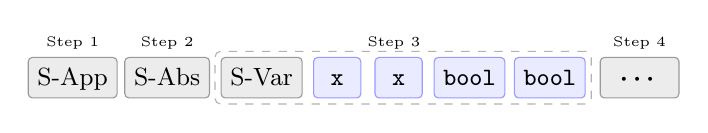
\begin{tikzpicture}[x=1.2cm, y=0.8cm]
    \tikzset{
        rule/.style={
            draw=gray!80, fill=gray!15,
            minimum height=5mm, minimum width=10mm,
            rounded corners=1.5pt, font=\small,
            text depth=0.25ex, text height=1.6ex
        },
        assign/.style={
            draw=blue!40, fill=blue!8,
            minimum height=5mm, minimum width=6mm,
            rounded corners=1.5pt, font=\small,
            text depth=0.25ex, text height=1.6ex
        },
    }

    % ==== Top row: steps ====
    \node[rule] at (0,0) {S-App};
    \node[rule] at (1,0) {S-Abs};
    \node[rule] (a0) at (2,0) {S-Var};

    % ==== Assignments row 
    \node[assign] (a1) at (2.80,0) {\tcode{x}};    
    \node[assign] (a2) at (3.45,0) {\tcode{x}};    
    \node[assign] (a3) at (4.20,0) {\tcode{bool}}; 
    \node[assign] (a4) at (5.05,0) {\tcode{bool}}; 

    \node[rule] at (6.0,0) {$\boldsymbol{\cdots}$};

    % ==== Step labels ====
    \node[above] at (0,0.3) {\tiny Step 1};
    \node[above] at (1,0.3) {\tiny Step 2};
    \node[above] at (3.4,0.3) {\tiny Step 3};
    \node[above] at (6.0,0.3) {\tiny Step 4};

    % ==== Bounding box around assignments ====
    \node[
        draw=gray!60,
        dashed,
        rounded corners=2pt,
        fit={(a0) (a4)},
        inner sep=2pt
    ] {};
\end{tikzpicture}

\setlength{\fboxsep}{1pt}
\caption{Synthesis decision sequence for $\app{(\abs{\tcode{x}}{\tcode{bool}}{\tcode{x}})}{\tcode{true}}$: 
\colorbox{gray!15}{\textsf{synthesis rules}} and 
\colorbox{blue!8}{\textsf{variable assignments}}.}
\label{fig:synthesis-sequence}
\end{figure}

As shown in \autoref{fig:synthesis-sequence}, the synthesis rules and variable assignments together form a synthesis decision sequence, which serves as a novel program representation in \mainname. 
Unlike traditional representations that treat programs as flat sequences of syntactic tokens (e.g., [$\lambda$, $x$, :, \tcode{bool}, $\dots$]), our representation is structured around the type correctness proof. Each token corresponds to a step in the proof construction process, directly capturing the hierarchical structure of type reasoning (as in \autoref{figure:sample-type-tree}). This enables the LM to learn the type system explicitly rather than attempting to reconstruct it from flat token sequences. Since this sequence represents a program synthesis process that determines both the resulting program and its type correctness proof, this representation embodies our \textbf{Derivation Vicinality} principle.

To support this proof-guided synthesis, we design a novel model architecture with dual-encoding: the encoder processes both the static natural language specification and the dynamically evolving synthesis goal at each step, providing rich typing context to the decoder. Details of this architecture are presented in \autoref{sec:implementation}.

\smallskip \noindent \textbf{Training.} Since our representation differs from traditional token sequences, the LM requires fine-tuning to generate synthesis decision sequences.
%
Our representation also offers \textbf{Data Usability}, as it is compatible with existing code generation datasets for the target language.
Given a corpus of programs, we construct their type correctness proofs via the type checker, convert the proofs into synthesis decision sequences using the correspondence between typing rules and synthesis rules, and obtain a training set in \mainname's representation. 


%DIF >  !TEX root=../manuscript.tex
\section{Translation from Typing Rules to Synthesis Rules \label{sec:meta}}

In this section, we introduce the necessary preliminaries on constrained Horn clauses and unification,    {\color{revblue}present } the user-provided specifications of the object language    {\color{revblue}(including terms and typing rules)} , and describe how typing rules are systematically translated into synthesis rules.

\subsection{Preliminaries}
\subsubsection{Constrained Horn Clauses}
\label{chc-intro}
Constrained Horn clauses (CHCs) are a fragment of first-order logic with applications to program verification and synthesis~\cite{DBLP:conf/synasc/GurfinkelB19}. A constrained Horn clause, in this setting, is a universally quantified implication of the canonical form:
\begin{center}
\begin{prooftree}[rule margin=0.5ex, separation=1em]
\hypo{P_1(\overline{x}_1)}
\hypo{P_2(\overline{x}_2)}
\hypo{\ldots}
\hypo{P_n(\overline{x}_n)}
\hypo{\phi(\overline{y})}
\infer5[(CHC)]{P(\overline{x}_0)}
\end{prooftree}
\captionof{figure}{General form of a constrained Horn clause.}
\label{T-Rule}
\end{center}
Each clause consists of zero or more premises, where each premise is a judgment formed by applying an uninterpreted predicate $P_i$ to terms $\overline{x}_i$. It also includes a constraint $\phi(\overline{y})$, a computable function over terms $\overline{y}$, and concludes with a single judgment $P(\overline{x}_0)$.
%
This rule states that the judgment $P(\overline{x}_0)$ can be derived whenever all the premises $P_i(\overline{x}_i)$ are derivable and the constraint $\phi(\overline{y})$ holds. Without loss of generality, we can assume that every variable of terms in $\overline{y}$ occurs among a term in the premises or conclusion, namely $FV(\overline{y})\subseteq \bigcup_{i=0}^n FV(\overline{x}_i)$, which ensures that the constraints are always deterministic and checkable given the premises and conclusion.

\begin{example}
Consider the typing rule \textsc{T-App} for function application in $\stlc$:
\begin{center}
\begin{prooftree}[rule margin=1ex, separation=1.5em]
\hypo{\stlctype{\Gamma}{p_1}{t_1 \rightarrow t_2}}
\hypo{\stlctype{\Gamma}{p_2}{t_1}}
\infer2[(T-App)]{\stlctype{\Gamma}{p_1~p_2}{t_2}}
\end{prooftree}
\end{center}
In CHC terminology: the predicates $P_1$ and $P_2$ are both the typing judgment predicate $\stlctype{\cdot}{\cdot}{\cdot}$; the terms $\overline{x}_1 = (\Gamma, p_1, t_1 \rightarrow t_2)$ and $\overline{x}_2 = (\Gamma, p_2, t_1)$ are the arguments to the premises; the conclusion $P(\overline{x}_0)$ is $\stlctype{\Gamma}{p_1~p_2}{t_2}$ with $\overline{x}_0 = (\Gamma, p_1~p_2, t_2)$; and the constraint $\phi$ is implicitly $\mathit{True}$.
\end{example}

It is well known that any Turing-computable function can be encoded using Horn clauses (HCs)~\cite{DBLP:journals/bit/Tarnlund77}. CHCs extend HCs by adding constraints $\phi(\overline{y})$, which allow expressing computable conditions (e.g., arithmetic comparisons, equality checks) directly within the clause. When all constraints are interpreted as $\mathit{True}$, CHCs collapse to ordinary HCs. Consequently, CHCs are at least as expressive as HCs, and any Turing-computable function can be expressed using CHCs, which ensures the expressiveness of our framework.

\subsubsection{Unification}
Unification is a fundamental operation in logic and computer science that finds substitutions to make two expressions structurally identical. Formally, given two terms $s$ and $t$, a \emph{unifier} is a substitution $\sigma$ such that $\sigma(s) = \sigma(t)$. When a unifier exists, the two terms are said to be \emph{unifiable}. Among all possible unifiers, the \emph{most general unifier} (MGU) provides the least restrictive solution: any other unifier can be obtained by further instantiating the MGU.

\begin{example}
Consider unifying an incomplete typing judgment $\stlctype{\tcode{empty}}{\sk{p_1}}{\arr{\sk{t_1}}{\sk{t_2}}}$ with another judgment $\stlctype{\sk{\Gamma_2}}{\left(\abs{\sk{x_1}}{\sk{t_3}}{\sk{p_3}}\right)}{\arr{\sk{t_3}}{\sk{t_4}}}$. The unification process matches corresponding positions: $\tcode{empty}$ with $\sk{\Gamma_2}$, $\sk{p_1}$ with $\abs{\sk{x_1}}{\sk{t_3}}{\sk{p_3}}$, and $\arr{\sk{t_1}}{\sk{t_2}}$ with $\arr{\sk{t_3}}{\sk{t_4}}$. This yields the MGU:
\[
\sigma = \{\sk{\Gamma_2} \mapsto \tcode{empty},\quad\sk{p_1} \mapsto \abs{\sk{x_1}}{\sk{t_3}}{\sk{p_3}},\quad\sk{t_1} \mapsto \sk{t_3},\quad\sk{t_2} \mapsto \sk{t_4}\}
\]
After applying $\sigma$, both terms become identical: $\stlctype{\tcode{empty}}{\left(\abs{\sk{x_1}}{\sk{t_3}}{\sk{p_3}}\right)}{\arr{\sk{t_3}}{\sk{t_4}}}$.

Note that unification is symmetric: it can bind variables from either term. Here, $\sk{\Gamma_2}$ is bound to a concrete value $\tcode{empty}$, while $\sk{t_1}$ and $\sk{t_2}$ are bound to other variables $\sk{t_3}$ and $\sk{t_4}$.
The MGU preserves maximum generality by not over-constraining variables. For instance, the substitution $\{\sk{\Gamma_2} \mapsto \tcode{empty}, \sk{p_1} \mapsto \abs{\sk{x_1}}{\sk{t_3}}{\sk{p_3}}, \sk{t_1} \mapsto \sk{t_3}, \sk{t_2} \mapsto \sk{t_4}, \sk{t_3} \mapsto \tcode{bool}\}$ is also a valid unifier, but it is not the MGU because it unnecessarily constrains $\sk{t_3}$ to $\tcode{bool}$.
\end{example}

In our synthesis framework, unification enables typing rules to be applied by aligning the schematic parameters in a rule's conclusion with the current synthesis goal. When a typing rule is selected, unification extracts the relationship between the goal's unknowns and the rule's parameters, propagating known information and establishing constraints between unknowns.
%
In this paper, we restrict ourselves to \emph{first-order unification}, where variables range only over terms and not over functions or predicates. 
First-order unification is decidable and admits efficient algorithmic solutions~\cite{DBLP:journals/jacm/Robinson65}, making it suitable for our synthesis framework.  {\color{revblue}This restriction excludes type systems that require }\emph{\color{revblue}higher-order unification}{\color{revblue}, which arises naturally with higher-order functions and polymorphism and is undecidable in general. Extending }\mainname {\color{revblue}to such systems would need a decidable fragment (e.g., patterns) or a different variable-acquisition mechanism, and our formal results do not automatically carry over.
} 

\subsection{Terms and Typing Rules}
\subsubsection{Terms}
\label{terms-intro}
We begin by defining the object language through a structured set of terms. A \emph{term} is a symbolic expression that represents programs, types, contexts, or other syntactic entities in the object language. Each term type is specified inductively: terms are constructed from constants, variables, and composite structures via constructors. For any given term type \tcode{T}, the syntax conforms to the general form:
\[\tcode{T} \,::=\, \tcode{c} \;\mid\; \tcode{v} \;\mid\; \tcode{k}(\tcode{T}_1, \ldots, \tcode{T}_n)\]
where \(\tcode{c}\) ranges over constants \(\mathcal{C}_\scode{T}\), \(\tcode{v}\) ranges over the global set of variables \(\mathcal{V}\), and \(\tcode{k}\) ranges over constructor symbols \(\mathcal{K}_\scode{T}\) of specified arity and parameter term types. 

The variable set $\mathcal{V}$ consists of symbolic names serving as placeholders to be instantiated by terms. In contrast, the sets of constants $\mathcal{C}_\scode{T}$ and constructors $\mathcal{K}_\scode{T}$ are determined by user-defined inductive type declarations. 
Built-in types such as \tcode{Int} and \tcode{String} are provided following conventional programming language syntax.

\begin{example}
Consider the following syntax for programs in $\stlc$:
\[
\tcode{Prog} ::= 
  \tcode{true} \;\mid\;
  \tcode{false} \;\mid\;
  \tcode{var}(\tcode{String}) \;\mid\;
  \tcode{app}(\tcode{Prog}, \tcode{Prog}) \;\mid\;
  \tcode{abs}(\tcode{String}, \tcode{Type}, \tcode{Prog})
\]
This yields the following instantiations of the general term pattern:
\begin{itemize}
  \item \textbf{Constants:} \(\mathcal{C}_{\tcode{Prog}} = \{\tcode{true}, \tcode{false}\}\)
  \item \textbf{Constructors:}
    \(\mathcal{K}_{\text{Prog}} = \{
      \tcode{var} : (\tcode{String}),\ 
      \tcode{app} : (\tcode{Prog}, \tcode{Prog}),\ 
      \tcode{abs} : (\tcode{String}, \tcode{Type}, \tcode{Prog})
    \}\)
\end{itemize}
Using this syntax, the program $\lambda x{:}\tcode{bool}.\, x$ is represented as the term $\tcode{abs}(\tcode{"x"}, \tcode{bool}, \tcode{var}(\tcode{"x"}))$. This term is constructed by applying the constructor $\tcode{abs}$ to three arguments: the string $\tcode{"x"}$, the type $\tcode{bool}$, and the subterm $\tcode{var}(\tcode{"x"})$.
\end{example}

\subsubsection{Categories of terms and substitutions} 
In general, terms may contain known and unknown components, so in the remainder of this paper, we do not explicitly annotate terms as in \autoref{sketch-label}. Below, we provide definitions for key concepts that will be used throughout the subsequent sections.
\begin{enumerate}
    \item \textbf{Ground terms} are terms constructed exclusively from constants and constructors, containing no variables. 
    They are fully specified expressions that require no further instantiation.

    \item A \textbf{substitution} is a mapping \(\sigma: \mathcal{V}_0 \to \mathcal{T}\), where \(\mathcal{V}_0\) is a subset of variables \(\mathcal{V}\), and \(\mathcal{T}\) is the set of all terms. A substitution replaces each variable \(v \in \mathcal{V}_0\) with a term \(\sigma(v) \in \mathcal{T}\).

    The \textbf{composition} of two substitutions $\sigma_i$ and $\sigma_j$, denoted $\sigma_i \sigma_j$, is defined such that for any variable $v \in \mathcal{V}$, $(\sigma_i \sigma_j)(v) = \sigma_i(\sigma_j(v))$. 
    This allows multiple substitutions to be applied sequentially.
    A substitution $\sigma$ can also operate on a list of terms $\overline{t} = [t_1, t_2, \ldots, t_n]$, yielding a new list $\sigma(\overline{t}) = [\sigma(t_1), \sigma(t_2), \ldots, \sigma(t_n)]$ where $\sigma$ is applied to each term individually.

    \item An \textbf{assignment} is a special case of a substitution whose codomain ranges over ground terms.
    %that is, it is a function $\sigma : \mathcal{V}_0 \to \mathcal{G}_\mathcal{T}$, where $\mathcal{G}_\mathcal{T} \subseteq \mathcal{T}$ is the set of ground terms. 
    Assignments serve as the ultimate objective of the synthesis, as we require that the typing judgments, as synthesis goals, can be instantiated with no remaining uncertainties.
\end{enumerate}


\subsubsection{Typing Rules and Type Derivation Trees}
We formalize the typing rules of the object language as CHCs for their expressiveness and standard structure, where each typing rule is provided by the user as a CHC shown in \autoref{T-Rule}.
%
The user should also provide at least one typing rule whose conclusion is $\welltyped{p}$, the top-level judgment asserting that program $p$ is well-typed. For example, in $\stlc$, this judgment can be defined as $\exists t.\; \stlctype{\tcode{empty}}{p}{t}$, meaning that the program $p$ is well-typed under the empty context.

A judgment $P(\overline{t})$, where $\overline{t}$ are ground terms, is \emph{derivable} from a given set of typing rules if there exists a finite derivation tree whose root is labeled with $P(\overline{t})$, each internal node corresponds to the application of a typing rule, and all constraints of typing rules are satisfied. The type derivation tree is precisely this tree structure that witnesses the derivability of a typing judgment.
%
From a logical perspective, a type derivation tree is a \textbf{type correctness proof}: it proves that the typing judgment at the root holds. This correspondence between derivation trees and proofs is central to our approach. Later, we will show that a synthesis derivation tree corresponds to constructing an \textbf{existential type correctness proof} when the program is unknown: the synthesis process simultaneously discovers the program and constructs a proof of its type correctness.

More formally, a \emph{type derivation tree} for a typing judgment $P(\overline{t})$ is defined as: (1) the root node is labeled with $P(\overline{t})$; (2) each node is labeled with a typing judgment $P_i(\overline{t_i})$, where all terms $\overline{t_i}$ are ground terms, and annotated with the typing rule    {\color{revblue}that } derives $P_i(\overline{t_i})$ under  {\color{revblue}a } certain instantiation; (3) the children of each internal node correspond to the premises of the applied typing rule; and (4) for each applied typing rule, all associated constraints are satisfied under the instantiation.

For example, \autoref{figure:sample-type-tree} shows a type derivation tree for the program $(\lambda x{:}\tcode{bool}.\, x)\; \tcode{true}$, which proves that this program has type $\tcode{bool}$ under the empty context. Consider the following subtree for the subterm $\lambda x{:}\tcode{bool}.\, x$:
\begin{center}
\begin{prooftree}[rule margin=1ex, separation=1em]
\hypo{\checkBinding{x{:}\tcode{bool}}{x}{\tcode{bool}}}
\infer1[(T-Var)]{\stlctype{x{:}\tcode{bool}}{x}{\tcode{bool}}}
\infer1[(T-Abs)]{\stlctype{\tcode{empty}}{\lambda x{:}\tcode{bool}.\, x}{\tcode{bool} \rightarrow \tcode{bool}}}
\end{prooftree}
\end{center}
In this subtree, the root node is labeled with the typing judgment $\stlctype{\tcode{empty}}{\lambda x{:}\tcode{bool}.\, x}{\tcode{bool} \rightarrow \tcode{bool}}$ and annotated with the typing rule \textsc{T-Abs}. Its child node is labeled with $\stlctype{x{:}\tcode{bool}}{x}{\tcode{bool}}$ and annotated with \textsc{T-Var}, which has a constraint $\checkBinding{x{:}\tcode{bool}}{x}{\tcode{bool}}$ that checks whether the variable $x$ with type $\tcode{bool}$ exists in the context.

The existence of a type derivation tree for $\welltyped{p}$ establishes that the program $p$ is well-typed. To enable this verification, there should be a type checker in the object language toolchain that constructs the type derivation tree for $\welltyped{p}$ given any well-typed program $p$.

\subsection{Synthesis rules}
\label{sec:meta-translation}

\subsubsection{Synthesis Judgments and Synthesis Goals}
As outlined in the overview, when some components of a typing judgment are unknown (e.g., the program to be synthesized), typing rules can be reformulated as synthesis rules to handle such uncertainties. 
A typing judgment $R(\overline{t})$ is converted into a \emph{synthesis judgment} $R(\overline{t}) \leadsto \theta$, where $R(\overline{t})$ denotes the \emph{synthesis goal}, and $\theta$ is the assignment synthesized for the goal. 
Semantically, $R(\overline{t}) \leadsto \theta$ is derivable iff, after applying $\theta$ to $\overline{t}$, all terms in $\theta(\overline{t})$ are ground and the typing judgment $R(\theta(\overline{t}))$ is derivable.

\subsubsection{Translation from Typing Rules into Synthesis Rules}
\begin{center}
\begin{prooftree}[rule margin=1ex, separation=1.5em]
\hypo{\unify{\overline{x}=\overline{x}_0}=\sigma}
\infer[no rule]1{\acquire{\sigma(\overline{x}_f)} = \sigma_0}
\hypo{P_1(\sigma_0\sigma(\overline{x}_1)) \leadsto \sigma_1}
\infer[no rule]1{P_2(\sigma_1\sigma_0\sigma(\overline{x}_2)) \leadsto \sigma_2}
\ellipsis{}{P_n(\sigma_{n-1}\ldots\sigma_0\sigma(\overline{x}_n))\leadsto \sigma_n}
\hypo{\ensure{\phi(\sigma_n\ldots\sigma_0\sigma(\overline{y}))}}
\infer3[(S-Rule)]{P(\overline{x}) \leadsto \sigma_n\ldots\sigma_0\sigma|_{\mvhzc(\overline{x})}}
\end{prooftree}
\captionof{figure}{Normal form of the synthesis rules}
\label{S-Rule}
\end{center}

A typing rule in \autoref{T-Rule} can be translated into a synthesis rule in \autoref{S-Rule} in the following manner:
\begin{enumerate}
  \item \textbf{Conclusion translation.} The conclusion $P(\overline{x}_0)$ of the typing rule is replaced by a synthesis judgment $P(\overline{x}) \leadsto \sigma_n \ldots \sigma_0 \sigma|_{\mvhzc(\overline{x})}$ (with the same predicate $P$), where $\overline{x}$ is a sequence of newly introduced variables and can be instantiated with respect to the synthesis goal. $\mvhzc(\overline{x})$ denotes the set of variables in $\overline{x}$, which are the only variables that need to be synthesized. 
  $\sigma_n \ldots \sigma_0 \sigma|_{\mvhzc(\overline{x})}$ indicates that the final assignment is restricted to only those variables in $\overline{x}$.

  \item \textbf{Adding unification.} The unification step is added at the beginning of the synthesis rule, which unifies the variables $\overline{x}$ in the synthesis goal with the variables $\overline{x}_0$ in the conclusion of the typing judgment, yielding a substitution $\sigma$ that is the MGU of the unification problem. 

  \item \textbf{Adding Free variables acquisition.} The variables appearing in $\overline{x}_0$ but not in any of the $\overline{x}_i$ are collected into $\overline{x}_f$, defined as $\overline{x}_f = \text{list}(\mvhzc(\overline{x}_0) \setminus \bigcup_{i=1}^n \mvhzc(\overline{x}_i))$. We refer to $\overline{x}_f$ as the \emph{free variables} of the synthesis rule: they may not be bound by any premise even after unification, and thus should be acquired from external sources, yielding the assignment $\sigma_0$.

  \item \textbf{Premises translation.} Each premise $P_i(\overline{x}_i)$ is replaced by $P_i(\sigma_{i-1} \cdots \sigma_0 \sigma(\overline{x}_i)) \leadsto \sigma_i$, where $\sigma_{i-1} \cdots \sigma_0 \sigma(\overline{x}_i)$ instantiates the original terms $\overline{x}_i$ with substitutions from previous steps, and $\sigma_i$ is the assignment synthesized for the subgoal $P_i(\sigma_{i-1} \cdots \sigma_0 \sigma(\overline{x}_i))$ ($i\geq1$).

  \item \textbf{Constraint translation.} The constraint $\phi(\overline{y})$ is translated into $\ensure{\phi(\sigma_n \ldots \sigma_0 \sigma(\overline{y}))}$, which checks whether it holds under the assignment $\sigma_n \ldots \sigma_0 \sigma$.    
\end{enumerate}


\begin{example}
For example, if we have the following typing rule:
\begin{center}
\begin{prooftree}[rule margin=1ex, separation=1em]
\hypo{P_1(x_1)}
\hypo{P_2(x_2, c(x_1,x_3))}
\hypo{\phi(x_0, x_3)}
\infer3[(T-Rule1)]{P(x_0, c(x_1,x_2))}       
\end{prooftree}
\end{center}
We can translate it into the following synthesis rule:
\begin{center}
\begin{prooftree}[rule margin=1ex, separation=0.7em]
\hypo{\unify{s_0=x_0,\, s_1=c(x_1, x_2)}=\sigma}
\infer[no rule]1{\acquire{\sigma(x_0)} = \sigma_0}
\hypo{P_1(\sigma_0\sigma(x_1)) \leadsto \sigma_1}
\infer[no rule]1{P_2(\sigma_1\sigma_0\sigma(x_2,\, c(x_1,x_3))) \leadsto \sigma_2}
\hypo{\ensure{\phi(\sigma_2\sigma_1\sigma_0\sigma(x_0, x_3))}}
\infer3[(S-Rule1)]{P(s_0, s_1) \leadsto \sigma_2\sigma_1\sigma_0\sigma|_{\mvhzc(s_0, s_1)}}
\end{prooftree}
\end{center}
\end{example}

\begin{lemma}
\label{rule-bijection}
There is a one-to-one correspondence between typing rules and synthesis rules.
\end{lemma}

\begin{proof}
The complete proof can be found in Appendix~\ref{sec:appendix-lemma1}.
\end{proof}


%DIF >  !TEX root=../manuscript.tex
\section{Synthesis System}
\label{sec:approach}
\autoref{fig:classfy-problem} presents the architecture of \mainname's system, which constructs synthesis derivation trees from which programs are extracted. The construction is achieved in \autoref{alg:synthtree} through a series of queries (\autoref{sec:synthtree-construction-query}), which can be resolved through two approaches corresponding to the dual requirements of our system: code generation (\autoref{sec:query-resolution-lm}) and training data preparation (\autoref{sec:translation}).

The central claim of this section is that constructing a synthesis derivation tree, which is the core of \mainname's framework, is equivalent to constructing an existential type correctness proof. A key insight underlying this equivalence is the isomorphism between type derivation trees and synthesis derivation trees (\autoref{sec:isomorphism}). 
This isomorphism ensures that the constructed synthesis derivation trees maintain the logical flow and dependencies inherent in the type-level reasoning, so that we can construct synthesis derivation trees to represent well-typed programs (\autoref{sec:soundness-completeness}).

\begin{figure}[t]
\centering

\includegraphics[width=0.75\textwidth]{assets/methods1.png}
\caption{Meta-system architecture of \mainname.}
\label{fig:classfy-problem}
\end{figure}

\subsection{Construction of Synthesis Derivation Trees}
In this subsection, we will first describe the application of synthesis rules (\autoref{sec:synthesis-rule-application}), then introduce the concept of synthesis derivation trees (\autoref{sec:synthesis-derivation-tree}), and finally present the algorithmic construction of synthesis derivation trees, where it is realized by a sequence of query resolutions (\autoref{sec:synthtree-construction-query}).
\subsubsection{Synthesis Rule Application}
\label{sec:synthesis-rule-application}
Each synthesis rule as in \autoref{S-Rule} specifies how to start from a partially instantiated typing judgment $P(\overline{x})$, search for an assignment $\sigma$ to all variables in $\overline{x}$, then derive $P(\sigma(\overline{x}))$ using the corresponding typing rule. This procedure can be detailed as follows:
\begin{enumerate}
    \item \textbf{Unification Step:} First unify the terms in the synthesis goal $P(\overline{x})$ with the terms in the conclusion of the typing rule, yielding the MGU $\sigma$. Once the unification is done, the other terms ($\overline{x}_i$, $\overline{x}_f$, and $\overline{y}$) should also be instantiated with $\sigma$ to match the synthesis goal.    {\color{revblue}If } the unification fails,   the synthesis goal is not derivable using this synthesis rule.

    % This step ensures that the synthesis goal is aligned with the conclusion of the original typing rule (under certain assignment $\theta$, the resulting $P(\meta{\theta(\skhzc{\overline{x}})})$ can be derived using the original typing rule), or the unification fails, in which case the synthesis goal is not derivable using this synthesis rule.

    \item \textbf{Acquisition Step:} Next acquire the assignment for all free variables $\overline{x}_f$ in the synthesis    {\color{revblue}rule (after being } instantiated by $\sigma$) from external sources. 
    \mainname can infer the term type of each variable to be synthesized based on the definitions of predicates and terms. The generated assignments must conform to the inductively defined syntax described in \autoref{terms-intro}; if any constant or constructor does not match the required term type, the acquisition step fails.

    % Free variables can be synthesized either before or after the synthesis of the subgoals. Suppose the synthesis is deferred until after the subgoals. In that case, it is possible to obtain assignments for some variables in $\sigma(\overline{x}_f)$ from among the various $\sigma_i$ (since $\sigma(\overline{x}_f)$ and $\sigma(\overline{x}_i)$ may have shared variables after the unification), postponing the obligation to assign these variables until the last possible moment.
    % However, in practice, it is rare for $\overline{x}_f$ and $\overline{x}_i$ to have no shared variables initially, but to share variables after being instantiated by $\sigma$. If such a situation arises, it is more likely due to the selection of an inappropriate synthesis rule.
    % Therefore, we adopt an eager design approach: synthesizing the assignment $\sigma_0$ for free variables immediately after the unification step. This design encourages the LM to generate the necessary assignment right after choosing the synthesis rule, ensuring semantic coherence throughout the synthesis process.

    \emergencystretch=2em \item \textbf{Sub-Derivation Steps:} Then, synthesize assignments for all subgoals in sequence. For each subgoal    {\color{revblue}$P_i(\sigma_{i-1}\ldots\sigma_0\sigma(\overline{x}_i)) \allowbreak\leadsto \sigma_i$} , begin with an instantiation for variables in $\overline{x}_i$ with the substitutions $\sigma_{i-1}, \ldots, \sigma_0, \sigma$ in previous steps.
    This refines the subgoal and propagates synthesis information from earlier subgoals. Subsequently, synthesize the assignment $\sigma_i$ for the current subgoal by recursively applying synthesis rules.

    \emergencystretch=0pt \item \textbf{Constraint Checking Step:} After all synthesis subgoals have been solved, \mainname checks whether the constraint $\phi(\overline{y})$  is satisfied under the combined assignment $\sigma_n \ldots \sigma_0 \sigma$. 
    % If the constraint is satisfied, the synthesis rule is considered successfully applied, and we proceed to the final step.

    \item \textbf{Assignment Collection Step:} In the final step, \mainname compose {\color{revblue}s}  all substitutions obtained during synthesis to form $\sigma_c = \sigma_n \ldots \sigma_0 \sigma$, and restrict {\color{revblue}s}  this assignment to only the variables occurring in $\overline{x}$, yielding the overall assignment $\theta = \sigma_c|_{\mvhzc(\overline{x})}$. 
\end{enumerate}

In steps (3) and (5), we assert without proof that the composed substitution $\sigma_c = \sigma_n \ldots \sigma_0 \sigma$ and the final collected $\theta$ are assignments. Specifically, $\sigma_c$ maps all variables in $\overline{x}$ and $\overline{y}$ to ground terms. This property can be formally established by induction on the structure of the synthesis derivation.

\begin{lemma}
\label{lemma:assignment}
For any successful application of the synthesis rule in \autoref{S-Rule}, the substitution $\sigma_c = \sigma_n \ldots \sigma_0 \sigma$ is an assignment, in the sense that $\forall i$, $\sigma_c(\skhzc{\overline{x}_i})$, $\sigma_c(\skhzc{\overline{x}})$, and $\sigma_c(\skhzc{\overline{y}})$ are all ground terms.
\end{lemma}
\begin{proof}
  %It is proved by induction on the structure of the synthesis derivation.
  The complete proof can be found in Appendix~\ref{sec:appendix-lemma2}.
\end{proof}
% With Lemma~\ref{lemma:assignment}, the successful application of a synthesis rule yields a valid assignment that can concretize the synthesis goal. We will see in the following that we can construct a synthesis derivation tree for the synthesis goal $\welltyped{\skhzc{p}}\leadsto\theta$, which is isomorphic to a type derivation tree of the target program $\theta(\skhzc{p})$.

\subsubsection{Synthesis Derivation Trees}
\label{sec:synthesis-derivation-tree}
To formalize the structure of synthesis derivations, we introduce the concept of synthesis derivation trees in analogy to type derivation trees in type systems. 

A \emph{synthesis derivation tree} is a rooted tree that witnesses the derivability of a synthesis judgment through the application of synthesis rules. More formally, a synthesis derivation tree for a synthesis judgment $P(\skhzc{\overline{t}}) \leadsto \theta$ is a tree where: (1) the root node is labeled with $P(\skhzc{\overline{t}}) \leadsto \theta$; (2) each node is labeled with a synthesis judgment and annotated with both the synthesis rule used and the assignment for its free variables; (3) the children of each internal node correspond to the subgoals of the annotated synthesis rule; (4) for each synthesis rule, all steps including unification, assignment acquisition, subgoals synthesis and constraint checking succeed.

By Lemma~\ref{lemma:assignment}, the existence of a synthesis derivation tree for a synthesis judgment $P(\overline{t}) \leadsto \theta$ guarantees that there is an assignment $\theta$ satisfying the synthesis goal $P(\overline{t})$, that is, $\theta$ maps all variables to ground terms and    {\color{revblue}$P(\theta(\overline{t}))$ } is derivable with respect to typing rules.

\subsubsection{Algorithmic Construction of Synthesis Derivation Trees}
\label{sec:synthtree-construction-query}
The algorithmic construction of synthesis derivation trees is the main focus of \mainname, whether through the interaction with LMs, or via the translation from type derivation trees.
For a synthesis goal of the form $P(\overline{t})$, the task is to synthesize an assignment $\theta$ and construct a synthesis derivation tree with the root node labeled $P(\overline{t}) \leadsto \theta$ by recursively applying synthesis rules as described in \autoref{sec:synthesis-rule-application}.

% The overall construction of the synthesis derivation tree follows a two-phase process:
% \begin{enumerate}
%     \item \textbf{Tree Expansion Phase:} Starting from the synthesis goal $P(\skhzc{\overline{t}})$, we select an appropriate synthesis rule $R$ to apply. We then sequentially perform unification, assignment acquisition (obtaining $\sigma_0$), and recursively synthesize subgoals to expand the synthesis derivation tree.
%     \item \textbf{Assignment Collection Phase:} After synthesizing assignments for all subgoals, we check whether the constraint is satisfied. If so, we can collect the assignment $\theta$ for the original synthesis goal and construct the synthesis derivation tree with a root node labeled $P(\skhzc{\overline{t}}) \leadsto \theta$, annotated with the synthesis rule $R$ and the assignment $\sigma_0$. 
%     If this synthesis goal has a sibling subgoal in another synthesis rule application, the resulting assignment $\theta$ can be used to instantiate the corresponding variables in that sibling subgoal, allowing the propagation of the synthesis information throughout the synthesis derivation tree.
% \end{enumerate}

\begin{algorithm}[tb]
  \caption{Synthesis Derivation Tree Construction}
  \label{alg:synthtree}
  \KwIn{A synthesis goal $P(\skhzc{\overline{t}})$}
  \KwOut{A synthesis derivation tree $T$ whose root node is labeled $P(\skhzc{\overline{t}}) \leadsto \theta$}
  \SetKwFunction{GenSynthTree}{GenSynthTree}
  \SetKwProg{Fn}{Function}{:}{}

   %DIFDELCMD < \Fn{\GenSynthTree{$P(\overline{t})$}}{
%DIFDELCMD <     Select a synthesis rule $R$ with conclusion $P(\overline{x}) \leadsto \ldots$
%DIFDELCMD <     \tcp*{Suppose $R$ is as \autoref{S-Rule}}
%DIFDELCMD <     

%DIFDELCMD <     Instantiate $\overline{x}$ with $\overline{t}$ in $R$\;
%DIFDELCMD <     $\sigma \gets$ MGU from the unification step of $R$\;
%DIFDELCMD <     \lIf{$\sigma = \bot$}{\Return{$\bot$}} 
%DIFDELCMD < 

%DIFDELCMD <     $\sigma_0 \gets \func{AcquireFreeVariableAssignment}(\sigma(\overline{x}_f))$\;
%DIFDELCMD <     \lIf{$\sigma_0 = \bot$}{\Return{$\bot$}}
%DIFDELCMD <     

%DIFDELCMD <     \ForEach{\textnormal{subgoal} $P_i(\sigma_{i-1} \ldots \sigma_1 \sigma(\overline{x}_i))$ \textnormal{of} $R$}
%DIFDELCMD <     {
%DIFDELCMD <         $T_i \gets \GenSynthTree{ $P_i(\sigma_{i-1} \ldots \sigma_1 \sigma(\overline{x}_i))$} $\;
%DIFDELCMD <         \lIf{$T_i = \bot$}{\Return{$\bot$}}
%DIFDELCMD <         $\sigma_i \gets$ assignment from the root node of $T_i$\;
%DIFDELCMD <     }
%DIFDELCMD <     

%DIFDELCMD <     \lIf{$\phi(\sigma_n \ldots \sigma_0 \sigma(\overline{y})) = \bot$}{\Return{$\bot$}}
%DIFDELCMD <     $\theta \gets \sigma_n \ldots \sigma_0 \sigma|_{\mvhzc(\overline{t})}$\;
%DIFDELCMD <     \Return{$\func{MakeTreeNode}(P(\overline{t}) \leadsto \theta, R, \sigma_0, T_1, \ldots, T_n)$}
%DIFDELCMD < }
%DIFDELCMD < %%%
  \Fn{\GenSynthTree{$P(\overline{t})$}}{
    Select a synthesis rule $R$ with conclusion $P(\overline{x}) \leadsto \ldots$
    \tcp*{Suppose $R$ is as \autoref{S-Rule}}

    Instantiate $\overline{x}$ with $\overline{t}$ in $R$\;
    $\sigma \gets$ MGU from the unification step of $R$\;
    \lIf{$\sigma = \bot$}{\Return{$\bot$}} 

    $\sigma_0 \gets \func{AcquireFreeVariableAssignment}(\sigma(\overline{x}_f))$\;
    \lIf{$\sigma_0 = \bot$}{\Return{$\bot$}}

    \ForEach{\textnormal{subgoal} $P_i(\sigma_{i-1} \ldots \sigma_0 \sigma(\overline{x}_i))$ \textnormal{of} $R$}
    {
        $T_i \gets \GenSynthTree{ $P_i(\sigma_{i-1} \ldots \sigma_0 \sigma(\overline{x}_i))$} $\;
        \lIf{$T_i = \bot$}{\Return{$\bot$}}
        $\sigma_i \gets$ assignment from the root node of $T_i$\;
    }

    \lIf{$\phi(\sigma_n \ldots \sigma_0 \sigma(\overline{y})) = \bot$}{\Return{$\bot$}}
    $\theta \gets \sigma_n \ldots \sigma_0 \sigma|_{\mvhzc(\overline{t})}$\;
    \Return{$\func{MakeTreeNode}(P(\overline{t}) \leadsto \theta, R, \sigma_0, T_1, \ldots, T_n)$}
}
 \end{algorithm}

This process is detailed in \autoref{alg:synthtree}. In this algorithm, only two functions act as black boxes: the selection of synthesis rules and the acquisition of assignments for free variables. Both can be viewed as query problems. Synthesis rule selection is a single-step query that chooses one rule from a finite set of candidates, while assignment acquisition is a multi-step query that constructs a ground term for each free variable using a finite set of constructors and constants.

Consequently, our approach reduces the synthesis problem to finding appropriate solvers for these two specific query problems. This makes our framework more general and modular, as the extracted query resolution problems can be implemented independently. 
Moreover, the in-time checking mechanisms (unification and constraint verification, etc.) in \autoref{alg:synthtree} significantly restrict the search space compared to naive enumeration-based approaches. 
%This structured decomposition not only simplifies implementation but also enables leveraging existing LMs tailored for query-based tasks to address each component effectively.

\subsection{Query Resolution}
\autoref{fig:classfy-problem} illustrates how query resolution serves as a central mechanism in constructing a synthesis derivation tree. Queries should be resolved to determine which synthesis rule to apply and how to instantiate variables. In the following, we present two complementary approaches for query resolution: employing LMs to make decisions during code generation (\autoref{sec:query-resolution-lm}), and translating type derivation trees to prepare supervised training data (\autoref{sec:translation}).

\subsubsection{Query Resolution using LMs}
\label{sec:query-resolution-lm}
In the code generation scenario, both query resolution functions are delegated to the LM, which, given the natural language input, acts as a decision-making component for synthesis rule selection and variable assignment.

\begin{itemize}
  \item \textbf{Selection of synthesis rules:} Given the natural language description, the current partially constructed synthesis derivation tree, and the synthesis goal, the LM is expected to choose a specific synthesis rule from the available rule set.

  \item \textbf{Assignment of free variables:} After a synthesis rule is selected and unification is performed, the LM is required to generate a sequence of constructors and constants, constructing ground terms for assigning free variables. 
  % These assignments fill in the concrete details (such as variable names, constants, or operators) that are not determined by the rule structure alone.
\end{itemize}

LM prediction is performed in a contextually aware manner, conditioned on multiple sources of information: (1) the natural language describing the desired program behavior; (2) the current synthesis derivation tree, which encodes both the ongoing synthesis process and the type derivation process via the isomorphism between type and synthesis derivation trees; and (3) the synthesis goal $P(\overline{t})$, which includes already synthesized program fragments and the current typing context.

The LM leverages its learned type-reasoning ability to generate the most appropriate synthesis rule and corresponding variable assignments by jointly reasoning about the semantic intentions conveyed by the natural language and the structural requirements encoded in the derivation tree. 
% More detailed information about how the LM receives the information and makes decisions can be found in Section~\ref{sec:implementation}. 

\subsubsection{Query Resolution through Type Derivation Tree Translation}
\label{sec:translation}
Beyond the code generation scenario in which natural language serves as input, \mainname requires curated training data to teach the LM how to interpret and solve synthesis queries. 
We generate such queries by translating existing type derivation trees of target programs, which involves recording the contextual information and the ground truth decision at each step of synthesis rule application.

% By capturing these query-answer pairs throughout the synthesis process, we can provide the LM with supervised training examples that demonstrate how to make appropriate synthesis rule selections and variable assignments at each decision point.
The translation is performed by traversing the type derivation tree. When we visit its root node, we begin constructing the synthesis derivation tree from the root node too. 
For the $i$-th child labeled $P_i(\overline{x}_i)$ of the current node $n_1$ in the type derivation tree, upon entering its corresponding subtree, we construct the synthesis derivation tree for the $i$-th subgoal $P_i(\sigma_{i-1} \ldots \sigma_0 \sigma(\overline{x}_i))$ too.

When we return to the node $n_1$, the synthesis derivation trees for all subgoals have been constructed, allowing us to build node $n_2$ in the synthesis derivation tree. At every stage of the synthesis process, there is a node in the type derivation tree corresponding to the current synthesis goal.

\begin{itemize}
  \item \textbf{Selection of synthesis rules:}  
  Assume the node $n_1$ is labeled with a typing judgment $P(\overline{x}_c)$, annotated with a typing rule $R$, and the synthesis goal is $P(\overline{x})$. Following the procedure in \autoref{sec:meta-translation}, we translate $R$ into a synthesis rule $R'$, which is the synthesis rule to be applied.

  \item \textbf{Assignment of free variables:}  
    Assume the typing rule $R$ has the form in \autoref{T-Rule}, and the synthesis rule $R'$ has the form in \autoref{S-Rule}. 
    Then $P(\overline{x}_c)$ is the concretization of both the conclusion $P(\overline{x}_0)$ of the typing rule and the synthesis goal $P(\overline{x})$ (   {\color{revblue}as will } be proved later). 
    Thus, $\overline{x}_0$ and $\overline{x}$ are unifiable, and the MGU $\sigma$ makes $\sigma(\overline{x}) = \sigma(\overline{x}_0)$ unifiable with $\overline{x}_c$. Therefore, there exists an assignment $\theta'$ such that $\theta'\sigma(\overline{x}_0) = \overline{x}_c$ and $\theta'$ covers $\mvhzc(\sigma(\overline{x}_0))$. Since $\mvhzc(\overline{x}_f) \subseteq \mvhzc(\overline{x}_0)$, we have $\mvhzc(\sigma(\overline{x}_f)) \subseteq \mvhzc(\sigma(\overline{x}_0))$, so $\theta'$ can also cover $\mvhzc(\sigma(\overline{x}_f))$. Let $\sigma_0 = \theta'|_{\mvhzc(\sigma(\overline{x}_f))}$ be the assignment for the free variables in the synthesis rule.
\end{itemize}

Since the translation begins from a valid type derivation tree, it is guaranteed to produce a valid synthesis derivation tree. In particular, the unification, assignment acquisition, and constraint checking steps will always succeed, and the synthesized assignment $\theta$ concretizes the original synthesis goal $P(\overline{x})$ to the typing judgment $P(\overline{x}_c)$ labeled at the root of the type derivation tree.

\begin{lemma}
\label{lemma:translation}
Let $T_1$ be a type derivation tree whose root node is labeled $P(\overline{x}_c)$, annotated with typing rule $R$, and $T_2$ be the translated synthesis derivation tree, whose root node is labeled $P(\overline{x}) \leadsto \theta$.
%where $\theta$ is synthesized by \autoref{alg:synthtree}.
If $\,\overline{x}$ is unifiable with $\overline{x}_c$, then in the application of the synthesis rule $R'$ that derives $P(\overline{x}) \leadsto \theta$, (1) the unification step, (2) the acquisition step, and (3) the constraint checking step will succeed, and (4) the synthesized assignment $\theta$ concretizes $P(\overline{x})$ to $P(\theta(\overline{x}))$, which is equal to $P(\overline{x}_c)$.
\end{lemma}
\begin{proof}
  %It is proved by induction on the structure of the type derivation tree $T_1$.
  The complete proof can be found in the Appendix~\ref{sec:appendix-lemma3}.
\end{proof}

With Lemma~\ref{lemma:translation}, we can conclude that given a type derivation tree $T_1$ whose root node is labeled $\welltyped{p_c}$, we can start from the synthesis goal $\welltyped{\sk{p}}$, where $\sk{p}$ is a variable representing the program to be synthesized, and construct a synthesis derivation tree $T_2$ by translating from $T_1$ such that the root node of $T_2$ is labeled $\welltyped{\sk{p}} \leadsto \theta$, where $\theta(\sk{p}) = p_c$.

\subsection{Isomorphism between Type Derivation Trees and Synthesis Derivation Trees}
\label{sec:isomorphism}
Since every synthesis rule is translated from a typing rule, and every synthesis subgoal in the synthesis rule corresponds to a premise in the typing rule, we can establish an isomorphism between synthesis derivation trees and type derivation trees.

\paragraph{Isomorphism of Derivation Trees}
A type derivation tree $T_1 = (V_1, r_1)$ (with node set $V_1$ and root $r_1$) and a synthesis derivation tree $T_2 = (V_2, r_2)$ are \emph{isomorphic} if there exists a bijection $\varphi: V_1 \to V_2$ satisfying the following conditions:
\begin{enumerate}
    \item Root Correspondence: $\varphi(r_1) = r_2$
    \item Child Order Preservation: For $v \in V_1$, if $\mathsf{children}_{T_1}(v) = [v_1, \ldots, v_k]$, where $\mathsf{children}_{T}(v)$ denotes the ordered list of $v$'s children in tree $T$, then $\mathsf{children}_{T_2}(\varphi(v)) = [\varphi(v_1), \ldots, \varphi(v_k)]$
    \item Label/Annotation Correspondence: For every $v \in V_1$ labeled with typing judgment $P(\overline{t}_c)$ and a typing rule, $\varphi(v)$ is labeled with synthesis judgment $P(\skhzc{\overline{t}}) \leadsto \theta$, annotated with the corresponding synthesis rule and assignment, where $\theta(\skhzc{\overline{t}}) = \overline{t}_c$
\end{enumerate}
We write $T_1 \cong T_2$ to denote that $T_1$ and $T_2$ are isomorphic, representing the same logical structure but in different forms.
%
The translation procedure described in \autoref{sec:translation} provides a systematic way to construct an isomorphic synthesis derivation tree from any given type derivation tree. During this process, for each node $n_1$ in the type derivation tree, we define the correspondence $\varphi(n_1) = n_2$, where $n_2$ is the node constructed by translating $n_1$. It is straightforward to verify that this bijection preserves the root nodes and the order of children, and, by Lemma~\ref{lemma:translation}, also preserves the correspondence of labels and annotations. Thus, $T_1 \cong T_2$, as captured by the following lemma.

\begin{lemma}
\label{lemma:isomorphism1}
For any type derivation tree $T_1$, there exists a synthesis derivation tree $T_2$, $T_1 \cong T_2$.
\end{lemma}

Conversely, we can construct a type derivation tree $T_1$ from a given synthesis derivation tree $T_2$, also preserving isomorphism. The construction is straightforward: we traverse $T_2$, and for each node labeled with the synthesis goal $P(\overline{t}) \leadsto \theta$, we create a corresponding node labeled with the typing judgment $P(\theta(\overline{t}))$ and annotate it with the appropriate typing rule. Similar to Lemma~\ref{lemma:translation}, we can inductively show that the resulting $T_1$ is a type derivation tree, and that the bijection between $T_1$ and $T_2$ ensures the isomorphism $T_1 \cong T_2$.

\begin{lemma}
\label{lemma:isomorphism2}
For any synthesis derivation tree $T_2$, there exists a type derivation tree $T_1$, $T_1 \cong T_2$.
\end{lemma}
\begin{proof}
  The complete proof can be found in the Appendix~\ref{sec:appendix-lemma4}.
\end{proof}

\subsection{Soundness and Completeness}
\label{sec:soundness-completeness}
We have established an isomorphism between type derivation trees (type correctness proofs) and synthesis derivation trees (existential type correctness proofs). 
%As a result, synthesis derivation trees both collect assignments to the variables in the synthesis goals and represent the type derivation process for the synthesized programs. 
Under the isomorphism, \mainname ensures that well-typed programs can always be \emph{extracted} from synthesis derivation trees, rather than relying on direct program synthesis without reference to their type correctness proofs.

% \paragraph{Extracting Well-Typed Programs}
The notions of ``extract'' and ``well-typed'' can be formally defined in the context of derivation trees. 
Given a synthesis derivation tree with root node labeled $\welltyped{\sk{p}} \leadsto \theta$, the extracted program is $\theta(\sk{p})$.    {\color{revblue}A } program $p_c$ is said to be well-typed if there exists a type derivation tree (type correctness proof) whose root node is labeled $\welltyped{p_c}$.

\begin{theorem}[Soundness]
Any program extracted from a synthesis derivation tree $T$ is well-typed.
\end{theorem}
\begin{proof}
Suppose the root node of $T$ is labeled $\welltyped{\sk{p}} \leadsto \theta$. By Lemma~\ref{lemma:isomorphism2}, there is a type derivation tree $T'$ such that $T \cong T'$. The root node of $T'$ is labeled $\welltyped{p_c}$, where $p_c = \theta(\sk{p})$ is the program extracted from $T$. By the definition of well-typed programs, $p_c$ is well-typed.
\end{proof}

\begin{theorem}[Completeness]
For any well-typed program $p_c$, there exists a synthesis derivation tree such that the program extracted from it is $p_c$.
\end{theorem}
\begin{proof}
There exists a type derivation tree $T_1$ whose root node is labeled $\welltyped{p_c}$. By Lemma~\ref{lemma:isomorphism1}, there exists a synthesis derivation tree $T_2$ such that $T_1 \cong T_2$. The root node of $T_2$ is labeled $\welltyped{\sk{p}} \leadsto \theta$, where $\theta(\sk{p}) = p_c$. Thus, the program extracted from $T_2$ is $p_c$.
\end{proof}

\begin{corollary}
The synthesis derivation tree $T$ guaranteed by the completeness theorem is precisely the tree obtained through the translation process described in \autoref{sec:translation}.
\end{corollary}

The soundness and completeness theorems ensure the correspondence between well-typed programs and synthesis derivation trees. This correspondence works in both directions: every well-typed program can be represented as a synthesis derivation tree (completeness), and every synthesis derivation tree yields a well-typed program (soundness). Together, these results confirm that constructing a synthesis derivation tree is equivalent to constructing an existential type correctness proof: the isomorphism with type derivation trees provides the proof structure, while the synthesized assignment provides the witness (the program) that makes the existential statement $\exists p.\; \welltyped{p}$ hold.
%DIF >  !TEX root=../manuscript.tex
\section{Language Model Design}
\label{sec:implementation}

\subsection{Model Architecture}
To better adapt to our proof-guided synthesis system and maximize token utilization efficiency, we design a novel encoder-decoder-based model architecture, illustrated in \autoref{fig:model-arch}.

Unlike standard encoder-decoder models that encode only a static input, our architecture features a \emph{dual-encoding} design that separately processes two distinct input streams: (1) the fixed natural language specification, and (2) the dynamically evolving synthesis goal at each step.

\paragraph{Static Encoding.} The natural language specification remains unchanged throughout the synthesis process. We encode it once at the beginning to produce a fixed sequence of hidden states that stays constant across all synthesis steps.

\paragraph{Dynamic Encoding.} The synthesis goal, which provides the \emph{dynamic typing context}, evolves at each step as the synthesis derivation tree grows. We re-encode the current synthesis goal at each step to capture the updated typing context. The encoder produces a separate sequence of hidden states for this dynamic input.

\paragraph{Cross-Attention Fusion.} The decoder accesses both encodings through cross-attention mechanisms. We concatenate the static encoding $H_s$ and dynamic encoding $H_d$ along the sequence dimension to form a unified key-value sequence $H = [H_s; H_d]$. The decoder's cross-attention layers then attend to this concatenated sequence, computing attention over both the task specification and the current typing context simultaneously. This design allows the model to jointly reason about both information sources when predicting the next synthesis decision.

\begin{figure}[t]
\centering

\includegraphics[width=0.9\textwidth]{assets/model_arc2.png}
\caption{Model Architecture for Constructing Synthesis Derivation Trees}
\label{fig:model-arch}
\end{figure}

As described in \autoref{sec:query-resolution-lm}, the query resolution task is delegated to the LM, which takes the natural language prompt, the synthesis decisions generated so far, and the current synthesis goal as input and outputs a token representing the synthesis rule or variable assignments.

Meanwhile, \mainname maintains a synthesis decision sequence where each newly generated token is appended, representing the next synthesis decision. This sequence incrementally constructs an existential type correctness proof. Due to its autoregressive nature, the growing sequence is fed to the transformer decoder, allowing the LM to leverage the full history of synthesis decisions when predicting the next token.

\paragraph{Model Inference Process.}
At each synthesis step:
\begin{enumerate}
    \item The current synthesis goal is extracted from the (incomplete) synthesis derivation tree.
    \item The encoder encodes the synthesis goal to provide \emph{dynamic typing context} to the LM.
    \item The decoder processes both encodings from the encoder, along with the previous synthesis decision sequence, generating the next token representing a synthesis decision.
    \item This new token is appended to the synthesis decision sequence and used to incrementally update the synthesis derivation tree as detailed in  \autoref{alg:synthtree}.
    \item The updated synthesis derivation tree yields either a new synthesis goal for the next iteration or, upon completion, a well-typed program together with its type correctness proof.
\end{enumerate}

\paragraph{Efficient Token Reuse through Incremental Construction.}
According to \autoref{alg:synthtree}, the synthesis derivation tree construction follows a serialized order, ensuring that each step only appends new decisions without modifying the existing sequence.
This property aligns naturally with the autoregressive generation paradigm of transformer decoders, where each new token is predicted based on all previously generated tokens.
%
As a result, we can reuse the transformer's key-value (KV) cache~\cite{DBLP:conf/mlsys/PopeDCDBHXAD23}: the intermediate attention states computed for earlier tokens in the decision sequence are cached and reused when generating subsequent tokens. This eliminates the need to recompute attention over the entire decision sequence at each decision-making step, significantly reducing the computational overhead from quadratic to linear in sequence length.

\paragraph{Model Configuration.}
Our dual-encoding architecture is built upon standard Transformer encoder-decoder models, where both the encoder and decoder follow the standard Transformer architecture~\cite{DBLP:conf/nips/VaswaniSPUJGKP17}. We evaluate on two pre-trained models: \textbf{CodeT5-220M}~\cite{DBLP:conf/emnlp/0034WJH21}, with  {\color{revblue}a } 12-layer encoder and  {\color{revblue}a } 12-layer decoder, 12 attention heads, a hidden dimension of 768, and approximately 220 million parameters; and \textbf{T5Gemma2-2B}~\cite{zhang2025t5gemma2seeingreading}, with  {\color{revblue}a } 26-layer encoder and  {\color{revblue}a } 26-layer decoder, 8 attention heads, a hidden dimension of 2304, and approximately 2 billion parameters. For both models, the static encoder and dynamic encoder share the same weights but process different input streams.

\subsection{Term Encoding}
\label{sec:term-encoding}
Terms, as defined in \autoref{terms-intro}, are inductively constructed from constants and constructors. Following the approach of GrammarT5~\cite{DBLP:conf/icse/ZhuL000C24}, we serialize the abstract syntax tree (AST) of a term using a pre-order traversal, outputting each constructor or constant as a token in sequence. When a term contains unknown variables (not yet instantiated during synthesis), we represent them using a unified unknown token $\langle?\rangle$.

For example, consider the STLC program $\tcode{abs}(\tcode{"x"}, \tcode{bool}, \tcode{var}(\tcode{"x"}))$, which represents the identity function $\lambda x{:}\tcode{bool}.\, x$. Its AST has the constructor $\tcode{abs}$ at the root, with three children: the constant $\tcode{"x"}$ (the variable name), the constant $\tcode{bool}$ (the type annotation), and the subtree $\tcode{var}(\tcode{"x"})$. The pre-order traversal yields the token sequence illustrated in \autoref{fig:term-encoding}.

\begin{figure}[tb]
\centering
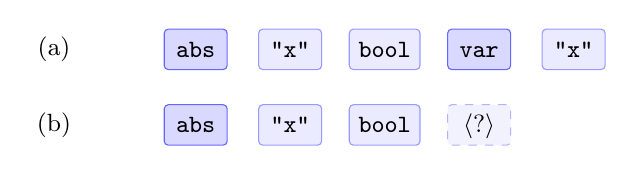
\begin{tikzpicture}[x=1.2cm, y=0.8cm]
    \tikzset{
        ctor/.style={
            draw=blue!60, fill=blue!15,
            minimum height=5mm, minimum width=8mm,
            rounded corners=1.5pt, font=\small,
            text depth=0.25ex, text height=1.6ex
        },
        const/.style={
            draw=blue!40, fill=blue!8,
            minimum height=5mm, minimum width=8mm,
            rounded corners=1.5pt, font=\small,
            text depth=0.25ex, text height=1.6ex
        },
        unknown/.style={
            draw=blue!30, fill=blue!5,
            minimum height=5mm, minimum width=8mm,
            rounded corners=1.5pt, font=\small,
            text depth=0.25ex, text height=1.6ex,
            dashed
        },
    }

    % ==== Full term encoding ====
    \node at (-1.5, 0) {\small (a)};
    \node[ctor] (c1) at (0,0) {\tcode{abs}};
    \node[const] (c2) at (1,0) {\tcode{"x"}};
    \node[const] (c3) at (2,0) {\tcode{bool}};
    \node[ctor] (c4) at (3,0) {\tcode{var}};
    \node[const] (c5) at (4,0) {\tcode{"x"}};

    % ==== Partial term encoding with unknown ====
    \node at (-1.5, -1.2) {\small (b)};
    \node[ctor] (p1) at (0,-1.2) {\tcode{abs}};
    \node[const] (p2) at (1,-1.2) {\tcode{"x"}};
    \node[const] (p3) at (2,-1.2) {\tcode{bool}};
    \node[unknown] (p4) at (3,-1.2) {$\langle?\rangle$};

\end{tikzpicture}

\setlength{\fboxsep}{1pt}
\caption{Term encoding as token sequences: 
\colorbox{blue!15}{\textsf{constructors}} and 
\colorbox{blue!8}{\textsf{constants}}.
(a) Full term $\tcode{abs}(\tcode{"x"}, \tcode{bool}, \tcode{var}(\tcode{"x"}))$.
(b) Partial term $\tcode{abs}(\tcode{"x"}, \tcode{bool}, \sk{e})$ with unknown variable.}
\label{fig:term-encoding}
\end{figure}

This encoding preserves the structural information of the term and can be uniquely decoded back to the original AST. The decoding is possible because each constructor has a fixed arity and known parameter types (as specified in the term definitions in \autoref{terms-intro}). When the decoder encounters a constructor token, it knows exactly how many subsequent tokens to consume and what types they should have, enabling unambiguous reconstruction of the tree structure. If the number of arguments or their types do not match the constructor's specification, the decoding fails and reports an error. During synthesis, the LM generates tokens following this same pre-order traversal order to construct terms for variable assignments. As each token is generated, the synthesis system incrementally decodes the sequence to reconstruct the corresponding AST, enabling immediate validation and integration into the synthesis derivation tree.

\subsection{Advanced Techniques for LM-Based Program Synthesis}
The program synthesis algorithm in \autoref{alg:synthtree} involves sequential actions at each node: selecting synthesis rules, acquiring variable assignments, and applying rules to update the synthesis derivation tree. 
%
To ensure the efficiency and correctness of this process, we implement pruning strategies that naturally correspond to the potential failures in synthesis rule application. 

At the syntactic level, we apply \emph{syntactic pruning}, which ensures the structural validity of synthesis derivation trees and enforces the well-formedness of generated sequences.
\emph{Syntactic pruning} is triggered instantly    {\color{revblue}after } a token is generated  {\color{revblue}in the following cases} : (1) the synthesis goal expects a synthesis rule to apply but the token stands for a term, or vice versa; (2) the predicate in the synthesis rule's conclusion differs from that of the synthesis goal; or (3) during term generation, the token corresponds to constructors or constants (see \autoref{terms-intro}) that mismatch the expected term type.
%
\begin{example}
Consider generating the term $\tcode{abs}(\tcode{"x"}, \tcode{bool}, \tcode{var}(\tcode{"x"}))$ using the term encoding from \autoref{sec:term-encoding}. Suppose the current token sequence is $[\tcode{abs}, \tcode{"x"}]$, meaning the LM has generated the constructor $\tcode{abs}$ and its first argument $\tcode{"x"}$ (the variable name). According to the constructor specification $\tcode{abs} : (\tcode{String}, \tcode{Type}, \tcode{Prog})$, the next token should be of type $\tcode{Type}$. If the LM generates $\tcode{var}$ (a $\tcode{Prog}$ constructor) instead of a valid type like $\tcode{bool}$, syntactic pruning immediately rejects this token because the expected type $\tcode{Type}$ does not match the actual type $\tcode{Prog}$.
\end{example}

At the type level, we apply \emph{type pruning}, which focuses on type-level correctness and relies on premise checking during the application of synthesis rules. 
If the unification step or constraint checking step fails, the corresponding search is immediately terminated. 
This prevents the exploration of synthesis paths that cannot lead to valid type correctness proofs.
%
\begin{example}
Consider applying the \rulename{T-Var} rule, which has a constraint $\checkBinding{\Gamma}{x}{t}$ that checks whether the variable $x$ with type $t$ exists in the context $\Gamma$. Suppose the current synthesis goal is $\stlctype{\Gamma}{\sk{e}}{\tcode{int}}$ where $\Gamma = \{f : \tcode{bool}, g : \tcode{int}\}$. If the LM selects $f$ to instantiate $\sk{e}$, the constraint checking step verifies $\checkBinding{\Gamma}{f}{\tcode{int}}$. Since $f$ has type $\tcode{bool}$ in $\Gamma$, not $\tcode{int}$, the constraint fails and type pruning terminates this branch. The correct choice would be $g$, which has the matching type $\tcode{int}$.
\end{example}

\emph{Syntactic pruning}, \emph{type pruning}, and the previously mentioned \emph{dynamic typing context} constitute a layered enhancement framework: 
\emph{syntactic pruning} serves as a prerequisite for \emph{type pruning}, since a structurally invalid synthesis derivation cannot be applied to perform type-level checking. 
Furthermore, without the successful application of synthesis rules, the intended synthesis goal cannot be extracted from the synthesis derivation tree. 
Should all three techniques be omitted, the model reduces to a standard encoder-decoder architecture that directly maps natural language inputs to sequences of synthesis decisions, lacking any mechanism to enforce structural or type-level correctness.

Beam search~\cite{DBLP:conf/aclnmt/FreitagA17} enables efficient exploration of multiple synthesis paths by maintaining the top-$k$ candidate sequences based on cumulative likelihood scores. At each step, rather than greedily selecting only the highest-probability token, beam search expands all $k$ beams and retains the top-$k$ sequences across all candidates.
When a branch is pruned due to syntactic or type errors, we terminate its sequence and discard its KV cache, while  {\color{revblue}the } remaining branches continue independently. This prevents invalid branches from wasting beam slots, ensuring all $k$ slots are reserved for branches that may lead to valid programs.
%DIF >  !TEX root=../manuscript.tex
\section{Evaluation \label{sec:evaluation}}
We design our evaluation to answer the following research questions.
\begin{itemize}
    \item \textbf{RQ1:} How does \mainname compare with    {\color{revblue}its base models across model scales and benchmarks} ?
    \item \textbf{RQ2:} How does each component of \mainname contribute   to the overall performance {\color{revblue}, and what runtime cost does it introduce} ?
    \item \textbf{RQ3:} How does   \mainname compare with  {\color{revblue}other reliability-oriented generation approaches, including } rejection sampling,    {\color{revblue}token-level constrained decoding, completion-engine repair, and iterative compiler-feedback repair} ?
    \item \textbf{RQ4:} How does \mainname compare with variants that generate the type derivation tree and the program separately instead of simultaneously?
\end{itemize}

\subsection{Experimental Setup}

\subsubsection{Benchmark}
To evaluate the generality of \mainname, our evaluation considers two languages with very different characteristics, SuFu~\cite{DBLP:journals/pacmpl/JiZPXH24} and Java.
%Correspondingly, we used two datasets: the SuFu dataset and the MBJP~\cite{DBLP:conf/iclr/AthiwaratkunGWL23} dataset.
\begin{itemize}
 \item \textbf{SuFu} is an ML-style functional language designed for automatic program optimization. This language uses a customized type system for extracting operations for optimization on data structures.
 %
 This language has limited code resources, making it representative for evaluating \mainname under low-resource conditions.

 We collect SuFu programs from its GitHub repository, which comprises 290 programs with test cases. For each program, we manually supply a natural language description, along with the relevant inductive definitions and library functions, thus collecting a dataset of code generation tasks.
 %
 This dataset is then split randomly into a training set of 80\% tasks and a test set of 20\% tasks.

 \item \textbf{Java} is a popular imperative language with a sophisticated type system. In a balance between the implementation cost and the expressiveness, we implement a subset of Java that preserves its core syntax while omitting advanced features like lambda expressions.

 We consider the MBJP dataset {\color{revblue}~\mbox{%DIFAUXCMD
\cite{DBLP:conf/iclr/AthiwaratkunGWL23} }\hskip0pt%DIFAUXCMD
} in our evaluation, which is the Java version of the popular MBPP dataset  . Our Java subset covers    {\color{revblue}the MBJP tasks admitted by our toolchain, which we split } randomly into a training set of    {\color{revblue}608 } tasks and a  {\color{revblue}held-out } test set of    {\color{revblue}67 tasks.
}

 \item \textbf{\color{revblue}HumanEval-Java} {\color{revblue}and }\textbf{\color{revblue}TransCoder-GFG} {\color{revblue}are two additional Java benchmarks that broaden the evaluation beyond MBJP. HumanEval-Java adapts the HumanEval problems to Java~\mbox{%DIFAUXCMD
\cite{DBLP:journals/corr/abs-2107-03374}}\hskip0pt%DIFAUXCMD
, and TransCoder-GFG collects the Java programs released with TransCoder~\mbox{%DIFAUXCMD
\cite{DBLP:conf/nips/LachauxROC20}}\hskip0pt%DIFAUXCMD
; both follow the task format of MBJP. 
HumanEval-Java uses a fixed split of 146 training and 16 test tasks, and TransCoder-GFG uses a fixed split of 414 training and 103 test tasks.
} \end{itemize}

More information about SuFu, Java, and the    {\color{revblue}dataset construction } can be found in Appendix~\ref{appendix-benchmark}.

\subsubsection{Models}
We implement \mainname based on CodeT5~\cite{DBLP:conf/emnlp/0034WJH21}, a family of encoder-decoder models for code understanding and generation. We adopt the 220M variant of CodeT5 as our base model for subsequent training and refer to our model as \mainname-220M. 
We also evaluate \mainname on T5Gemma2~\cite{zhang2025t5gemma2seeingreading}, a more recent encoder-decoder model family built upon Gemma 3. We adopt the 2B variant of T5Gemma2 as our base model and refer to this model as \mainname-2B. 

\subsubsection{Evaluation Metrics} 
\label{sec:evaluation-metrics}
To evaluate the quality of code generation, we adopt the metrics below, which respectively measure the correctness, effectiveness, and type correctness:

\begin{itemize}
    \item \textbf{Pass@k (k=1,10)~\cite{DBLP:journals/corr/abs-2107-03374}}: These metrics quantify the proportion of problems where at least one of the top-k generated candidates passes all reference test cases. Each generated candidate is executed against the test cases provided in the benchmark, and a candidate is considered correct only if it produces the expected output for all test cases. 
    %It's the standard and widely used method to quantify the correctness of generated code.

    \item \textbf{First Success Position (FSP)}: This metric is the mean rank of the first functionally correct candidate among the generated ones across the test set. It measures how early in the candidate list a correct solution appears, assessing the efficiency of output ranking {\color{revblue}; a problem with no correct candidate contributes the candidate-list length (10)} .

    \item \textbf{Compilation Error Rate (CER)}: This metric quantifies the proportion of generated candidates that fail to compile. 
    Since \mainname generates programs with type correctness guarantees, CER reflects the type system's effectiveness in catching compile-time errors. 
\end{itemize}

\subsubsection{Implementation Details}

We fine-tuned both \mainname-220M (based on CodeT5-220M) and \mainname-2B (based on T5Gemma2-2B) following a standard  {\color{revblue}supervised fine-tuning } procedure with the same set of hyperparameters to ensure a fair comparison. Each model was fine-tuned on the training set until convergence   {\color{revblue}.
} Since \mainname introduces a new representation that differs from standard code tokens    {\color{revblue}and thus faces a cold-start problem, we first } perform an initial    {\color{revblue}training } phase using a supervised fine-tuning dataset from OpenCoder~\cite{DBLP:journals/corr/abs-2411-04905} to    {\color{revblue}adapt the model } to this representation.
 {\color{revblue}At the same scale and on the same benchmark, each baseline--}\mainname{} {\color{revblue}pair is fine-tuned on the same training set. The exception is the two additional Java benchmarks, HumanEval-Java and TransCoder-GFG. There, }\mainname{\color{revblue}-2B builds on its MBJP fine-tuning, which avoids the cold-start problem, and is further trained on the training splits of the two benchmarks. The baselines, which generate ordinary code tokens and face no cold-start problem, are instead trained from the original T5Gemma2-2B, with the MBJP training tasks added to their own training sets for joint training.
} 

\subsection{Experimental Results}

\subsubsection{RQ1: Performance of \mainname}
\autoref{tab:model-results} summarizes the overall performance of \mainname {\color{revblue}, with models grouped by scale} .
%DIF < 
  For each    {\color{revblue}model scale and benchmark} , we compare the    {\color{revblue}fine-tuned baseline } (CodeT5-220M    {\color{revblue}or } T5Gemma2-2B) with  %DIFDELCMD < \mainname %%%
  {\color{revblue}our }\mainname{} {\color{revblue}model on the metrics above; the 2B group additionally covers the two Java benchmarks, HumanEval-Java and TransCoder-GFG} .

\begin{table}[ht]
\centering
\begin{threeparttable}
\caption{Comparison of Accuracy and Compilation Error Rate between    {\color{revblue}Base Models } and \mainname    {\color{revblue}at the 220M } and    {\color{revblue}2B Scales} }
\label{tab:model-results}
 %DIFDELCMD < \begin{tabular}{
%DIFDELCMD <     l 
%DIFDELCMD <     c
%DIFDELCMD <     c 
%DIFDELCMD <     c 
%DIFDELCMD <     c 
%DIFDELCMD <     c
%DIFDELCMD < }
%DIFDELCMD < %%%
  \begin{tabular}{
    l 
    l
    l
    c 
    c 
    c 
    c
}
 \toprule
   {\color{revblue}Scale } &  {\color{revblue}Benchmark }&  Model & {pass@1 (\%)\tnote{\updir}} & {pass@10 (\%)\tnote{\updir}} & {FSP\tnote{\downdir}} & {CER (\%)\tnote{\downdir}} \\
\midrule
 %DIFDELCMD < \multirow{4}{*}{SuFu} 
%DIFDELCMD <         %%%
  \multirow{4}{*}{220M}
         &  {\color{revblue}SuFu }&  CodeT5-220M         & 24.14 & 32.76 & 7.03 & 83.10 \\
        &        &    \mainname{\color{revblue}-220M      } &    \textbf{\color{revblue}37.93}  &    \textbf{\color{revblue}53.45}  &    \textbf{\color{revblue}5.03} & \textbf{\color{revblue}0.00}  \\
         %DIFDELCMD < \cmidrule{2-6}
%DIFDELCMD <         %%%
  \cmidrule(lr){2-7}
         &  {\color{revblue}MBJP }& {\color{revblue}CodeT5-220M         }& {\color{revblue}10.45 }& {\color{revblue}20.90 }& {\color{revblue}8.19 }& {\color{revblue}35.52 }\\
        &      &  \mainname-220M      &    \textbf{\color{revblue}11.94}  &    \textbf{\color{revblue}28.36}  &    \textbf{\color{revblue}7.94}  &    \textbf{\color{revblue}1.53}  \\
 \midrule
\multirow{8}{*}{2B}
         &  {\color{revblue}SuFu }& {\color{revblue}T5Gemma2-2B         }& {\color{revblue}25.86 }& {\color{revblue}37.93 }& {\color{revblue}6.66 }& {\color{revblue}71.21 }\\
        &      &  \mainname-2B        & \textbf{\color{revblue}36.21} & \textbf{\color{revblue}48.28} & \textbf{\color{revblue}5.53} & \textbf{0.00} \\
         %DIFDELCMD < \midrule
%DIFDELCMD < \multirow{4}{*}{Java} 
%DIFDELCMD <         %%%
  \cmidrule(lr){2-7}
         &    {\color{revblue}MBJP } &    {\color{revblue}T5Gemma2-2B         } &    {\color{revblue}13.43 } &    {\color{revblue}32.84 } &    {\color{revblue}7.46 }& {\color{revblue}29.55 } \\
        &       & \mainname{\color{revblue}-2B        }& \textbf{\color{revblue}25.37} & \textbf{\color{revblue}43.28} & \textbf{\color{revblue}6.36} & \textbf{\color{revblue}0.45} \\
        \cmidrule(lr){2-7}
        & {\color{revblue}HumanEval }&  T5Gemma2-2B &    {\color{revblue}31.25 } &    {\color{revblue}37.50 } &    {\color{revblue}6.50 } &    {\color{revblue}24.38 } \\
         %DIFDELCMD < \cmidrule{2-6}
%DIFDELCMD <         %%%
 &       &  \mainname   {\color{revblue}-2B        } &    \textbf{\color{revblue}50.00}  &    \textbf{\color{revblue}56.25}  &    \textbf{\color{revblue}4.75}  &    \textbf{\color{revblue}1.30}  \\
         \cmidrule(lr){2-7}
         &  {\color{revblue}GFG }& {\color{revblue}T5Gemma2-2B }& {\color{revblue}19.42 }& {\color{revblue}33.01 }& {\color{revblue}7.10 }& {\color{revblue}13.69 }\\
        &      &  \mainname-2B        & \textbf{\color{revblue}30.10} & \textbf{\color{revblue}46.60} & \textbf{\color{revblue}5.81} & \textbf{\color{revblue}2.75} \\
\bottomrule
\end{tabular}
\begin{tablenotes}
\footnotesize
\item \updir\, Higher is better; \downdir\, Lower is better;  \textbf{} %DIFAUXCMD
%DIFDELCMD < \item %%%
  {\color{revblue}metrics in } \autoref{sec:evaluation-metrics}  .
\end{tablenotes}
\end{threeparttable}
\end{table}

\mainname   improves code generation accuracy  %DIFDELCMD < \mainname%%%
  {\color{revblue}at both scales and on every benchmark: } pass@   {\color{revblue}1 rises from 24.14\% } to  %DIFDELCMD < \mainname%%%
  {\color{revblue}37.93\% (SuFu) and from 10.45\% to 11.94\% (MBJP) at 220M, and from 25.86\% } to  {\color{revblue}36.21\% (SuFu), 13.43\% to 25.37\% (MBJP), 31.25\% to } 50.00\%  %DIFDELCMD < \mainname%%%
  {\color{revblue}(HumanEval-Java), and 19.42\% to 30.10\% (TransCoder-GFG) at 2B; pass} @10    {\color{revblue}improves by 7.46--20.69 points on the same six benchmarks.
The largest gains are on SuFu } and  %DIFDELCMD < \mainname%%%
%DIFDELCMD < \mainname %%%
  {\color{revblue}HumanEval-Java, where the type constraints remove most uncompilable candidates while the base models often still produce them.
The 220M MBJP pass@1 gain is the smallest because there the type constraints mainly remove uncompilable candidates; the benefit shows up in pass@10 and CER instead, consistent with the failure analysis in Appendix~\ref{appendix-failure} (well-typed but wrong is the dominant residual mode).
}\mainname{} {\color{revblue}also drops CER to 0.00\% on SuFu and 0.45\% / 1.30\% / 2.75\% on the three Java benchmarks; the small residual Java CER comes from static-analysis errors the type system does not capture.
} 

 %DIFDELCMD < \mainname %%%
  {\color{revblue}To contextualize absolute performance, }\autoref{tab:decoder-only-compare} {\color{revblue}reports three larger decoder-only models (MiMo-7B} ,  {\color{revblue}Qwen3-14B, Qwen3-30B-A3B), prompted with the same task prompt in all conditions, alongside our two fine-tuned 2B encoder-decoder models.
Each prompted model produces one greedy candidate per task: the zero-shot condition uses only the task prompt, and the few-shot condition prepends three solved examples for the Java benchmarks and six examples for SuFu.
}

{\color{revblue}On SuFu the comparison favors }\mainname{}{\color{revblue}: none of the three solves a single task zero-shot, and few-shot prompting reaches at most 8 of 58, whereas } \mainname %DIFDELCMD < \mainname%%%
 -2B    {\color{revblue}solves 21; the low-resource language is where the type-guided representation delivers its advantage} .
On Java    {\color{revblue}the conclusion is the opposite: the prompted models solve 33--45 of 67 MBJP tasks, 3--14 of 16 HumanEval-Java tasks, and 38--52 of 103 TransCoder-GFG tasks, well above the fine-tuned 2B models. Moreover, few-shot prompting on Java brings little or no gain over zero-shot for these models, which suggests that they have seen this language extensively and may even have been trained on these benchmarks directly; we therefore flag a possible data-leakage risk for the Java comparison.
In any case, relative to its fine-tuned baseline T5Gemma2-2B, } \mainname %DIFDELCMD < \mainname%%%
 -2B    {\color{revblue}delivers a consistent improvement on all four benchmarks} .

   \begin{table}[ht]
\centering
\begin{threeparttable}
\caption{{\color{revblue}Pass@1 Comparison with Larger Decoder-Only Models}}
\label{tab:decoder-only-compare}
\begin{tabular}{l cc cc cc cc}
\toprule
& \multicolumn{2}{c}{{\color{revblue}MBJP (67)}} & \multicolumn{2}{c}{{\color{revblue}HumanEval-Java (16)}} & \multicolumn{2}{c}{{\color{revblue}TransCoder-GFG (103)}} & \multicolumn{2}{c}{{\color{revblue}SuFu (58)}} \\
\cmidrule(lr){2-3} \cmidrule(lr){4-5} \cmidrule(lr){6-7} \cmidrule(lr){8-9}
{\color{revblue}Model }& {\color{revblue}0-shot }& {\color{revblue}few-shot }& {\color{revblue}0-shot }& {\color{revblue}few-shot }& {\color{revblue}0-shot }& {\color{revblue}few-shot }& {\color{revblue}0-shot }& {\color{revblue}few-shot }\\
\midrule
{\color{revblue}MiMo-7B             }& {\color{revblue}34 }& {\color{revblue}33 }& {\color{revblue}3  }& {\color{revblue}10 }& {\color{revblue}38 }& {\color{revblue}43 }& {\color{revblue}0 }& {\color{revblue}6 }\\
{\color{revblue}Qwen3-14B           }& {\color{revblue}42 }& {\color{revblue}41 }& {\color{revblue}14 }& {\color{revblue}11 }& {\color{revblue}50 }& {\color{revblue}49 }& {\color{revblue}0 }& {\color{revblue}8 }\\
{\color{revblue}Qwen3-30B-A3B       }& {\color{revblue}42 }& {\color{revblue}45 }& {\color{revblue}13 }& {\color{revblue}14 }& {\color{revblue}52 }& {\color{revblue}52 }& {\color{revblue}0 }& {\color{revblue}6 }\\
\midrule
{\color{revblue}T5Gemma2-2B   }& \multicolumn{2}{c}{{\color{revblue}9}}  & \multicolumn{2}{c}{{\color{revblue}5}}  & \multicolumn{2}{c}{{\color{revblue}20}} & \multicolumn{2}{c}{{\color{revblue}15}} \\
 \mainname %DIFDELCMD < \mainname %%%
%DIFDELCMD < \mainname %%%
%DIFDELCMD < \mainname %%%
%DIFDELCMD < \mainname%%%
%DIFDELCMD < \mainname%%%
 -2B      & \multicolumn{2}{c}{{\color{revblue}17}} & \multicolumn{2}{c}{{\color{revblue}8}}  & \multicolumn{2}{c}{{\color{revblue}31}} & \multicolumn{2}{c}{{\color{revblue}21}} \\
\bottomrule
\end{tabular}
\begin{tablenotes}
\footnotesize
\item {\color{revblue}Cell entries are solved tasks at pass@1 for all models; the 0-shot condition uses the same prompt as the two fine-tuned models below.
}\end{tablenotes}
\end{threeparttable}
\end{table}
 

 %DIFDELCMD < \mainname %%%
%DIFDELCMD < 

%DIFDELCMD < %%%
 \subsubsection{RQ2: Contributions of Individual Components in \mainname}
   {\color{revblue}We } conduct an ablation study on the SuFu benchmark and the \mainname-220M model to quantify the contributions of each component in \mainname. Starting from the base case where \mainname synthesizes decision sequences with no checks, system components (syntactic pruning, type pruning, and dynamic typing context, as introduced in \autoref{sec:implementation}) are incrementally added, and the impact on performance metrics is evaluated at each stage. 
%DIF < \autoref{tab:ablation-combined} summarizes the results.
 \autoref{tab:ablation-combined} {\color{revblue}summarizes the results.
} 

\begin{table}[ht]
\centering
\setlength{\tabcolsep}{4pt}
\begin{threeparttable}
\caption{Sequential Ablation Study: Performance with Incremental Component Additions}
\label{tab:ablation-combined}
 %DIFDELCMD < \begin{tabular}{
%DIFDELCMD <     l 
%DIFDELCMD <     c@{\hspace{1em}}c
%DIFDELCMD <     c@{\hspace{1em}}c
%DIFDELCMD <     c@{\hspace{1em}}c
%DIFDELCMD <     c@{\hspace{1em}}c
%DIFDELCMD < }
%DIFDELCMD < %%%
  \begin{tabular}{
    l
    c@{\hspace{1em}}c
    c@{\hspace{1em}}c
    c@{\hspace{1em}}c
    c@{\hspace{1em}}c
    @{\hspace{0.5em}}c@{\hspace{0.5em}}c
}
 \toprule
\multicolumn{1}{l}{Components} &
\multicolumn{2}{c}{pass@1 (\%)\tnote{\updir}} &
\multicolumn{2}{c}{pass@10 (\%)\tnote{\updir}} &
\multicolumn{2}{c}{FSP\tnote{\downdir}} &
\multicolumn{2}{c}{CER (\%)\tnote{\downdir}}  &
\multicolumn{1}{c}{{\color{revblue}Time (s)}\tnote{\S}} &
\multicolumn{1}{c}{{\color{revblue}ms/step}\tnote{\S}}  \\
\cmidrule(lr){2-3} \cmidrule(lr){4-5} \cmidrule(lr){6-7} \cmidrule{8-9}  \cmidrule{10-11}
  & {   {\color{revblue}Score} } & {$\Delta$} & {   {\color{revblue}Score} } & {$\Delta$} & {   {\color{revblue}Score} } & {$\Delta$} & {   {\color{revblue}Score} } & {$\Delta$}  & {} & {}  \\
\midrule
Base (no checks)         & 24.14 & 0.00
                        & 36.21 & 0.00
                        & 6.78  & 0.00
                        & 74.26 & 0.00
                         & {\color{revblue}5.70 }& {\color{revblue}31.1 } \\
+ Syntactic Pruning         & 27.59 & +3.45
                        & 36.21 & 0.00
                        & 6.71  & -0.07
                        & 72.13 & -2.13
                         & {\color{revblue}5.34 }& {\color{revblue}32.4 } \\
+ Type Pruning            & \textbf{37.93} & \textbf{+13.79}
                        & 43.10 & +6.89
                        & 5.79  & -0.99
                        & \textbf{0.00} & \textbf{-74.26}
                         & {\color{revblue}11.07 }& {\color{revblue}43.7 } \\
+ Dynamic Typing Context       & \textbf{37.93} & \textbf{+13.79}
                        & \textbf{\color{revblue}53.45} & \textbf{+   {\color{revblue}17.24} }
                        & \textbf{\color{revblue}5.03}  & \textbf{\color{revblue}-1.75}
                        & \textbf{0.00}  & \textbf{-74.26}
                         & {\color{revblue}15.62 }& {\color{revblue}59.6 } \\
\bottomrule
\end{tabular}
\begin{tablenotes}
\footnotesize
\item[\,] \textit{\color{revblue}Score}: absolute value for each setting; $\Delta$: improvement relative to the base setting.
 \item[\S] \textit{\color{revblue}Time}{\color{revblue}: average per-task wall time; }\textit{\color{revblue}ms/step}{\color{revblue}: average wall time per decoding step.
} \end{tablenotes}
\end{threeparttable}
\end{table}

 %DIFDELCMD < 

%DIFDELCMD < %%%
  \paragraph{{\color{revblue}Functional contribution of each component.}}
{\color{revblue}The four metric columns of }\autoref{tab:ablation-combined} {\color{revblue}show which component contributes which improvement.
Syntactic pruning alone gives a moderate } pass@1    {\color{revblue}gain ($+3.45$); the turning point is type pruning, which lifts pass@1 by $+13.79$ and eliminates compilation errors outright (CER $74.26 \to 0.00$).
Dynamic typing context leaves } pass@1    {\color{revblue}and CER unchanged but improves } pass@10    {\color{revblue}($+17.24$ over the base) and FSP: it ranks correct candidates earlier rather than solving new tasks, which demonstrates the }\textbf{\color{revblue}Context Locality} {\color{revblue}property of~}\autoref{section:intro}{\color{revblue}.
}

\paragraph{{\color{revblue}How much the constraints prune.}}
{\color{revblue}To measure the pruning strength, we instrument the constrained decoder on the SuFu tasks (beam } 10  ,    {\color{revblue}330-step budget}\footnote{{\color{revblue}The longest decision sequence in the benchmark has 330 steps, so the budget suffices to derive every reference program.}}{\color{revblue}): syntactic pruning removes 59.1\% of all vocabulary proposals, and type pruning a further 8.2\%.
The lower rate is expected: type checking is more expensive, so it is applied only to the high-probability candidates about to enter the beam.
Such candidates are rarely ill-typed, yet pruning them matters, for they would otherwise expand within the beam and crowd out well-typed derivations.
Type checking during search is provisional (only completed AST fields are checked); the whole program is checked once when the derivation finishes, and this final check rejects 21.2\% of the completed candidates} .

%DIF < Overall, the sequential integration of grammar and type-aware constraints progressively enhances both correctness and robustness. 
   \paragraph{{\color{revblue}Whether the constraints over-prune.}}
{\color{revblue}By construction, pruning removes only ill-formed or ill-typed expansions, so every possibly correct derivation survives.
The residual risk is beam search itself, which retains only a fixed number of candidates per step: the correct candidate may in theory fall outside the beam, and the retained candidates then dead-end.
In our experiments this never occurs: under the beam-10 setting, no task dead-ends, and every task retains at least one grammar- and type-valid expansion at every step.
}


\paragraph{{\color{revblue}Runtime cost.}}
{\color{revblue}Each component increases the per-step cost ($31.1 \to 32.4 \to 43.7 \to 59.6$\,ms).
Syntactic pruning adds little (roughly $+4\%$); type pruning and the } dynamic typing context  \textbf{} %DIFAUXCMD
%DIFDELCMD < \autoref{section:intro}%%%
  {\color{revblue}cost considerably more, as the former invokes the type checker at every step and the latter additionally re-encodes the evolving synthesis goal.
The per-task totals move by $-6.38\%$ / $+94.00\%$ / $+173.88\%$ ($2.74\times$ base).
Syntactic pruning even lowers the per-task total: with little per-step overhead, it prunes ill-formed decisions early, so beams stay on well-formed derivations that finish sooner (164.6 versus 183.2 mean steps per task), and the $10\%$ fewer steps outweigh the per-step increase} .

\subsubsection{RQ3: Comparison with    {\color{revblue}Reliability-Oriented Generation Methods} }
 %DIFDELCMD < \mainname %%%
  {\color{revblue}We compare }\mainname{} {\color{revblue}with methods that pursue correct code by constraining or repairing the output of a trained model.
On MBJP, four such methods are applied on top of the same frozen T5Gemma2-2B checkpoint selected in RQ1, adding their own pruning or repair mechanisms on top: }\emph{\color{revblue}rejection sampling} ,    \emph{\color{revblue}SynCode}{\color{revblue}~\mbox{%DIFAUXCMD
\cite{ugare2024syncodellmgenerationgrammar}}\hskip0pt%DIFAUXCMD
, }\emph{\color{revblue}Repilot}{\color{revblue}(}\emph{\color{revblue}Copiloting the Copilots}{\color{revblue})~\mbox{%DIFAUXCMD
\cite{DBLP:conf/sigsoft/0003X023}}\hskip0pt%DIFAUXCMD
, and }\emph{\color{revblue}iterative compiler repair}{\color{revblue}.
All methods are evaluated on the same 67 tasks with 10 candidates each.
Because rejection sampling and repair need diverse draws rather than beam output, the ordinary control uses the temperature-sampling decoding protocol (temperature 0.8, top-$p$ 0.95), so its scores (14.93/23.88) differ from the beam-10 row of }\autoref{tab:model-results} {\color{revblue}(13.43/32.84); the }\mainname{\color{revblue}-2B row is identical in both tables.
}

{\color{revblue}Rejection sampling repeatedly draws candidates and keeps those that pass Java compilation, for up to ten ten-draw rounds (100 candidates) per task.
SynCode constrains decoding itself: at each step it masks the tokens that would violate a given grammar, so every output is syntactically well-formed. It is not originally implemented for Java, so we adapt it to the grammar of our Java subset.
Repilot pairs the LM with the Eclipse JDT completion engine: the partial program is maintained as a JDT document, and at each decoding position the engine is queried for the continuations it can legally complete, so that LM-proposed tokens inadmissible at that position are pruned.
Iterative compiler repair feeds }\texttt{\color{revblue}javac} {\color{revblue}diagnostics back to the model and regenerates the candidate for at most two rounds; the repair agent is the un-fine-tuned T5Gemma2-2B, since the fine-tuned model never learned to consume diagnostics.
}

 \begin{table}[ht]
\centering
\begin{threeparttable}
\caption{Comparison    {\color{revblue}of } \mainname  {\color{revblue}with Reliability-Oriented Generation Methods on Java} }
\label{tab:model-compare-sufu-java}
 %DIFDELCMD < \begin{tabular}{
%DIFDELCMD <     l
%DIFDELCMD <     l
%DIFDELCMD <     c
%DIFDELCMD <     c
%DIFDELCMD < }
%DIFDELCMD < %%%
  \begin{tabular}{
    l
    c
    c
    c
}
 \toprule
   {\color{revblue}Method } &  %DIFDELCMD < & %%%
 {pass@1 (\%)\tnote{\updir}} & {pass@10 (\%)\tnote{\updir}}  & {{\color{revblue}CER (\%)}\tnote{\downdir}}  \\
\midrule
 %DIFDELCMD < \multirow{3}{*}{SuFu} 
%DIFDELCMD <         %%%
  {\color{revblue}T5Gemma2-2B           } &    {\color{revblue}14.93 } &    {\color{revblue}23.88 } &    {\color{revblue}26.12 } \\
 %DIFDELCMD < & %%%
  {\color{revblue}\quad } + Rejection Sampling &    {\color{revblue}16.42 } &    {\color{revblue}28.36 }& {\color{revblue}0.00 } \\
 {\color{revblue}\quad + SynCode (adapt., compile-safe) } &  %DIFDELCMD < \mainname%%%
  {\color{revblue}14.93 } &  \textbf{} %DIFAUXCMD
  {\color{revblue}23.88 } &  \textbf{} %DIFAUXCMD
  {\color{revblue}21.34 } \\
 %DIFDELCMD < \midrule
%DIFDELCMD < \multirow{3}{*}{Java} 
%DIFDELCMD <         %%%
  {\color{revblue}\quad + Repilot/JDT       } &    {\color{revblue}14.93 } &    {\color{revblue}23.88 } &    {\color{revblue}25.97 } \\
 %DIFDELCMD < & %%%
  {\color{revblue}\quad } +    {\color{revblue}Iterative compiler repair } &    {\color{revblue}14.93 } &  %DIFDELCMD < \\
%DIFDELCMD <         %%%
  {\color{revblue}23.88 } &  {\color{revblue}17.31 }\\
 \mainname   {\color{revblue}-2B          } & \textbf{\color{revblue}25.37} & \textbf{\color{revblue}43.28}  & \textbf{\color{revblue}0.45}  \\
\bottomrule
\end{tabular}
 \begin{tablenotes}
\footnotesize
\item {\color{revblue}\updir\,/\downdir\, Higher/lower is better.
}\end{tablenotes}
 \end{threeparttable}
\end{table}

%DIF <  \autoref{tab:model-compare-sufu-java} compares the pass@1 and pass@10 results of three model variants (CodeT5-220M, CodeT5-220M with rejection sampling, and \mainname-220M) on both the SuFu and Java benchmarks.
   {\color{revblue}None of the four external baselines significantly improves functional correctness over the ordinary control:
rejection sampling adds three solved tasks at pass@10 (19 vs.\ 16 of 67) and one at pass@1 (11 vs.\ 10; McNemar $p=1.00$ and $p=0.25$);
SynCode, Repilot, and iterative repair leave the solved sets exactly unchanged (10/67 and 16/67);
Repilot's pruning rarely fires: following the original Repilot implementation, punctuation and keyword tokens are accepted without querying the engine, and the completion list at an incomplete position is permissive, so compilation errors barely move (26.12\% $\to$ 25.97\%);
iterative repair repairs 59 candidates' compilability (compile errors 175$\to$116 of 670) yet leaves the solved sets unchanged.
} \mainname %DIFDELCMD < 

%DIFDELCMD < %%%
%DIFDELCMD < \mainname %%%
  {\color{revblue}-2B solves 17/67 at } pass@1 and  {\color{revblue}29/67 at } pass@10  %DIFDELCMD < \mainname %%%
  {\color{revblue}with 3 of 670 candidates failing to compile, the best of all compared methods.
External reliability mechanisms (} post-hoc    {\color{revblue}filtering, token-level grammar masking, completion-engine repair, compiler-feedback regeneration) never change the model's own preference and distribution over output tokens, whereas }\mainname{} {\color{revblue}explicitly encodes the typing rules into the model and helps it better learn the program distribution} , demonstrating the    {\color{revblue}importance of the } \textbf{Type Explicitness}    {\color{revblue}property in~} \autoref{section:intro}.

\subsubsection{RQ4: Comparison with Separated Type-Code Generation}
   {\color{revblue}We } compare \mainname with approaches that separate type reasoning and code generation.
   {\color{revblue}Both variants fine-tune } CodeT5-220M    {\color{revblue}to emit a single sequence that concatenates the two parts, differing only in their order: }\emph{\color{revblue}Type-First} {\color{revblue}generates the sequence } of typing rules (forming the type derivation tree)    {\color{revblue}first and then the code on its basis, whereas }\emph{\color{revblue}Code-First} {\color{revblue}generates the code first and then the } typing rules as its type  %DIFDELCMD < \mainname%%%
  {\color{revblue}reasoning.
All settings are evaluated on the same SuFu and MBJP test sets with 10 candidates each} .

\begin{table}[ht]
\centering
\begin{threeparttable}
\caption{Comparison: Separated vs. Integrated Type-Code Generation}
\label{tab:sequential-compare}
\begin{tabular}{
    l
    l
    c
    c
    c
    c
    c
}
\toprule
Language & Model & {pass@1 (\%)\tnote{\updir}} & {pass@10 (\%)\tnote{\updir}} & {CER (\%)\tnote{\downdir}} & {FSP\tnote{\downdir}} & {Avg Tokens\tnote{\downdir}} \\
\midrule
 %DIFDELCMD < \multirow{3}{*}{SuFu}
%DIFDELCMD <         %%%
  \multirow{4}{*}{SuFu}
         &    {\color{revblue}CodeT5-220M                }& {\color{revblue}24.14 }& {\color{revblue}32.76 }& {\color{revblue}83.10 }& {\color{revblue}7.03 }& \textbf{\color{revblue}405} \\
        & {\color{revblue}CodeT5-220M } + Type-First   & 31.03 & 36.21 & 64.31 & 6.57 & 752 \\
        &    {\color{revblue}CodeT5-220M } + Code-First   & 29.31 & 39.66 & 56.72 & 6.28 & 752 \\
        & \mainname-220M             & \textbf{37.93} & \textbf{\color{revblue}53.45} & \textbf{0.00} & \textbf{\color{revblue}5.03} &  \textbf{} %DIFAUXCMD
  {\color{revblue}410 } \\
\midrule
 %DIFDELCMD < \multirow{3}{*}{Java}
%DIFDELCMD <         %%%
  \multirow{4}{*}{Java}
         &    {\color{revblue}CodeT5-220M                }& {\color{revblue}10.45 }& {\color{revblue}20.90 }& {\color{revblue}35.52 }& {\color{revblue}8.19 }& {\color{revblue}142 }\\
        & {\color{revblue}CodeT5-220M } + Type-First   & \textbf{11.94} & 26.87 & 37.61 & \textbf{7.36} & 247 \\
        &    {\color{revblue}CodeT5-220M } + Code-First   & 8.96 & 22.39 & 31.49 & 8.21 & 247 \\
        & \mainname-220M             & \textbf{11.94} & \textbf{28.36} & \textbf{\color{revblue}1.53} & 7.94 & \textbf{129} \\
\bottomrule
\end{tabular}
 \begin{tablenotes}
\footnotesize
\item {\color{revblue}\updir\,/\downdir\, Higher/lower is better.
}\item \emph{\color{revblue}Avg Tokens}{\color{revblue}: length of the generated sequence in each model's own vocabulary, excluding comments.
}\end{tablenotes}
 \end{threeparttable}
\end{table}

 %DIFDELCMD < \autoref{tab:sequential-compare} %%%
%DIFDELCMD < \mainname %%%
  {\color{revblue}Adding separated type reasoning improves over the ordinary trained baseline on both languages (e.g., Type-First 31.03 vs.\ 24.14 } pass@ {\color{revblue}1 on SuFu), and unifying the two into one process improves further: both separated variants trail }\mainname{} {\color{revblue}on pass} 10  %DIFDELCMD < \mainname %%%
 and    {\color{revblue}CER (on Java pass@1, Type-First merely ties }\mainname{}{\color{revblue}).
Because neither variant constrains decoding, their CER remains high (56.72--64.31 on SuFu} ), whereas  %DIFDELCMD < \mainname %%%
%DIFDELCMD < 

%DIFDELCMD < %%%
%DIFDELCMD < \mainname %%%
%DIFDELCMD < \mainname %%%
  \mainname{} {\color{revblue}outputs only type-valid programs.
In terms of token length, fully unifying type reasoning and code is far more economical than outputting them separately: the unified decision sequence (410 on SuFu, } 129    {\color{revblue}on Java) saves 342 and 118 tokens respectively against appending the typing rules to plain code tokens (752 and } 247 %DIFDELCMD < 

%DIFDELCMD < %%%
%DIFDELCMD < \mainname%%%
  {\color{revblue}).
It is even comparable to, or slightly shorter than, the plain code tokens alone (405 on SuFu, 142 on Java): a type derivation rule absorbs the redundant syntactic elements of the code (such as equals signs and semicolons) into a single rule token, so our representation adds little and sometimes removes tokens.
These results support the } \textbf{Derivation Vicinality}    {\color{revblue}paradigm of } \mainname   {\color{revblue}, that interleaving each program fragment with its type derivation is more accurate and more efficient than generating them separately.
} 

 \subsection{{\color{revblue}Limitations and Future Work}} \label{sec:limitations}
\paragraph{{\color{revblue}Dependence on the encoder-decoder architecture.}}
{\color{revblue}The current architecture is designed for encoder-decoder models: at each synthesis step, an encoder processes the evolving synthesis goal to provide the dynamic typing context.
The representation itself carries over to a decoder-only model unchanged; what changes is the architecture, and with it the cost of the dynamic typing context.
In a decoder-only model, supplying the context would mean prefilling the current typing context after the derivation prefix at every step and removing it again before the next step, so its key-value entries are recomputed at every step and never reused by later steps, and the computation is awkward to schedule.
We leave this adaptation to future work.
}

\paragraph{{\color{revblue}Dynamically typed languages.}}
{\color{revblue}The current design of }\mainname {\color{revblue}relies on a type system in which the type derivation of a program can be computed automatically from the program text, so that existing code can be converted into our decision-sequence format.
Dynamically typed languages such as Python still have typing rules to a degree, but the type derivation cannot be read off the program text alone, since types depend on control flow and runtime information.
As a result, decision sequences cannot be automatically extracted from existing programs, which breaks the }\textbf{\color{revblue}Data Usability} {\color{revblue}property of~}\autoref{section:intro} {\color{revblue}and with it the training-data pipeline.
Parsing and adapting such languages is left to future work.
}

\paragraph{{\color{revblue}Type-system expressiveness.}}
{\color{revblue}Both evaluated type systems are relatively simple compared with the mainstream languages that have evolved over decades, such as C++: the implemented Java subset omits subtyping hierarchies, overload resolution, and mutable-state-related features, and SuFu's type system targets fusion optimization.
The framework itself is not confined to such systems: typing rules are formulated as constrained Horn clauses (Sec.~\ref{sec:meta}), which can in principle describe more complex type systems and their languages.
The restriction is practical rather than conceptual: writing and modeling the concrete typing rules and designing the parser for a richer system make experimentation much harder, and our measurements on SuFu and the Java subset do not establish how the approach scales to such languages.
Migrating }\mainname{} {\color{revblue}to richer type systems, and even to systems such as linear types that can to some extent guarantee functional properties of the code, is a direction for future work.
}

%DIF >  !TEX root=../manuscript.tex

 \section{Related Work}\label{sec:related}

\subsection{Rejecting Invalid Generations}
%Our approach enforces a symbolic constraint expressed in CHCs. 
Existing studies have primarily explored \emph{external} enforcement of symbolic constraints    {\color{revblue}on } LMs.
%
A common baseline is the \emph{generate-and-validate} approach~\cite{DBLP:conf/sigsoft/ZhuSXZY0Z21,DBLP:conf/popl/LongR16}, which repeatedly generates code and checks it with an external validator (e.g., a compiler) until a valid candidate is found. While this ensures constraint satisfaction, it is often inefficient due to a high rate of invalid generations.

To address this, \emph{constrained decoding} techniques perform on-the-fly validation during token generation, discarding tokens that cannot lead to a valid complete program. This proactive strategy improves efficiency and has been applied to enforce various constraints, including syntactic correctness~\cite{ugare2024syncodellmgenerationgrammar}, type correctness~\cite{DBLP:journals/corr/abs-2504-09246}, and vulnerability avoidance~\cite{DBLP:conf/issre/StorhaugLH23}. However, such token-level pruning can also distort the LM's output distribution~\cite{DBLP:conf/nips/ParkWBPD24}. We compare with rejection sampling {\color{revblue}, grammar-constrained decoding (SynCode), completion-engine repair (Repilot), and iterative compiler-feedback repair } in our evaluation (\autoref{tab:model-compare-sufu-java})  .

Critically, both strategies enforce constraints \emph{externally}. As discussed, externally enforced constraints do not modify the LM's internal reasoning process. Consequently, the model's internal distribution may become skewed, potentially assigning low probability to correct code snippets due to inaccurate assessments of their typability.

\subsection{Internalizing Symbolic Constraints}
% * Grammar derivation tree
% * tare
% * AutoRefine
Another line of research aims to expose the reasoning process of symbolic constraints to the LMs, thereby guiding them to learn to satisfy the constraints.
%
By externalizing the complexity of constraint reasoning, this paradigm relieves LMs from implicitly inferring intricate symbolic rules from plain text. Offloading constraint learning to the representation allows LMs to allocate more capacity to other critical aspects, such as program semantics and algorithmic logic. This reallocation of modeling resources leads to improved generation quality that scales effectively with model size, mirroring the benefits observed in syntactic representations for grammatical learning~\cite{DBLP:conf/acl/LiangZ0LLXCZZZC25}.

Grammar-based encoding~\cite{DBLP:conf/acl/YinN17,DBLP:conf/aaai/SunZXSMZ20,DBLP:conf/icse/ZhuL000C24} represents one such approach, where programs are parsed into ASTs and serialized into sequences of grammar rules for training and inference. 
%DIF < This explicit syntactic representation helps models learn grammatical constraints more effectively. 
Grammar-based encoding can be viewed as a special case of our framework when grammar rules are expressed as CHCs. Our    {\color{revblue}implementation and evaluation exercise this generality on type-correctness constraints in two languages; other CHC-representable constraint families remain a formal possibility that we do not evaluate} .

Tare~\cite{DBLP:conf/icse/ZhuSZXZ23} introduces a neural approach for learning Java's type system in program repair, using specialized components to encode typing contexts and subtyping relations. While it predicts both code and types, Tare is specifically tailored to a subset of Java's type system and operates through AST traversal without achieving full type explicitness, which is a key distinction from our work.

Refine4LLM~\cite{DBLP:journals/pacmpl/CaiHSLLSD25} generates programs through sequential refinement rule applications, transforming specifications into concrete programs while ensuring syntactic and functional correctness. However, it requires training data containing refinement processes, which are scarce in practice, and is specific to a particular refinement calculus. In contrast, our approach utilizes readily available programs for training given a type checker, and    {\color{revblue}the CHC formulation extends in principle to constraints beyond type correctness} .

\subsection{Type-Guided Program Synthesis}
Our approach is inspired by type-guided program synthesis~\cite{DBLP:journals/pacmpl/GuoJJZWJP20, DBLP:conf/pldi/GuriaFH21, DBLP:conf/pldi/PolikarpovaKS16, DBLP:conf/pldi/OseraZ15}, which employs synthesis rules to produce type-correct programs. These approaches also guarantee type correctness by construction; however, they are designed for classical enumerative or constraint-based synthesis algorithms, not for neural code generation.

In contrast, our work addresses three challenges that arise when adapting type-guided synthesis to LMs.
First, existing synthesis systems do not provide a code representation suitable for LM training. We design synthesis decision sequences that can be derived from existing programs via type derivation trees, enabling the use of readily available codebases as training data.
Second, existing systems do not enforce the structural correspondence between type derivations and synthesis derivations. We design our synthesis rules to satisfy Type Explicitness and Derivation Vicinality, establishing an isomorphism that makes type reasoning fully explicit in the generated sequences.
Third, existing systems do not consider neural architectures for learning type systems. We propose a dual-encoding architecture that enables LMs to effectively learn and utilize type constraints during generation.
%DIF >  !TEX root=../manuscript.tex

\section{Conclusion \label{sec:conclusion}}
This paper presents \mainname, a proof-guided approach that guarantees type correctness in code generation by constructing existential type correctness proofs through a synthesis process. Through a synthesis system isomorphic to the type system and a synthesis decision sequence representation, \mainname ensures that constructing a synthesis derivation tree is equivalent to constructing an existential type correctness proof, thereby eliminating type errors during code generation, while significantly improving overall generation performance. 

Beyond type correctness, \mainname's    {\color{revblue}CHC foundation suggests a route toward richer constraint families, such as } safety verification and the generation of other structural data {\color{revblue}; instantiating and evaluating these extensions remains future work} . Our core insight---that aligning program representations with underlying proof systems enhances   generation performance---opens promising directions    {\color{revblue}in } other domains where structural constraints matter.

% \section*{Data-Availability Statement}
% An anonymized artifact supporting this paper—including experimental results, datasets, and source code—is available in an anonymous repository at \url{https://anonymous.4open.science/r/tacs-EF32}. We plan to submit this artifact for Artifact Evaluation upon paper notification.

\bibliographystyle{ACM-Reference-Format}
\bibliography{bibtex}

\newpage
\appendix
%DIF >  !TEX root=../manuscript.tex
\section{Proofs for Some Lemmas Used in the Paper}

\subsection{Proof for Lemma~\ref{rule-bijection}}
\label{sec:appendix-lemma1}
\begin{lemma}
There is a bijection $\varphi$ between typing rules and synthesis rules.
\end{lemma}
\begin{proof}

$\varphi$ can be proven to be a bijection by showing that it is both surjective and injective.
\begin{itemize}
 \item The translation function $\varphi$ maps every typing rule to a synthesis rule, and synthesis rules are constructed exclusively in this manner; thus, $\varphi$ is surjective.
 \item To prove that $\varphi$ is injective, we define its inverse function $\psi$: given a synthesis rule in the form presented in Figure~\ref{S-Rule}, $\psi$ removes all substitutions $\sigma_i$, as well as the unification and assignment acquisition, and restores the terms $\overline{x}_0$ to the conclusion, recovering the typing rule as shown in Figure~\ref{T-Rule}. Therefore, $\psi \circ \varphi = \varphi \circ \psi = id$. The existence of $\psi$ demonstrates that $\varphi$ is injective.
\end{itemize}

\end{proof}

\subsection{Proof for Lemma~\ref{lemma:assignment}}
\label{sec:appendix-lemma2}
\begin{lemma}
For any synthesis judgment derived using a synthesis rule of the form in Figure~\ref{S-Rule}, the composed substitution $\sigma_c = \sigma_n \ldots \sigma_0 \sigma$ constitutes an assignment, in the sense that $\sigma_c(\skhzc{\overline{x}_i})$, $\sigma_c(\skhzc{\overline{x}})$, and $\sigma_c(\skhzc{\overline{y}})$ are all ground terms.
\end{lemma}
\begin{proof}
Induction on the structure of the synthesis derivation.
\begin{itemize}
 \item \textbf{Base case:} The base case occurs when the synthesis rule has no subgoals. In this situation, the free variables $\overline{x}_f$ are precisely those appearing in the typing rule's conclusion, i.e., $\mvhzc(\overline{x}_f) = \mvhzc(\overline{x}_0)$. The unification step produces a substitution $\sigma$ such that $\sigma(\overline{x}_0) = \sigma(\overline{x})$, and the assignment $\sigma_0$ obtained in this step covers all variables in $\sigma(\overline{x}_f)$. 

 Consequently, $\sigma_0\sigma(\overline{x}_f)$ are ground terms, thus $\sigma_0\sigma(\overline{x}_0) = \sigma_0\sigma(\overline{x})$ are also ground terms, and so is $\sigma_0\sigma(\overline{y})$ since $\overline{y}$ contains only variables that are in $\overline{x}_0$.

 \item \textbf{Inductive case:} The inductive case arises when the synthesis rule has one or more subgoals. By the induction hypothesis, for each $i$, the substitution $\sigma_i$ is an assignment that covers all variables in $\sigma_{i-1}\ldots\sigma_0\sigma(\overline{x}_i)$, ensuring that $\sigma_{i}\ldots\sigma_0\sigma(\overline{x}_i)$ are ground terms, and therefore so is $\sigma_c(\overline{x}_i)$ for all $i\ge1$.

 We similarly observe that $\sigma_0\sigma$ covers all variables in $\overline{x}_f$ so $\sigma_c$ must also cover $\overline{x}_f$ and thus $\overline{x}_0$ ($\overline{x}_f$ contains all variables in $\overline{x}_0$ besides those already instantiated in $\overline{x}_i$). 
 %
 We finally have $\sigma_c(\overline{x}) = \sigma_n \ldots \sigma_0 \sigma(\overline{x}) = \sigma_n \ldots \sigma_0 \sigma(\overline{x}_0) = \sigma_c(\overline{x}_0)$ is a ground term, and so is $\sigma_c(\overline{y})$, since $\overline{y}$ contains only variables that are in $\bigcup_{i=0}^n\overline{x}_i$.
 \end{itemize}
\end{proof}

\subsection{Proof for Lemma~\ref{lemma:translation}}
\label{sec:appendix-lemma3}
\begin{lemma}
Let $T_1$ be a well-formed type derivation tree with root node labeled $P(\overline{x}_c)$, annotated with typing rule $R$, and let $T_2$ be its corresponding synthesis derivation tree constructed via the translation, whose root node is labeled with $P(\overline{x}) \leadsto \theta$, where $\theta$ is the assignment synthesized by Algorithm~\ref{alg:synthtree}.
If $\overline{x}$ is unifiable with $\overline{x}_c$, then in the application of the synthesis rule that derives $P(\overline{x}) \leadsto \theta$, (1) the unification step, (2) the acquisition for free variables, and (3) the constraint checking step will always succeed, and (4) the synthesized assignment $\theta$ makes $P(\overline{x})$ concretized to $P(\theta(\overline{x})) = P(\overline{x}_c)$.
\end{lemma}

\begin{proof}
  Induction on the size of the type derivation tree $T_1$. Suppose the typing rule $R$ has the form shown in Figure~\ref{T-Rule},  {\color{revblue}and } its corresponding synthesis rule $R'$ has the form shown in Figure~\ref{S-Rule}.
  \begin{itemize}
    \item \textbf{Base case:} 
    The base case is when the type derivation tree $T_1$ has only one node, which means the typing rule $R$ has no premises. 
    In this case, since $\overline{x}$ is unifiable with $\overline{x}_c$ and in the typing rule $R$, $\overline{x}_c$ is the concretization of $\overline{x}_0$, the unification and acquisition steps will succeed, yielding a substitution $\sigma$ such that $\sigma(\overline{x}_0) = \sigma(\overline{x})$ and $\theta'\sigma(\overline{x}_0) = \overline{x}_c$ for some assignment $\theta'$, which can be used to obtain $\sigma_0 = \theta'|_{\mvhzc(\sigma(\overline{x}_f))}= \theta'|_{\mvhzc(\sigma(\overline{x}_0))}$.

    By    {\color{revblue}Lemma} ~\ref{lemma:assignment}, $\sigma_0\sigma$ is an assignment that covers all variables in $\overline{x}$, $\overline{x}_0$ and $\overline{y}$, and $\sigma_0\sigma(\overline{x}_0) = \theta'\sigma(\overline{x}_0) = \overline{x}_c$, so if we set $\theta = \sigma_0\sigma|_{\mvhzc(\overline{x})}$ we have $\theta(\overline{x}) = \sigma_0\sigma(\overline{x})= \sigma_0\sigma(\overline{x}_0) = \overline{x}_c$. The constraint checking step is also satisfied because $\mvhzc(y)\subseteq \mvhzc(\overline{x}_0)$ and $\sigma_0\sigma(\overline{y})$ is the same as the verified concretized constraint in the type derivation tree.

    \item \textbf{Inductive case:} If the typing rule $R$ has a series  {\color{revblue}of } premises $P_1(\overline{x}_1), \ldots, P_n(\overline{x}_n)$, then the synthesis rule $R'$ has a series of subgoals $P_1(\meta{\sigma_0\sigma(\overline{x}_1)}) \leadsto \sigma_1, \ldots, P_n(\meta{\sigma_{n-1}\ldots\sigma_0\sigma(\overline{x}_n)}) \leadsto \sigma_n$.

       {\color{revblue}As in } the base case, the unification and acquisition steps will succeed, yielding a substitution $\sigma$ such that $\sigma(\overline{x}_0) = \sigma(\overline{x})$ and $\theta'\sigma(\overline{x}_0) = \overline{x}_c$ for some assignment $\theta'$, and   $\sigma_0 = \theta'|_{\mvhzc(\overline{x}_f)}$.

    In the type derivation tree, suppose the $i$-th child node of the root node is labeled with $P_i(\overline{x}_{ic})$, then rule $R$ can be instantiated with some assignment $\theta_c$ such that $\theta_c(\overline{x}_i) = \overline{x}_{ic}$ for all $i$ ($\overline{x}_{0c}$ is just $\overline{x}_{c}$).
    %
    We use the notation $\sigma_i \trianglelefteq \sigma_j$ to denote that $\sigma_j$ factors through $\sigma_i$, meaning that $\sigma_j = \sigma'\sigma_i$ for some substitution $\sigma'$.
    Following the derivation of $\sigma_0$, we know that $\theta'\sigma(\overline{x}_0) = \overline{x}_c$ and $\sigma_0 = \theta'|_{\mvhzc(\sigma(\overline{x}_f))}\trianglelefteq \theta'|_{\mvhzc(\sigma(\overline{x}_0))}$, thus $(\sigma_0\sigma|_{\mvhzc(\overline{x}_0)})\trianglelefteq (\theta'\sigma|_{\mvhzc(\overline{x}_0)}) \trianglelefteq \theta_c$ holds ($\theta_c$ concretizes $\overline{x}_0$) and $\sigma_0\sigma$ ranges over only variables in $\overline{x}_0$ and $\overline{x}$.

    Since $\overline{x}_1$ has no common variables with $\overline{x}$, $\sigma_0\sigma(\overline{x}_1)= (\sigma_0\sigma|_{\mvhzc(\overline{x}_0)})(\overline{x}_1)$, and $\theta_c(\overline{x}_1)=\overline{x}_{1c}$,   $\sigma_0\sigma(\overline{x}_1)$ is unifiable with $\overline{x}_{1c}$.
    %
    Thus we can use the induction hypothesis to    {\color{revblue}synthesize } $P_1(\meta{\sigma_0\sigma(\overline{x}_1)}) \leadsto \sigma_1$, where $\sigma_1\sigma_0\sigma(\overline{x}_1) = \overline{x}_{1c}$.

       {\color{revblue}
    Then, note } that $\sigma_1\sigma_0\sigma(\overline{x}_1) = \theta_c(\overline{x}_1)$, and    {\color{revblue}$(\sigma_1\sigma_0\sigma|_{\mvhzc(\overline{x}_0,\overline{x}_1)}) \allowbreak\trianglelefteq \theta'$ } holds, and then    {\color{revblue}$\sigma_1\sigma_0\sigma(\overline{x}_2)=\allowbreak(\sigma_1\sigma_0\sigma|_{\mvhzc(\overline{x}_0,\overline{x}_1)})(\overline{x}_2)$ } is unifiable with $\overline{x}_{2c}$, and we can apply the induction hypothesis again and again until all assignments to subgoals are synthesized.

    \emergencystretch=0pt Finally, we can collect all the assignments $\sigma_n, \ldots, \sigma_1, \sigma_0$ and compose them to form $\sigma_c = \sigma_n \ldots \sigma_0\sigma$, which is an assignment and covers all variables in $\overline{x}_i$, $\overline{x}$ and $\overline{y}$ by Lemma~\ref{lemma:assignment}. $\sigma_c(\overline{x}_i)=\overline{x}_{ic}=\theta_c(\overline{x}_i)$ for all $i$, so $\theta_c \trianglelefteq \sigma_c$ since $\sigma_c$ also ranges over $\mvhzc(\overline{x})$.
    We have $\sigma_c(\overline{y}) = \theta_c(\overline{y})$, which instantiates the constraint $\phi(\overline{y})$ to be satisfied as in the type derivation tree.    {\color{revblue}Here, } $\theta(\overline{x}) = \sigma_c|_{\mvhzc(\overline{x})}$ concretizes the synthesis goal $P(\overline{x})$ to the ground typing judgment $P(\overline{x}_c)$ ($\theta(\overline{x})=\sigma_n \ldots \sigma_0\sigma(\overline{x})=\sigma_n \ldots \sigma_0\sigma(\overline{x}_0)=\sigma_c(\overline{x}_0)=\overline{x}_c$), which is the same as the root node of the type derivation tree.
  \end{itemize}
\end{proof}

\subsection{Proof for Lemma~\ref{lemma:isomorphism2}}
\label{sec:appendix-lemma4}

\begin{lemma}
For any synthesis derivation tree $T_2$, there exists a type derivation tree $T_1$, $T_1 \cong T_2$.
\end{lemma}
\begin{proof}
  Following the translation from synthesis derivation trees to the type derivation trees detailed in \autoref{sec:isomorphism}, the root and child order preservation is easily satisfied. Then we can prove the label correspondence by induction on the size of the synthesis derivation tree $T_2$ (suppose $T_2$'s top-level synthesis rule has the form in \autoref{S-Rule}).

  \begin{itemize}
     \item \textbf{Base case:} The base case occurs when the synthesis derivation tree $T_2$ has only one node, whose synthesis rule has no premises. By the described translation, the node in the type derivation tree $T_1$ is annotated with the typing judgment $P(\theta(\overline{x}))$, if $\theta$ is the synthesized assignment. In this case, the label correspondence is clearly satisfied.
     \item \textbf{Inductive case:} The inductive case arises when the synthesis rule has one or more subgoals. 
     By the induction hypothesis, for the $i$-th subgoal $P_i(\sigma_{i-1}\ldots\sigma_0\sigma(\overline{x}_i)) \leadsto \sigma_i$, we have constructed a    {\color{revblue}type derivation subtree } whose root node is labeled with the typing judg  ment $P_i(\overline{x}_{ic})$, where $\overline{x}_{ic}=\sigma_{i}\ldots\sigma_0\sigma(\overline{x}_i)$. 

     Let    {\color{revblue}$\theta_c=\sigma_{n}\ldots\sigma_0\sigma|_{\mvhzc(\overline{x}_0\cup\ldots\cup\overline{x}_n)}$} , then we have $\theta_c(\overline{x}_{i})=\sigma_{i}\ldots\sigma_0\sigma(\overline{x}_i)=\overline{x}_{ic}$ for all $i\geq 1$. 
     For the conclusion part, $\theta_c(\overline{x}_{0})=\sigma_0\sigma(\overline{x}_0)=\sigma_0\sigma(\overline{x})=\sigma_n \ldots \sigma_0\sigma(\overline{x})=\theta(\overline{x})$. 
     Thus, under the assignment $\theta_c$, the corresponding typing rule, along with the translated    {\color{revblue}type derivation subtrees} , forms a valid type derivation tree $T_1$ whose root node is labeled with $P(\theta(\overline{x}))$.
 \end{itemize}
\end{proof}

 %DIFDELCMD < \newpage
%DIFDELCMD < %%%
 \section{Additional Information about Benchmarks}
\label{appendix-benchmark}

\subsection{Java Benchmark}
We have carefully designed a subset of the Java programming language that encompasses the fundamental syntactic constructs, including classes, methods, variables, arrays, generic types, operators, and control flow statements. While excluding advanced Java features such as multithreading, lambda expressions, and complex reflection mechanisms.

The Java subset retains sufficient expressiveness to represent core imperative programming paradigms. Our evaluation shows that it covers approximately 78\% of the Java programs in the original MBJP dataset, which is the Java version of  {\color{revblue}the } MBPP dataset and available at \href{https://github.com/amazon-science/mxeval}{amazon-science/mxeval}.
The  {\color{revblue}subset admits tasks whose constructs our toolchain supports; this admission filter is a potential selection bias, mitigated by the two additional benchmarks drawn from independent sources.
The } complete grammar specification is presented below:

\begin{tcolorbox}[
    enhanced,
    breakable,
    colback=blue!5!white,
    colframe=blue!50!black,
    title=Java Subset Language Grammar,
    fonttitle=\bfseries,
    boxrule=1pt,
    arc=3pt
]
\begin{Verbatim}[fontsize=\small]
<program>     := <program> <program>
              |  <modifier> <type> <identifier> ;
              |  <modifier> <type> <identifier> = <term> ;
              |  <modifier> <type> <identifier> ( <stmt> ) { <stmt> }
              |  <identifier> ( <stmt> ) { <stmt> }
              |  <stmt>
              |  class <identifier> { <program> }
<stmt>        := empty
              |  <type> <identifier> = <term>;
              |  <type> <identifier>;
              |  if ( <term> ) { <stmt> }
              |  if ( <term> ) { <stmt> } else { <stmt> }
              |  while ( <term> ) { <stmt> }
              |  do { <stmt> } while ( <term> )
              |  for ( <stmt> ; <term> ; <term> ) { <stmt> }
              |  for ( <type> <identifier> : <term> ) { <stmt> }
              |  return <term>;
              |  continue;
              |  break;
              |  <term>;
              |  switch ( <term> ) { <stmt> }
              |  case <term> : <stmt>
              |  <stmt> <stmt>
<term>        := <identifier>
              |  <integer>
              |  <float>
              |  <character>
              |  <string>
              |  true
              |  false
              |  null
              |  <term> = <term>
              |  ( <type> ) <term>
              |  <term> instanceof <type>
              |  <term> ? <term> : <term>
              |  <term> . <identifier>
              |  <term> [ <term> ]
              |  new <type> ( <term> )
              |  new <type>
              |  new <term> [ <term> ]
              |  <term> . <identifier> ( <term> )
              |  <identifier> ( <term> )
              |  <type>
              |  [ <term_list> ]
              |  { <term_list> }
              |  ( <term> )
              |  <term> + <term>
              |  <term> - <term>
              |  <term> * <term>
              |  <term> / <term>
              |  <term> % <term>
              |  - <term>
              |  <term> << <term>
              |  <term> >> <term>
              |  <term> & <term>
              |  <term> | <term>
              |  <term> ^ <term>
              |  ~ <term>
              |  <term> ++
              |  <term> --
              |  ++ <term>
              |  -- <term>
              |  <term> == <term>
              |  <term> != <term>
              |  <term> < <term>
              |  <term> <= <term>
              |  <term> > <term>
              |  <term> >= <term>
              |  <term> && <term>
              |  <term> || <term>
              |  ! <term>
<type>        := int
              |  float
              |  boolean
              |  char
              |  String
              |  null
              |  <type> []
              |  <identifier> <>
              |  <identifier> < <type> >
              |  <identifier> < <type> , <type> >
              |  <type> -> <type>
              |  <identifier>
              |  void
<term_list>   := <term> , <term_list>
              |  <term>
              |  empty
<modifier>    := public | private | protected | static | final | abstract
<identifier>  := [a-zA-Z_][a-zA-Z0-9_]*
<integer>     := [0-9]+
<float>       := [0-9]+.[0-9]+
<character>   := '[^']'
<string>      := ".*"
\end{Verbatim}
\end{tcolorbox}

 \subsection{{\color{revblue}HumanEval-Java and TransCoder-GFG}}

\textbf{\color{revblue}HumanEval-Java} {\color{revblue}is the Java port of HumanEval~\mbox{%DIFAUXCMD
\cite{DBLP:journals/corr/abs-2107-03374}}\hskip0pt%DIFAUXCMD
: short Python-style algorithm snippets (string/list manipulation, digit arithmetic, parity and divisibility tests, a few short geometry/number-theory problems) transcribed into a single Java method per task. }\textbf{\color{revblue}TransCoder-GFG} {\color{revblue}reuses the GeeksforGeeks Java programs released with TransCoder~\mbox{%DIFAUXCMD
\cite{DBLP:conf/nips/LachauxROC20}}\hskip0pt%DIFAUXCMD
: one- or two-sentence specifications (numeric, string, or array algorithms; standard-library types only) paired with a self-contained Java method. }\autoref{tab:java-benchmark-stats} {\color{revblue}summarizes the three Java evaluation splits used in this paper.
}

\begin{table}[ht]
\centering
\small
\caption{{\color{revblue}Test-split statistics of the three Java benchmarks.}}
\label{tab:java-benchmark-stats}
\begin{tabular}{l r r}
\toprule
{\color{revblue}Benchmark (train / test) }& {\color{revblue}prompt (words) }& {\color{revblue}gold LoC }\\
\midrule
{\color{revblue}MBJP (608 / 67)~\mbox{%DIFAUXCMD
\cite{DBLP:conf/iclr/AthiwaratkunGWL23}             }\hskip0pt%DIFAUXCMD
}& {\color{revblue}63\,(46--137) }& {\color{revblue}27\,(19--43) }\\
{\color{revblue}HumanEval-Java (146 / 16)~\mbox{%DIFAUXCMD
\cite{DBLP:journals/corr/abs-2107-03374}  }\hskip0pt%DIFAUXCMD
}& {\color{revblue}88\,(53--135) }& {\color{revblue}12\,(5--53)  }\\
{\color{revblue}TransCoder-GFG (414 / 103)~\mbox{%DIFAUXCMD
\cite{DBLP:conf/nips/LachauxROC20}       }\hskip0pt%DIFAUXCMD
}& {\color{revblue}65\,(55--105) }& {\color{revblue}12\,(3--31)  }\\
\bottomrule
\end{tabular}
\\[2pt]
\footnotesize {\color{revblue}Cell entries are }\emph{\color{revblue}median (range)}{\color{revblue}; prompt length counts whitespace-separated words on the full prompt (imports + class skeleton + javadoc); gold LoC counts non-blank lines of the canonical reference solution; difficulty labels for TransCoder-GFG (easy / medium / hard) are 53 / 49 / 1.
}\end{table}

{\color{revblue}HumanEval-Java and TransCoder-GFG problems are short single-method snippets (median 12 LoC, 21--35-word prompts), whereas MBJP is the densest and most example-rich benchmark (median 27 LoC, prompt with three executable example cases and a gold solution about twice as long as the additional benchmarks).
}

\paragraph{{\color{revblue}HumanEval-Java and TransCoder-GFG baselines.}}
{\color{revblue}The T5Gemma2-2B baselines for the two additional benchmarks are fine-tuned with learning rate $10^{-5}$ for 30 passes, selecting the checkpoint on validation holdouts drawn from the respective training splits (32 and 60 tasks, never in any training data). Each selected configuration was then evaluated once on the fixed test split, with the standard beam-10 decoding protocol and no few-shot prompting. Per-candidate results are part of the artifact package.
}



 \subsection{SuFu Benchmark}

The SuFu dataset is sourced from the GitHub repository accompanying the SuperFusion research paper (\href{https://github.com/jiry17/SuFu}{jiry17/SuFu}). SuperFusion is an advanced program optimization tool that processes SuFu programs as input and applies a series of transformations to improve computational efficiency. 
The SuFu language features a type system that explicitly specifies those intermediate data structures to be optimized, and all code fragments operating on these data structures.
The SuFu programs in this dataset are drawn from two primary lines of prior work. The first source consists of fusion tasks primarily collected from classical textbooks such as Introduction to Algorithms, while the second originates from research on program restructuring, where the goal is to transform a reference program into specific target forms such as divide-and-conquer or single-pass. 
Each program is supplemented with a natural language description. These descriptions were first generated by the GPT-o3-mini model and then carefully reviewed and edited by human experts to correct inaccuracies and improve clarity.

A key issue with the SuFu language is that when an algorithm description is provided, the initial SuFu program still needs to be manually constructed.
However, manually constructing SuFu programs from algorithmic descriptions is highly challenging and requires considerable domain expertise in functional programming. 
Directly prompting language models to generate SuFu code from natural language descriptions often results in programs that are syntactically or semantically flawed, typically containing multiple type errors. 

The following is an example of    {\color{revblue}a generated SuFu program } with type errors:
\begin{tcolorbox}[
    colback=gray!5,
    colframe=black,
    boxrule=0.5pt,
    arc=2pt,
    left=8pt,
    right=8pt,
    top=8pt,
    bottom=8pt,
    title=Natural Language Prompt
]
\textit{Write a function for the mts algorithm, which finds the maximum sum among all possible tail lists of the input list.}
\end{tcolorbox}
\begin{tcolorbox}[
    colback=gray!5,
    colframe=black,
    boxrule=0.5pt,
    arc=2pt
]
\begin{Verbatim}[fontsize=\small, xleftmargin=1em]
tails :: List -> Packed NList
tails Nil = let ts = NCons(Nil, NNil) in
            rewrite (label ts)
tails Cons(_, t)@xs = let ts = tails t in
                      rewrite (label NCons(xs, ts))
                      // there is a type error, `ts` should be `unlabel ts`
mts_label xs = let ts = tails xs in
                rewrite (maximum (map sum (unlabel ts)))
\end{Verbatim}
\end{tcolorbox}

The complete SuFu grammar specification is as follows:
\begin{tcolorbox}[
    colback=blue!5!white,
    colframe=blue!50!black,
    title=SuFu Language Grammar,
    fonttitle=\bfseries,
    boxrule=1pt,
    arc=3pt,
    breakable
]
\begin{Verbatim}[fontsize=\small]
<program>     := <program> <program>
              |  <command>
<command>     := Inductive <Name> = <name> <type> 
                                    | ... 
                                    | <name> <type>;
              |  <Name> = <type>;
              |  <name> = <term>;
<type>        := {<type>, ..., <type>}
              |  <type> -> <type>
              |  Reframe <type>
              |  Unit 
              |  Int 
              |  Bool 
              |  <Name>
<term>        := unit 
              |  <integer> 
              |  true 
              |  false 
              |  <name>
              |  + | - | * | / 
              |  < | <= | > | >= | == 
              |  and | or | not
              |  <term> <term>
              |  \<name>:<type>. <term>
              |  fix <term>
              |  let <name> = <term> in <term>
              |  if <term> then <term> else <term>
              |  {<term>, ..., <term>}
              |  <term>.<integer>
              |  match <term> with <pattern> -> <term> 
                                   | ... 
                                   | <pattern> -> <term> 
                 end
              |  rewrite <term> 
              |  label <term> 
              |  unlabel <term>
<pattern>     := _ 
              |  <name>
              |  <name> <pattern>
              |  {<pattern>, ..., <pattern>}
<Name>        := [A-Z][a-zA-Z0-9_]*
<name>        := [a-z][a-zA-Z0-9_]*
<integer>     := [0-9]+
\end{Verbatim}
\end{tcolorbox}
 

\section{{\color{revblue}Failure Analysis}}\label{appendix-failure}

{\color{revblue}This section classifies the failing tasks of the Java evaluation and presents representative cases.
For each benchmark and model, every test task is assigned to one of four mutually exclusive categories:
}\textbf{\color{revblue}Solved@1} {\color{revblue}(the top-1 candidate passes all tests);
}\textbf{\color{revblue}Ranking failure} {\color{revblue}(some candidate in the top ten passes, but not the top-1 one);
}\textbf{\color{revblue}All-invalid} {\color{revblue}(no candidate passes and none of the ten candidates compiles); and
}\textbf{\color{revblue}Well-typed but wrong} {\color{revblue}(no candidate passes, but at least one candidate compiles---the failure is semantic, not syntactic).
}

\begin{table}[ht]
\centering
\begin{threeparttable}
\caption{{\color{revblue}Task-Level Failure Taxonomy on the Three Java Test Sets}}
\label{tab:failure-taxonomy}
\begin{tabular}{
    l
    l
    c
    c
    c
    c
    c
}
\toprule
{\color{revblue}Benchmark }& {\color{revblue}Model }& {{\color{revblue}Solved@1}} & {{\color{revblue}Ranking}} & {{\color{revblue}All-invalid}} & {\shortstack{{\color{revblue}Well-typed}\\{\color{revblue}wrong}}} & {{\color{revblue}Total}} \\
\midrule
\multirow{2}{*}{MBJP (67)}
        & {\color{revblue}T5Gemma2-2B }& {\color{revblue}9 }& {\color{revblue}13 }& {\color{revblue}4 }& {\color{revblue}41 }& {\color{revblue}67 }\\
        & \mainname{\color{revblue}-2B }& {\color{revblue}17 }& {\color{revblue}12 }& {\color{revblue}0 }& {\color{revblue}38 }& {\color{revblue}67 }\\
\midrule
\multirow{2}{*}{HumanEval-Java (16)}
        & {\color{revblue}T5Gemma2-2B }& {\color{revblue}5 }& {\color{revblue}1 }& {\color{revblue}0 }& {\color{revblue}10 }& {\color{revblue}16 }\\
        & \mainname{\color{revblue}-2B }& {\color{revblue}8 }& {\color{revblue}1 }& {\color{revblue}0 }& {\color{revblue}7 }& {\color{revblue}16 }\\
\midrule
\multirow{2}{*}{TransCoder-GFG (103)}
        & {\color{revblue}T5Gemma2-2B }& {\color{revblue}20 }& {\color{revblue}14 }& {\color{revblue}2 }& {\color{revblue}67 }& {\color{revblue}103 }\\
        & \mainname{\color{revblue}-2B }& {\color{revblue}31 }& {\color{revblue}17 }& {\color{revblue}2 }& {\color{revblue}53 }& {\color{revblue}103 }\\
\bottomrule
\end{tabular}
\end{threeparttable}
\end{table}

{\color{revblue}Counts in }\autoref{tab:failure-taxonomy} {\color{revblue}are derived from per-candidate statuses of the frozen runs; timeouts and unfilled slots count as invalid, and the two TransCoder-GFG all-invalid }\mainname{\color{revblue}-2B tasks include the documented budget-exhaustion (fail-closed) task.
Invalid generation essentially disappears under }\mainname{}{\color{revblue}: the all-invalid category drops from 4/0/2 to 0/0/2 tasks, the residual GFG cases being budget exhaustion rather than ill-formed output.
Ranking failures persist (12--17 tasks on MBJP and TransCoder-GFG): the constrained search often finds a correct derivation but does not rank it first, a property of beam scoring rather than the representation.
The dominant residual mode is well-typed but semantically wrong code: 38/50 unsolved MBJP, 7/8 unsolved HumanEval-Java, and 53/72 unsolved GFG tasks have at least one compilable candidate with incorrect behaviour; this is exactly the boundary of what type-level constraints can guarantee.
}

\subsection{{\color{revblue}Representative Case: Invalid Generation (T5Gemma2-2B)}}

{\color{revblue}MBJP task~5 (}\emph{\color{revblue}tupleStrInt}{\color{revblue}, converting a string tuple to an integer list) is unsolved by the ordinary baseline with all ten candidates failing to compile.
The top-1 candidate omits the opening brace of the loop body:
}\begin{tcolorbox}
\begin{Verbatim}[fontsize=\small]
public static List<Integer> tupleStrInt(String testStr) {
    int count = 0;
    List<Integer> ret = new ArrayList<>();
    for (String s : testStr.split("[, ]+"))
        count = count << 1;
        ret.add(Integer.valueOf(s.trim()));
    }
    return ret;
\end{Verbatim}
\end{tcolorbox}
{\color{revblue}Without the brace, the loop body is a single statement, the closing brace terminates the method early, and }\texttt{\color{revblue}javac} {\color{revblue}reports }\texttt{\color{revblue}illegal start of type} {\color{revblue}at the }\texttt{\color{revblue}return} {\color{revblue}statement.
The model produces plausible token-level continuations, but nothing prevents such structural corruption.
}

\subsection{{\color{revblue}Representative Case: Well-Typed but Wrong (}\mainname{\color{revblue}-2B)}}

{\color{revblue}MBJP task~0 (}\emph{\color{revblue}oddPosition}{\color{revblue}, checking that every odd index holds an odd number) is unsolved by }\mainname{\color{revblue}-2B, yet its top-1 candidate compiles and type-checks:
}\begin{tcolorbox}
\begin{Verbatim}[fontsize=\small]
public static boolean oddPosition(List<Integer> nums) {
    boolean res = false;
    for (int i = 0; i < nums.size(); i++) {
        if (i % 2 == 0) {
            res = false;
        }
    }
    return res;
}
\end{Verbatim}
\end{tcolorbox}
{\color{revblue}The candidate has the right shape---a loop over indices with a modulo test---but the body never inspects }\texttt{\color{revblue}nums.get(i)} {\color{revblue}and never assigns }\texttt{\color{revblue}true}{\color{revblue}; the method returns }\texttt{\color{revblue}false} {\color{revblue}for every input, while the tests expect }\texttt{\color{revblue}true} {\color{revblue}for two of the three cases.
No typing rule is violated, so no amount of type-level pruning can reject this candidate: the failure is purely semantic.
}

\subsection{{\color{revblue}SuFu}}

{\color{revblue}On SuFu, }\mainname {\color{revblue}eliminates compilation errors entirely (CER $=$ 0 in }\autoref{tab:model-results}{\color{revblue}), so every unsolved task falls into the well-typed-but-wrong or ranking category.
}

\section{{\color{revblue}Statistical Significance Analysis}}
\label{appendix-statistics}

{\color{revblue}This section complements the point estimates in }\autoref{tab:model-results} {\color{revblue}with confidence intervals and paired significance tests. It addresses two questions: whether }\mainname{\color{revblue}'s improvements over its base models are statistically distinguishable, and how much uncertainty the small test sets leave around each reported rate.
}

\subsection{{\color{revblue}Paired Significance Tests at the 220M Scale}}
\label{appendix-statistics-220m}

{\color{revblue}We pair every CodeT5-220M baseline run with the matching }\mainname{\color{revblue}-220M run on the same tasks, and compute exact two-sided McNemar tests on pass@1 / pass@10 and exact two-sided sign tests on FSP and on per-task compilation-error fractions (CER).
pass@1 and pass@10 report Wilson 95\% intervals over tasks, CER over candidates, and FSP a $t$-interval over per-task ranks, shown wherever the per-task rank arrays were preserved; both runs use the same frozen checkpoint, beam size, and scoring script, with ten candidates per task.
In the SuFu block all four paired differences favor }\mainname{} {\color{revblue}at the 0.05 significance level.
In the Java block only CER is significant at $n=67$, for two reasons: the pass-rate improvements themselves are modest at this scale (one additional task at pass@1, five at pass@10), and a 67-task test set yields few discordant pairs (11, 19, and 24 for pass@1, pass@10, and FSP), so the exact tests are underpowered; pooling the three Java benchmarks at the 2B scale restores significance for all four metrics (}\autoref{tab:paired-statistics-2b}{\color{revblue}).
}

\begin{table}[ht]
\centering
\begin{threeparttable}
\caption{{\color{revblue}Paired Significance Tests at the 220M Scale}}
\label{tab:paired-statistics-220m}
\begin{tabular}{l l l l l l}
\toprule
{\color{revblue}Benchmark }& {\color{revblue}Metric }& {\color{revblue}Baseline }& \mainname & {\color{revblue}95\% interval (baseline / }\mainname{\color{revblue}) }& {\color{revblue}Paired $p$-value }\\
\midrule
\multirow{4}{*}{Java (67)}
 & {\color{revblue}pass@1  }& {\color{revblue}7/67 (10.45\%)  }& {\color{revblue}8/67 (11.94\%)  }& [{\color{revblue}5.15,20.03}] {\color{revblue}/ }[{\color{revblue}6.18,21.83}]   & {\color{revblue}$1.00$ }\\
 & {\color{revblue}pass@10 }& {\color{revblue}14/67 (20.90\%) }& {\color{revblue}19/67 (28.36\%) }& [{\color{revblue}12.88,32.07}] {\color{revblue}/ }[{\color{revblue}18.97,40.09}] & {\color{revblue}$3.59{\times}10^{-1}$ }\\
 & {\color{revblue}FSP     }& {\color{revblue}8.19            }& {\color{revblue}7.94            }& [{\color{revblue}7.31,9.08}] {\color{revblue}/ }[{\color{revblue}7.04,8.84}]      & {\color{revblue}$3.08{\times}10^{-1}$ }\\
 & {\color{revblue}CER     }& {\color{revblue}238/670 (35.52\%) }& {\color{revblue}10/654 (1.53\%)  }& [{\color{revblue}31.99,39.22}] {\color{revblue}/ }[{\color{revblue}0.83,2.79}] & {\color{revblue}$6.98{\times}10^{-11}$ }\\
\midrule
\multirow{4}{*}{SuFu (58)}
 & {\color{revblue}pass@1  }& {\color{revblue}14/58 (24.14\%)  }& {\color{revblue}22/58 (37.93\%)  }& [{\color{revblue}14.96,36.53}] {\color{revblue}/ }[{\color{revblue}26.56,50.80}] & {\color{revblue}$3.86{\times}10^{-2}$ }\\
 & {\color{revblue}pass@10 }& {\color{revblue}19/58 (32.76\%) }& {\color{revblue}31/58 (53.45\%) }& [{\color{revblue}22.08,45.58}] {\color{revblue}/ }[{\color{revblue}40.80,65.67}] & {\color{revblue}$2.35{\times}10^{-3}$ }\\
 & {\color{revblue}FSP     }& {\color{revblue}7.03             }& {\color{revblue}5.03             }& [{\color{revblue}6.02,8.32}] {\color{revblue}/ }[{\color{revblue}3.77,6.30}]      & {\color{revblue}$7.20{\times}10^{-3}$ }\\
 & {\color{revblue}CER     }& {\color{revblue}482/580 (83.10\%) }& {\color{revblue}0/361 (0.00\%)   }& [{\color{revblue}79.84,85.93}] {\color{revblue}/ }[{\color{revblue}0.00,1.05}]    & {\color{revblue}$6.94{\times}10^{-18}$ }\\
\bottomrule
\end{tabular}
\end{threeparttable}
\end{table}

\subsection{{\color{revblue}Paired Significance Tests at the 2B Scale}}
\label{appendix-statistics-2b}

{\color{revblue}The three Java benchmarks (MBJP, HumanEval-Java, TransCoder-GFG) all retain per-task records, so we pool them into one combined 186-task analysis rather than reporting each benchmark separately; the same tests and intervals as at the 220M scale apply.
In the combined analysis all four paired differences favor }\mainname{} {\color{revblue}at the 0.05 significance level (}\autoref{tab:paired-statistics-2b}{\color{revblue}).
On SuFu only the compilation-error difference is significant at the 2B scale: }\mainname{\color{revblue}-2B has zero compilation errors on all 313 rendered candidates, so every one of the 58 tasks favors }\mainname{} {\color{revblue}in the exact sign test.
The pass@1, pass@10, and FSP differences favor }\mainname{} {\color{revblue}in the same direction as at the 220M scale but are not significant at $n=58$: the gains are six solved tasks at both pass@1 and pass@10, which leaves few discordant pairs (8 vs.\ 14 for pass@1, 9 vs.\ 15 for pass@10) and 30 nonzero FSP pairs (18 better, 12 worse), so the exact tests are underpowered, mirroring the 220M Java block.
}

\begin{table}[ht]
\centering
\small
\begin{threeparttable}
\caption{{\color{revblue}Paired Significance Tests at the 2B Scale (Java: MBJP + HumanEval-Java + TransCoder-GFG Pooled)}}
\label{tab:paired-statistics-2b}
\begin{tabular}{l l l l l l}
\toprule
{\color{revblue}Benchmark }& {\color{revblue}Metric }& {\color{revblue}Baseline }& \mainname{\color{revblue}-2B }& {\color{revblue}95\% interval (baseline / }\mainname{\color{revblue}) }& {\color{revblue}Paired $p$-value }\\
\midrule
\multirow{4}{*}{Java (186)}
 & {\color{revblue}pass@1  }& {\color{revblue}34/186 (18.28\%) }& {\color{revblue}56/186 (30.11\%) }& [{\color{revblue}13.39,24.46}] {\color{revblue}/ }[{\color{revblue}23.97,37.05}] & {\color{revblue}$2.09{\times}10^{-3}$ }\\
 & {\color{revblue}pass@10 }& {\color{revblue}62/186 (33.33\%) }& {\color{revblue}86/186 (46.24\%) }& [{\color{revblue}26.96,40.38}] {\color{revblue}/ }[{\color{revblue}39.22,53.41}] & {\color{revblue}$5.36{\times}10^{-4}$ }\\
 & {\color{revblue}FSP     }& {\color{revblue}7.18             }& {\color{revblue}5.91             }& [{\color{revblue}6.57,7.78}] {\color{revblue}/ }[{\color{revblue}5.24,6.58}]     & {\color{revblue}$7.65{\times}10^{-4}$ }\\
 & {\color{revblue}CER     }& {\color{revblue}378/1860 (20.32\%) }& {\color{revblue}33/1860 (1.77\%) }& [{\color{revblue}18.51,22.25}] {\color{revblue}/ }[{\color{revblue}1.26,2.48}]  & {\color{revblue}$1.25{\times}10^{-19}$ }\\
\midrule
\multirow{4}{*}{SuFu (58)}
 & {\color{revblue}pass@1  }& {\color{revblue}15/58 (25.86\%) }& {\color{revblue}21/58 (36.21\%) }& [{\color{revblue}16.35,38.38}] {\color{revblue}/ }[{\color{revblue}25.05,49.07}] & {\color{revblue}$2.86{\times}10^{-1}$ }\\
 & {\color{revblue}pass@10 }& {\color{revblue}22/58 (37.93\%) }& {\color{revblue}28/58 (48.28\%) }& [{\color{revblue}26.56,50.80}] {\color{revblue}/ }[{\color{revblue}35.93,60.84}] & {\color{revblue}$3.07{\times}10^{-1}$ }\\
 & {\color{revblue}FSP     }& {\color{revblue}6.66            }& {\color{revblue}5.53            }& [{\color{revblue}5.46,7.85}] {\color{revblue}/ }[{\color{revblue}4.28,6.79}]      & {\color{revblue}$3.62{\times}10^{-1}$ }\\
 & {\color{revblue}CER     }& {\color{revblue}413/580 (71.21\%) }& {\color{revblue}0/313 (0.00\%) }& [{\color{revblue}67.39,74.74}] {\color{revblue}/ }[{\color{revblue}0.00,1.21}]    & {\color{revblue}$6.94{\times}10^{-18}$ }\\
\bottomrule
\end{tabular}
\end{threeparttable}
\end{table}

 \end{document}